\documentclass{report}

\usepackage{amsmath}
\usepackage[inlinechap]{settings/fncystyle}

\input{preamble}
\input{macros}
\input{letterfonts}

\usepackage[indent=0pt]{parskip}

\renewcommand{\chaptername}{Capitolo}
\renewcommand{\contentsname}{Indice}

\title{\Huge{Appunti Dinamica dei Fluidi in Astrofisica}}
\author{Giacomo Galliani, corso del prof. G. Lodato}
\date{Anno accademico 2025-2026}

\begin{document}

\maketitle
\newpage% or \cleardoublepage
% \pdfbookmark[<level>]{<title>}{<dest>}
\pdfbookmark[section]{\contentsname}{toc}
\tableofcontents
\pagebreak

\chapter{Aspetti Fondamentali}

\section{I vari approcci alla fluidodinamica}

In astrofisica, la dinamica dei fluidi è essenziale. Questo perchè moltissimi oggetti possono essere modellizzati come fluidi, vedi ad es. le stelle, il mezzo interstellare e le stesse galassie. \\

A volte i fludi possono essere ionizzati (plasma). In questo caso allora si parla di magneto-idrodinamica, perchè il gas risente anche degli effetti di un eventuale campo elettromagnetico esterno. \\

Tipicamente, quando si modellizza un sistema macroscopico come un fluido, e quindi come un mezzo continuo, si assume che questo sia formato da un numero enorme di particelle, di solito $N > 10^{24}$. Queste particelle sono tra loro interagenti attraverso collisioni, forza di gravità e forza elettromagnetica. \\

A partire dalle medie di alcune proprietà di queste particelle, si definiscono alcune proprietà del fluido, come la \emph{densità} $\rho = \rho(x, t)$ e la \emph{velocità} $u = u(x, t)$. Queste si valutano su dei volumetti, detti elementi fluidi, sufficentemente piccoli perchè queste non variano su di essi, di lunghezza $\ell$. Formalmente chiederemo che $\ell$ soddisfi: 

\begin{equation}
    n\ell^3 >> 1, \quad n = \frac{N}{V} 
\end{equation}

$n$ è detta \emph{densità numerica}. Di fatto questa condizione chiede che il lato dell'elemento fluido sia molto maggiore rispetto alla distanza intermolecolare. L'altra richiesta è la formalizzazione che non cambino le proprietà macroscopiche all'interno dell'elemento. Data dunque una qualunque proprietà macroscopica $A$, deve valere 

\begin{equation}
    L := \frac{A}{|\nabla A|} >> \ell 
\end{equation}

Durante tutto il corso, tratteremo di fluidi \emph{collisionali}. Questo significa che gli urti tra le particelle avvengono molto spesso, e dato $\lambda_{mfp}$ il cammino libero medio delle particelle, questo deve essere molto minore del lato dell'elemento fluido: 

\begin{equation}
    \ell >> \lambda_{mfp}
\end{equation}

Per avere idea di quali fluidi possano essere considerati o no collissionali, facciamo un po' di esempi. La formula per il cammino libero medio per delle particelle in equilibrio termodinamico alla temperatura $T$,  è data da 

\begin{equation}
    \lambda_{mfp} = (5 \cdot 10^4)\frac{T^2}{n}\frac{1}{\ln \Lambda}
\end{equation}

Usando questa, si può stimare il cammino libero medio delle particelle nel sole: $\lambda_{mfp} = 10^{-8}cm << R_s$, oppure quello del vento solare, $\lambda_{mfp} = 5 \cdot 10^{13}cm \approx  \ 1 au$. Chiaramente vediamo che il vento solare è un fluido complicato, che non si può considerare ne non collisionale, ne propriamente collisionale. \\

Per la cinematica dei fluidi, vi sono due tipi diversi di approccio, quello euleriano e quello lagrangiano. 

Il primo consiste nel determinare le proprietà del fluido fissato ad ogni punto dello spazio. Chiaramente, dunque, quando faccio la derivata di una quantità con l'approccio euleriano la faccio in un punto fissato dello spazio, ad esempio

\begin{equation}
    \rho = \rho(r, t) \xrightarrow{Eulero} \frac{\partial \rho}{\partial t}\biggr |_{r}
\end{equation}

In generale, però, in un dato punto fisso dello spazio $r$ vi saranno elementi fluidi diversi in tempi diversi. Viene naturale allora definire un approccio dove si segue, elemento per elemento, il fluire del fluido. Questa è proprio l'idea dell'approccio Lagrangiano. 

In questo approccio, dunque, posso chiamare la posizione dell'elemento fluido $r=r(r_0, t)$, dove $r_0$ è un etichetta che caratterizza univocamente l'elemento (ad es. la posizione dell'elemento per $t=0$). Questo significa che quando dovrò derivare una quantità microscopica rispetto al tempo dovrò eseguire 

\begin{equation}
    \rho = \rho(r, t) \xrightarrow{Lagrange} \frac{D\rho}{Dt} := \frac{d\rho}{dt}\biggr|_{r_0} = \frac{\partial \rho}{\partial t} + (\nabla \rho) \frac{dr}{dt} = \frac{\partial \rho}{\partial t} + u(\nabla \rho) 
\end{equation}

In particolare, per ogni quantità macroscopica $A = A(r, t)$, avrò

\begin{equation}
    \frac{D}{Dt} = \frac{\partial}{\partial t} + (u\nabla) 
\end{equation}

Un esempio dove questo diventa strettamente rilevante è il calcolo dell'accelerazione: 

\begin{equation}
    a = \frac{Du}{Dt} = \frac{\partial u}{\partial t} + (u\nabla)u
\end{equation}

Introduciamo ora due concetti utili per comprendere il moto dei fluidi: 
\begin{enumerate}
    \item
    \emph{Linee di flusso}: sono le linee che in ogni punto sono tangenti al campo di velocità. Si tratta dell'insieme delle curve $x=x(s)$, t.c. $\frac{dx}{ds} = u(x)$. 
    \item 
    \emph{Traiettorie fluide}: si tratta delle traiettorie seguite dagli elementi fluidi, ovvero le curve $x=x(t)$ t.c. $\frac{dx}{dt} = u(x, t)$
\end{enumerate}

Chiaramente i due concetti coincidono se consideriamo fluidi stazionari, ovvero se vale $\partial_tu=0$. 

\section{Teorema del trasporto}

Il teorema di reynolds del trasporto è un importante teorema che ci permette di calcolare le derivate rispetto al tempo di quantità macroscopiche di un fluido, ottenute integrando su un certo volume. Il calcolo non è ovvio perchè il volume stesso che noi integriamo è funzione del tempo. In particolare, si ha 

\thm{del trasporto, Reynolds}{
    \label{theorem_Reynolds}
    Sia $f=f(\vec{r}, t)$ una funzione che integrata sul volume mi da una variabile macroscopica. Allora vale 
    \begin{equation}
        \frac{d}{dt}\int_{V(t)}f(\vec{r}, t)d\vec{r} = \int_{V(t)}\left[\frac{Df}{Dt}+ f(\vec{\nabla} \cdot \vec{u})\right]d\vec{r}
    \end{equation}
}

Prima di dimostrarlo, enunciamo un importante lemma: 

\mlemma{}{
    Si consideri la matrice jacobiana associata alla trasformazione $\vec{r}_0 \rightarrow \vec{r}$. Indichiamo $J(t) = det(J_{ij})$, così che valga $d\vec{r} = J(t)d\vec{r}_0$. Allora vale 
    \begin{equation}
        \frac{d}{dt}J(t) = J(t)(\vec{\nabla} \cdot \vec{u})
    \end{equation}
}

Per prima cosa, dunque, dimostriamo il lemma. 

\begin{proof}
    Considero $\frac{d}{dt}J_{1j}$. Scrivendolo esplicitamente troviamo che
    \begin{equation}
        \frac{d}{dt}J_{1j} = \frac{d}{dt}\frac{\partial r_1}{\partial r_{0j}} = \frac{\partial}{\partial r_{0j}}\frac{dr_1}{dt} = \frac{\partial}{\partial r_{0j}}u_1 
    \end{equation}

    d'altra parte $u=u(\vec{r})$, e scriviamo allora 
    \begin{equation}
        \frac{d}{dt}J_{1j} = \frac{\partial u_1}{\partial r_i}\frac{\partial r_i}{\partial r_{oj}} = \frac{\partial u_1}{\partial r_i}J_{ij}
    \end{equation}

    Una nota identità dell'algebra lineare ci dice che, indicata con $J_{ij, k}$ la matrice ottenuta applicando l'op. di derivata alla k-esima riga di $J_{ij}$, allora 
    \begin{equation}
        \frac{d}{dt}J(t) = \sum^n_{k=1} \det(J_{ij, k})
    \end{equation}

    Calcoliamo allora $\det{J_{ij, 1}}$. La matrice completa è data da 

    \begin{equation}
    \begin{pmatrix}
        \frac{\partial u_1}{\partial r_i}J_{ij} \\
        J_{2j} \\
        J_{3j}
    \end{pmatrix}
    = 
    \begin{pmatrix}
        \frac{\partial u_1}{\partial r_1}J_{1j} + \frac{\partial u_1}{\partial r_2}J_{2j} + \frac{\partial u_1}{\partial r_3}J_{3j}\\
        J_{2j} \\
        J_{3j}
    \end{pmatrix}
    = 
    \begin{pmatrix}
        \frac{\partial u_1}{\partial r_1}J_{1j}\\
        J_{2j} \\
        J_{3j}
    \end{pmatrix}
    +
    \begin{pmatrix}
        \frac{\partial u_1}{\partial r_2}J_{2j}\\
        J_{2j} \\
        J_{3j}
    \end{pmatrix}
    +
    \begin{pmatrix}
        \frac{\partial u_1}{\partial r_3}J_{3j}\\
        J_{2j} \\
        J_{3j}
    \end{pmatrix}
    \end{equation}

    Ora è chiaro dall'espressione che gli ultimi due componenti della somma non contribuiscono al determinante della matrice, perchè la prima riga è proporzionale alla seconda. Sfruttando la multilinearità del determinante, troviamo allora 
    \begin{equation}
        \det{J_{ij, 1}} = \frac{\partial u_1}{\partial r_1}J(t)
    \end{equation}

    Così da trovare infine (svolgendo gli stessi calcoli per $J_{ij, 2}, \, J_{ij,3}$), 
    \begin{equation}
        \det{J(t)} = J(t)(\vec{\nabla} \cdot \vec{u})
    \end{equation}
    
\end{proof}

Possiamo ora facilmente dimostrare il teorema \ref{theorem_Reynolds}. 
\begin{proof}

    Noto il lemma, si tratta di un banale calcolo: 
    \begin{align}
        &\frac{d}{dt}\int_{V(t)}f(\vec{r}, t)d\vec{r} = \frac{d}{dt}\int_{V_0}f(\vec{r}, t)J(t)d\vec{r_0} =\\
        & \int_{V_0}\left[\frac{Df}{Dt}J(t) + f(\vec{\nabla} \cdot \vec{u})J(t)\right]d\vec{r_0} = \int_{V(t)}\left[\frac{Df}{Dt} + f(\vec{\nabla} \cdot \vec{u})\right]d\vec{r}
    \end{align}

    Nella terza uguaglianza ho portato la derivata sotto il segno di integrale e svolto la derivata del prodotto, mentre nell'ultima uguaglianza ho raccolto $J(t)$ e sono tornato alle coordinate al tempo $t$. 
\end{proof}

Il teorema \ref{theorem_Reynolds} ha moltissime applicazioni. Ad esempio considero un fluido in un volume dove non vi siano pozzi o sorgenti: chiaramente la sua massa si deve sempre conservare, così che valga 

\begin{equation}
    \frac{d}{dt}\int_{V(t)}\rho(\vec{r}, t)d\vec{r} = 0 
\end{equation}

D'altra parte, grazie al teorema possiamo scrivere 
\begin{tcolorbox}[colback=myg!15, colframe=black, boxrule=1pt]
\begin{equation}
    \label{continuity_equation}
    \int_{V(t)}\left[\frac{D\rho}{Dt}+ \rho(\vec{\nabla} \cdot \vec{u})\right]d\vec{r} = 0 \quad \forall V(t) \rightarrow \left[\frac{D\rho}{Dt}+ \rho(\vec{\nabla} \cdot \vec{u})\right] = 0
\end{equation}
\end{tcolorbox}

L'eq. \ref{continuity_equation} è nota come \emph{equazione di continuità}. Possiamo anche scriverla in linguaggio euleriano se sviluppiamo la derivata lagrangiana: 

\begin{equation}
    \frac{\partial \rho}{\partial t} + (\vec{u} \cdot \vec{\nabla}\rho + \rho(\vec{\nabla} \cdot \vec{u})) = \frac{\partial \rho}{\partial t} + \vec{\nabla}\cdot(\rho\vec{u}) = 0
\end{equation}

Possiamo concludere, ad esempio, che se consideriamo un fluido \emph{incomprimibile}, allora il suo campo di velocità dovrà essere \emph{solenoidale}, ovvero a divergenza zero (proprio come il campo magnetico).  \\

La derivazione dell'eq. \ref{continuity_equation} è chiaramente una derivazione lagrangiana, ma posso ottenerla anche dal punto di vista euleriano? Si, considerando ora il volume fisso, l'eq. di bilancio per la massa si scrive 

\begin{equation}
    \frac{d}{dt}\int_V \rho(\vec{r}, t)d\vec{r} = - \int_S\rho\vec{u} \cdot d\vec{s} = -\int_V\vec{\nabla} \cdot(\rho\vec{u}) d\vec{r}
\end{equation}

Un importante corollario del teorema \ref{theorem_Reynolds} riguarda le quantità scritte in unità di massa: molte volte in fluidodinamica si scrivono delle proprietà $f$, che per dare delle proprietà macroscopiche devono essere integrate moltiplicandole per la densità. Ci chiediamo allora che aspetto assumano le derivate di queste quantità macroscopiche. In particolare, si ha

\begin{equation}
    \frac{d}{dt}\int_{V(t)} \rho f d\vec{r} = \int_{V(t)} \rho \frac{Df}{Dt}d\vec{r}
\end{equation}

\begin{proof}
    Applichiamo il teorema del trasporto e riconosciamo l'eq. di continuità: 
    \begin{equation}
        \int_{V(t)}\left[\frac{D(\rho f)}{Dt} + (\rho f)(\vec{\nabla} \cdot \vec{u})\right]d\vec{r} = \int_{V(t)}\left[\rho\frac{Df}{Dt} + f\underbrace{\left(\frac{D\rho}{Dt}+ \rho(\vec{\nabla}\cdot \vec{u}) \right)}_{=0}\right]d\vec{r} = \int_{V(t)} \rho \frac{Df}{Dt}d\vec{r}
    \end{equation}
\end{proof}


\section{Equazioni del moto}
L'ultima corollario è molto utile ad esempio per scrivere il primo membro dell'eq. di Newton. Il termine $m\vec{a}$ si scriverà, infatti, 

\begin{equation}
    \frac{d}{dt}\int_{V(t)}\rho \vec{u}d\vec{r} = \int_{V(t)}\rho \frac{D\vec{u}}{Dt}d\vec{r}
\end{equation}

Veniamo allora alla scrittura delle forze. Queste possono essere sia \emph{interne}, sia \emph{esterne}. Per il momento supponiamo che le uniche forze interne siano le forze di pressione, che per semplicità pensiamo lungo le superfici: 

\begin{equation}
    \vec{f}_s = p\hat{s}
\end{equation}

In generale, questo non è vero è si usa il \emph{tensore degli sforzi}, così che valga $\vec{f}_{i,s} = \sigma_{ij}\hat{s}_j$. Considerando dunque le forze di pressione ed esterne, l'eq. di Newton si scrive (proiettata su una direzione $\hat{n}$):

\begin{equation}
    \int_{V(t)}\rho\frac{Du_n}{Dt}d\vec{r} =  \int_{V(t)}f_nd\vec{r} - \int_Sp\hat{n}\cdot d\vec{s} = \int_{V(t)}(f_n - (\vec{\nabla p}\cdot \hat{n}))d\vec{r}
\end{equation}

Poichè l'eq. deve valere per ogni volume ed in ogni direzione, otteniamo le \emph{equazioni di Eulero}: 

\begin{tcolorbox}[colback=myg!15, colframe=black, boxrule=1pt]
\begin{equation}
    \label{euler_equations}
    \rho\frac{D\vec{u}}{Dt} = -\vec{\nabla}p + \vec{f}
\end{equation}
\end{tcolorbox}

Scrivendp \ref{euler_equations} espandendo la derivata lagrangiana, otteniamo

\begin{equation}
    \rho\left(\frac{\partial \vec{u}}{\partial t} + (\vec{u}\cdot \vec{\nabla})\vec{u}\right) = -\vec{\nabla}p + \vec{f}
\end{equation}

Spesso, in astrofisica, vale $\vec{f} = \rho\vec{g} = -\rho\vec{\nabla}\phi$. In questo caso le eq. assumono una struttura ancora più comoda 

\begin{equation}
    \frac{\partial \vec{u}}{\partial t} + (\vec{u}\cdot\vec{\nabla})\vec{u} = -\frac{\vec{\nabla}p}{\rho} - \vec{\nabla}\phi
\end{equation}

Mi chiedo ora quale sia la variazione della quantità di moto lungo la i-esima componente, ovvero $\partial_t(\rho u_i)$. Sfruttando le eq. del moto 

\begin{equation}
    \rho \left(\frac{\partial u_i}{\partial t} + u_j\frac{\partial u_i}{\partial x_j} \right) = -\frac{\partial p}{\partial x_i} -\rho\frac{\partial \phi}{\partial x_i}
\end{equation}


Posso scrivere, allora, 

\begin{align}
    \frac{\partial }{\partial t}(\rho u_i) &= \underbrace{\rho \frac{\partial u_i}{\partial t}}_{eq. \, del \, moto} + \underbrace{\frac{\partial \rho}{\partial t}}_{eq. \, di \, continuita}u_i = -\left(\frac{\partial p}{\partial x_i} + \rho u_j \frac{\partial u_i}{\partial x_j} \right) - u_i\left(\frac{\partial}{\partial x_j}\rho u_j \right) \\
    &= -\frac{\partial }{\partial x_j}p\delta_{ij} - \left(\rho u_j \frac{\partial u_i}{\partial x_j} + u_i\frac{\partial}{\partial x_j}\rho u_j\right) \\ 
    &= -\frac{\partial}{\partial x_j}\left(\rho u_ju_i + p\delta_{ij} \right)
\end{align}

Dunque, la variazione è data dalla divergenza del tensore $\rho u_ju_i + p\delta_{ij}$, che è dato dalla somma di due componenti: una componente "ordinata" dipendente dalla velocità fluida (detta anche raw pressure), e una componente "disordinata" data dalla pressione. \\

L'ultima equazione si può anche scrivere in forma di una legge di conservazione: 
\begin{equation}
    \partial_t(\rho u_i) + \partial_j(\rho u_iu_j) = \partial_i p + f_i
\end{equation}

In generale, come è fatto il tensore $\rho u_iu_j + p\delta_{ij}$? Facciamo un semplice esempio, ovvero il caso in cui $\vec{u} = u\hat{e}_y$. Allora si ha 
\begin{equation}
    \rho u_iu_j + p\delta_{ij} = \begin{pmatrix}
        p & 0& 0 \\
        0 & p+\rho u^2 & 0 \\
        0 & 0 & p
    \end{pmatrix}
    \\
\end{equation}

Vediamo ora come possiamo ottenere le eq. di eulero seguendo un approccio elueriano. Come al solito, considero un volume $V$ fisso nel tempo. Allora considero la variazione della quantità di moto lungo una direzione $\hat{n}$: 

\begin{equation}
    \frac{\partial}{\partial t}\int_V \rho u_n dV = ?
\end{equation}

In generale, i termini che contribuiscono al cambiamento della quantità di moto sono il termine di \emph{avviazione}, ovvero la quantità di materia spostata dal fluido a causa del moto del fluido stesso, e chiaramente i termini di pressione e forze esterne. Scriveremo allora: 

\begin{equation}
    \frac{\partial}{\partial t}\int_V \rho u_n dV = \underbrace{-\int_S\rho u_n \vec{u}\cdot d\vec{s}}_{termine \, di \, avviazione} \underbrace{- \int_S p\hat{n} \cdot d\vec{s}}_{\quad termine \, di \, pressione} + \underbrace{\int_V \vec{f}\cdot \hat{n}dV}_{forze \, esterne}
\end{equation}

Uso il teorema della divergenza per passare ad integrali sui volumi, così da ottenere

\begin{equation}
    \frac{\partial}{\partial t}\int_V \rho u_n dV = -\int_V \vec{\nabla \cdot }(\rho u_n \vec{u}) dV - \int_V \vec{\nabla} \cdot (p\hat{n}) dV + \int_V \vec{f}\cdot \hat{n}dV
\end{equation}

Poichè questa è un'equazione valida per tutti i volumi, l'uguaglianza si estende alle integrande: 

\begin{equation}
    u_n \frac{\partial \rho }{\partial t} + \rho \frac{\partial u_n}{\partial t} = -u_n \vec{\nabla}\cdot (\rho\vec{u}) - \rho \vec{u}\cdot \vec{\nabla}u_n - \nabla_np + f_n
\end{equation}

Riconoscendo l'eq. di continuità, ed osservando che essendo l'eq. valida per una direzione $\hat{n}$ generica, posso scriverla come eq. per le quantità vettoriali, posso infine trovare 

\begin{equation}
    \rho \left(\frac{\partial \vec{u}}{\partial t} + (\vec{u}\cdot \vec{\nabla})\vec{u}\right) = -\vec{\nabla}p + \vec{f}
\end{equation}

Che è proprio \ref{euler_equations}, l'eq. di eulero. \\

Ci poniamo ora il problema di come risolvere, in linea di principio, queste equazioni. Inanzitutto, osserviamo che l'eq. di continuità coinvolge le variabili $\rho, \vec{u}$, così come le eq. di eulero, che però coinvolgono anche altri due termini: $p, f$. Molto spesso in astrofisica $f$ è data dalla forza di gravità, e vi sono due distinte situazioni, quella in cui il campo esterno $\phi_{ext}$ è dato, oppure quelli in cui il fluido è \emph{autogravitante}. In questo ultimo caso, alle eq. del moto va aggiunta l'eq. di Poisson, 

\begin{equation}
    \nabla^2\phi = 4\pi G\rho 
\end{equation}

che per fortuna non introduce nessun'altra variabile. \\

Rimane però il problema della pressione. Qui viene in aiuto l'ipotesi di fluido \emph{collisionale}: poichè il fluido è in equilibrio termico, allora possiamo utilizzare le eq. di stato della termodinamica. Ad esempio, se avrò un gas perfetto, potrò usare 

\begin{equation}
    pV = nRT
\end{equation}

che però è un po' scomoda, perchè usa variabili come il numero di moli e il volume che sono poco pratiche in astrofisica. Scriviamo invece

\begin{equation}
    p = \frac{N}{V}KT
\end{equation}

con $K$ la costante di Boltzmann, e moltipichiamo e dividiamo per una massa caratteristica 
\begin{equation}
    P = \rho \frac{KT}{\mu_{mp}}
\end{equation}

dove $\mu_{mp}$ è il numero medio molecolare dei protoni/neutroni volte la loro massa. Osservo che in questo linguaggio, 
\begin{equation}
    c_p - c_v = \frac{K}{\mu_{mp}} = c_v(\gamma -1)
\end{equation}

Perchè adesso le quantità $c_p, c_v $ si riferiscono alle capacità termiche molecolari (non più molari), ed otteniamo
\begin{equation}
    p = \rho (\gamma -1)c_v T
\end{equation}

Per finire, introduciamo la \emph{energia interna per unità di massa}, data da $\epsilon = c_vT$, così da scrivere 

\begin{tcolorbox}[colback=myg!15, colframe=black, boxrule=1pt]
\begin{equation}
    \label{EOS_perfect_gas}
    p = \rho(\gamma -1)\epsilon
\end{equation}
\end{tcolorbox}

Chiaramente, leq. \ref{EOS_perfect_gas} introduce una dipendenza $p = p(\rho)$, ma introduce anche la nuova variabile $\epsilon$. Per risolvere dunque il problema, dobbiamo scrivere l'eq. di bilancio per l'energia. \\

Per farlo, partiamo dal primo principio della termodinamica, applicato ad un elemento fluido: 
\begin{equation}
    dQ = Tds = d\epsilon + pdv
\end{equation}

che abbiamo qui scritto in termini di grandezze in \emph{unità di massa}. Dunque, $v = \rho^{-1}$. Vediamo come cambiano rispetto al tempo queste grandezze dividendo per $dt$ (siccome stiamo seguendo l'elemento fluido le derivate saranno chiaramente \emph{lagrangiane}): 

\begin{equation}
    \frac{D\epsilon}{Dt} + p\frac{Dv}{Dt} = \dot{Q}
\end{equation}

esprimendo $v = v(\rho)$, troviamo che 
\begin{equation}
    \frac{Dv}{Dt} = \frac{D}{Dt}\left(\frac{1}{\rho} \right) = -\frac{1}{\rho^2}\frac{D\rho}{Dt} = \frac{1}{\rho}(\vec{\nabla} \cdot \vec{u})
\end{equation}

dove nell'ultima uguaglianza abbiamo usato l'eq. di continuità, eq. \ref{continuity_equation}. Sostituendo nell'eq. di partenza, troviamo 

\begin{tcolorbox}[colback=myg!15, colframe=black, boxrule=1pt]
\begin{equation}
    \label{energy_equation}
    \frac{D\epsilon}{Dt} = \dot{Q} - \frac{P}{\rho}(\vec{\nabla}\cdot \vec{u})
\end{equation}
\end{tcolorbox}

Ci sono molto modi di scrivere un'equazione dell'energia, e l'eq. \ref{energy_equation} è solo uno di questi. Un altro modo è considerare la variazione dell'energia per unità di volume: questa si ottiene moltiplicando $\epsilon$ per $\rho$: 

\begin{equation}
    \frac{D}{Dt}(\rho\epsilon) = \epsilon\frac{D\rho}{Dt} + \rho\frac{D\epsilon}{Dt}
\end{equation}

Ora per il primo termine uso l'eq. di continuità \ref{continuity_equation}, mentre per il secondo uso l'eq. dell'energia, \ref{energy_equation}. Ottengo così

\begin{equation}
    \frac{D}{Dt}(\rho\epsilon) = -\epsilon\rho(\vec{\nabla}\cdot \vec{u}) - p(\vec{\nabla}  \cdot \vec{u}) + \rho\dot{Q}
\end{equation}

In questo caso viene comodo espandere la derivata lagrangiana, ed ottenere 
\begin{equation}
    \frac{\partial}{\partial t}(\rho\epsilon) + \vec{\nabla}\cdot(\rho\epsilon\vec{u}) = -p\vec{\nabla}\cdot\vec{u} + \rho\dot{Q}
\end{equation}

Quest'ultima è equivalente a \ref{energy_equation}, ma è utile perchè è scritta nella forma di una legge di conservazione. Riconosciamo infatti nel lato destro lo stesso operatore differenziale che compare nell'eq. di continuità. \\

Un ultimo modo di scrivere un'equazione per l'energia è in termini dell'energia totale, per unità di volume. Questa si scrive 
\begin{equation}
    E = \frac{1}{2}\rho u^2 + \rho\epsilon + \rho\phi_{ext}
\end{equation}

E vogliamo dunque scrivere a quanto equivale la sua derivata lagrangiana. Svolgiamo la derivata per ogni pezzo della somma: 
\begin{equation}
    \frac{D}{Dt}(\rho\epsilon) = -\epsilon\rho(\vec{\nabla}\cdot \vec{u}) - p(\vec{\nabla}  \cdot \vec{u}) + \rho\dot{Q}
\end{equation}

come già calcolato, mentre invece 
\begin{equation}
    \frac{D}{Dt}\left( \frac{1}{2}\rho u^2\right) = \frac{u^2}{2}\frac{D\rho}{Dt}+ \rho \vec{u}\cdot \frac{D\vec{u}}{Dt}
\end{equation}

Ora per la prima derivata usiamo l'eq. di continuità \ref{continuity_equation}, mentre per la seconda l'eq. di eulero \ref{euler_equations}:

\begin{equation}
      \frac{D}{Dt}\left( \frac{1}{2}\rho u^2\right) = -\frac{u^2}{2}\rho(\vec{\nabla}\cdot \vec{u}) + \rho\vec{u}(-\vec{\nabla}p/\rho - \vec{\nabla}\phi_{ext}) = -\frac{u^2}{2}\rho(\vec{\nabla}\cdot \vec{u}) + -\vec{u} \cdot \vec{\nabla}p - \rho \vec{u} \cdot \vec{\nabla}\phi_{ext}
\end{equation}

Infine, calcolo 
\begin{equation}
    \frac{D}{Dt}(\rho\phi_{ext}) = -\phi_{ext}\rho (\vec{\nabla}\cdot\vec{u}) +\rho\frac{\partial \phi_{ext}}{\partial t} + \rho \vec{u}\cdot \vec{\nabla}\phi_{ext}
\end{equation}

Sommando i tre termini, ottengo
\begin{equation}
    \frac{DE}{Dt} = -E(\vec{\nabla}\cdot\vec{u}) - \vec{\nabla}(p\vec{u}) + \rho\left(\dot{Q} + \frac{\partial \phi_{ext}}{\partial t}\right)
\end{equation}

Espandendo la derivata lagrangiana, ottenego infine la formula 

\begin{equation}
    \frac{\partial E}{\partial t} + \vec{\nabla} \cdot ((E+p)\vec{u}) = \rho \left(\dot{Q} + \frac{\partial \phi_{ext}}{\partial t}\right)
\end{equation}

Osservo allora da più vicino la seconda formulazione dell'equazione: 

\begin{equation}
    \partial_t(\rho\epsilon) + \underbrace{\partial_j(\rho\epsilon u_j)}_{termine \, di \, avviazione} = \underbrace{-p\vec{\nabla} \cdot \vec{u}}_{termine \, pdV} + \underbrace{\rho\dot{Q}}_{scambi \, di \, calore}
\end{equation}

Questa equazione evidenzia l'importanza di conoscere i processi di raffredamento/riscaldamento. Se conosciamo questi, allora abbiamo un numero sufficiente di equazioni per determinare tutte le nostre incognite. \\

Il primo esempio sono i processi diffusivi: si tratta di processi in cui il flusso è proprorzionale a meno il gradiente della temperatura. Questo porta a delle eq. del tipo 
\begin{equation}
    \partial_t T = \vec{\nabla} \cdot (D\vec{\nabla}T)
\end{equation}

e, se $D$ è una costante, troviamo l'eq. 
\begin{equation}
    \partial_t T = D\nabla^2T
\end{equation}

Che ammette come soluzione una gaussiana che si espande, con una $\sigma = \sigma(t) = \sqrt{D t}$, se la condizione iniziale (a $t=0$) è una delta di Dirac. \\

Veniamo ora a degli esempi che invece sono rilevanti in astrofisica. Chiaramente, il processo di raffreddamento più importante è l'irragiamento: un gas emette radiazione, e, per conservazione dell'energia, si raffredda. Chiramente ci sono innumerevoli modi in cui un gas astrofisico può emettere radiazione. Un esempio è l'emissione free-free, dove si intende la radiazione emessa da un elettrone libero, che dopo avere emesso radiazione è ancora libero. Per questo tipo particolare di processo, si ha che 

\begin{equation}
    \rho \dot{Q}_{ff} \simeq -(1.4 \cdot 10^{27})z^2n^2 T^{1/2} \, erg/s/cm^3 
\end{equation}

dove con $z$ si indica il numero atomico degli elementi che compongono il gas, $n$ la densità numerica. Questi elementi compaiono al quadrato perchè queste radiazioni vengono emesse in seguito ad una interazione di coppia. L'eq. inoltre è valida solo per radiazione \emph{otticamente sottile}, ovvero trasparente, ovvero che non viene ri-assorbita dopo essere stata emessa. \\

Un tipico processo di riscaldamento è invece dato dal \emph{cosmic ray heating}, ovvero dagli urti causati dai raggi cosmici. Questi avvengono con tasso $1/\tau \simeq 10^{-17} sec$, e con una variazione di energia $\Delta E \simeq 4 eV$. Questo porta ad avere 

\begin{equation}
    \dot{Q} = \frac{\Delta E}{\tau}\frac{1}{m_p} \simeq 4\cdot 10^{-5} \, erg/s/g
\end{equation}

Degli esempi importanti di fluidi sono i fluidi \emph{barotropici}. Questi hanno la comoda proprietà che $p=p(\rho)$, e dunque una volta che si aggiunge l'eq. di stato non si introduce la temperatura, così che il cerchio delle eq. si chiude prima di dover introdurre l'eq. dell'energia. Osserviamo che in realtà questo è un trucco, di fatto l'eq. dell'energia mi serve comuque per capire se un fluido è o no barotropico. In ogni caso si tratta di casi semplici e interessanti, di cui diamo qualche esempio.

I gas adiabatici: supponiamo per comodità che si tratti di un gas ideale, allora il primo principio ci dice 
\begin{equation}
    Tds = c_vdT - \frac{p}{\rho}\frac{d\rho}{\rho}
\end{equation}
Dividendo per $T$ otteniamo 
\begin{equation}
    ds = c_v\left(\frac{dt}{T} - (\gamma-1)\frac{d\rho}{\rho}\right) \rightarrow s - s_0 = c_v\ln{\left(\frac{T}{\rho^{\gamma - 1}}\right)}
\end{equation}

Ricordando poi che $T \propto p/\rho$, scriviamo 
\begin{equation}
    s - s_0 = c_v\ln{\left(\frac{p}{\rho^{\gamma}}\right)}
\end{equation}

Ora, se il gas è adiabatico $s = cost.$. Ciò dunque implica l'eq. di stato per i gas adiabatici, 
\begin{equation}
    p = \mathcal{K}\rho^\gamma
\end{equation}

Ciò non vuol dire che ogni punto del gas ha la stessa $\mathcal{K}$: questo vorrebbe dire che il fluido è \emph{isentropico}. Vuol solo dire che in ogni punto la $\mathcal{K}$ si conserva. In questo caso dunque non devo usare l'eq. dell'energia, ma devo comunque conoscere il processo fisico per sapere che non ci sono scambi di calore. \\

Un'altro semplice esempio è il gas \emph{isotermo}: allora semplicemente si ha $p = \mathcal{C}\rho$. Anche in questo caso, devo prima conscere il processo fisico per poter assumere $T = cost.$. \\

In generale, si dice \emph{politropico} un fluido la cui legge di stato si può esprimere nella forma 
\begin{equation}
    p = \mathcal{W}\rho^{1 + 1/n}
\end{equation}

Alcuni importanti casi di fluidi politropici sono i gas adiabatici (e.g. monoatomici $\rightarrow n= 3/2$), un gas di fotoni (oppure gas dominato dalla pressione di radiazione), con $n = 3$. Un fluido isotermo invece non appartiene alla categoria ma è un caso limite per $n \rightarrow \infty$. 

\newpage

\chapter{Configurazioni di equilibrio}


\section{Equazioni e primi esempi}

In generale, in una situazione di equilibrio, non vi sono dipendenze dal tempo, così che l'eq. di eulero e l'eq. di continuità si riducono a: 

\begin{equation}
     (\vec{u}\cdot \vec{\nabla})\vec{u} = -\frac{\vec{\nabla}p}{\rho} - \vec{\nabla}\phi
\end{equation}
\begin{equation}
    \vec{\nabla}(\rho \vec{u}) = 0
\end{equation}

La condizione di equilibrio \emph{idrostatico} è ancora più forte, perchè richiede $\vec{u}=0$. In questo caso l'eq. di continuità è sempre soddisfatta, mentre l'eq. di Eulero diventa l'equazione dell'equilibrio idrostatico: 

\begin{tcolorbox}[colback=myg!15, colframe=black, boxrule=1pt]
\begin{equation}
    \label{hydrostaatic_equilibrium}
     \frac{\vec{\nabla}p}{\rho}= - \vec{\nabla}\phi
\end{equation}
\end{tcolorbox}

Il significato della \ref{hydrostaatic_equilibrium} è chiaro: le forze di pressione devono bilanciare le forze di gravità. Per risolvere un problema di equilibrio idrostatico, bisogna dunque risolvere l'eq. \ref{hydrostaatic_equilibrium}, accopiata con la legge di stato, e la legge di Poisson per il potenziale gravitazionale, se questo non è assegnato. Vediamo duqnue alcuni esempi di soluzioni di queste equazioni. 

\ex{}{
    Consideriamo di essere sull'atmosfera terrestre. Possiamo pensare in buona approssimazione che questo sia un sistema isotermo, così da prendere come equazione di stato
    \begin{equation}
        p = \frac{kT}{\mu_{mp}}\rho
    \end{equation}
    In questo caso, l'unica componente non banale dell'eq. \ref{hydrostaatic_equilibrium} è la componente $z$, che si legge: 
    \begin{equation}
        \frac{1}{\rho}\frac{dp}{dz} = -g
    \end{equation}

  
    Definendo $c_s^2 = \frac{kT}{\mu_{mp}}$ (grandezza avente le dimensioni di una velocità al quadrato), sost. l'eq. di stato troveremo

    \begin{multicols}{2}    
    \begin{equation}
        \frac{c_s^2}{\rho}\frac{dp}{dz} = -g
    \end{equation}
    Definendo $H = c_s^2/g$, e la variabile adimensionale $y = z/H$, otteniamo la semplice eq. differenziale 
    \begin{equation}
        \frac{d\ln{\rho}}{dy} = -1 \rightarrow \rho = \rho_0e^{-y} = \rho_0e^{-z/H}
    \end{equation}

    \columnbreak

    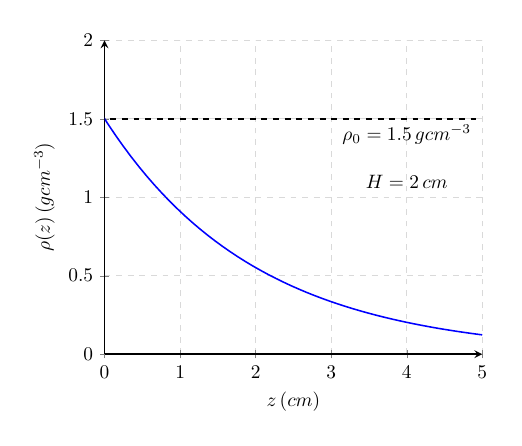
\begin{tikzpicture}[scale=0.7]
        \begin{axis}[
        ymin =0, ymax=2, 
        xmin=0, xmax=5, 
        xlabel = {$z \, (cm)$},
        ylabel = {$\rho(z) \, (gcm^{-3})$},
        grid = both,                % griglia
        grid style = {dashed, gray!30},
        axis lines = left,          % assi più puliti
        thick, % linee più spesse
    ]


    \addplot[color=blue, samples=100]{1.5*exp(-0.5*x)};
    \addplot[color=black, samples=25, dashed]{1.5}; 

     \node at (axis cs:4, 1.4) {$\rho_0 = 1.5\, gcm^{-3}$};
     \node at (axis cs:4, 1.1) {$ H = 2 \, cm$};

    \end{axis}
    \end{tikzpicture}

    \end{multicols}
}

\vspace{1cm}

\ex{}{
    Poniamoci ora a distanza $\vec{r}$ da una stella di massa $M$, e cosideriamo una struttura a simmetria assiale (e.g. un disco) in equilibrio idrostatico rispetto alla direzione $z$. In questo caso, l'eq. \ref{hydrostaatic_equilibrium} si scrive, lungo l'asse z: 
    \begin{equation}
    \frac{1}{\rho}\frac{dp}{dz} = -\frac{d\phi}{dz} = \frac{d}{dz}\left(\frac{GM}{|\vec{r}|} \right)
    \end{equation}

    Chiaramente data la simmetria assiale vorremo scrivere la derivata nel secondo termine dell'eq. in coordinate cilindriche $R, \theta, z$. Osserviamo che questa è data dalla forza di gravità lungo l'asse $z$, e sarà dunque data da
    \begin{equation}
        -\frac{GM}{r^2}\left(\frac{z}{r} \right) = -\frac{GMz}{(R^2 + z^2)^{3/2}} \simeq -\frac{GMz}{R^3} 
    \end{equation}
    Dove abbiamo fatto l'assunzione di $|z| << R$. Supponendo anche che il gas sia isotermo, 
    \begin{equation}
        p = c_s^2\rho
    \end{equation}
    Arriviamo dunque a scrivere 
    \begin{equation}
        c_s^2\frac{d\ln{\rho}}{dz} = -\underbrace{\frac{GM}{R^3}}_{=\Omega^2}z
    \end{equation}
    \begin{equation}
        \frac{d\ln{\rho}}{dz} = -\frac{z}{(c_s/\Omega)^2}
    \end{equation}
    Definendo prima $H = c_s/\Omega$, e poi la variabile adimensionale $y = z/H$, troviamo l'eq. differenziale 

    \begin{multicols}{2}

    \begin{equation}
        \frac{d\ln{\rho}}{dy} = -y \rightarrow \ln{\rho/\rho_0} = -y^2/2
    \end{equation}

    \vspace{-2cm}
    Così da ottenere, infine, 
    \begin{equation}
        \rho = \rho_0\exp\left(-\frac{z^2}{2H^2}\right)
    \end{equation}

    \columnbreak

    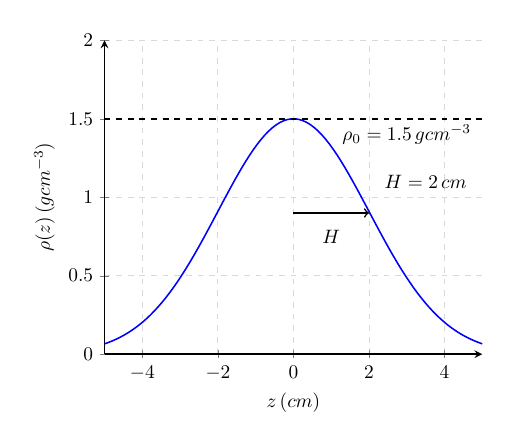
\begin{tikzpicture}[scale=0.7]
        \begin{axis}[
        ymin =0, ymax=2, 
        xmin=-5, xmax=5, 
        xlabel = {$z \, (cm)$},
        ylabel = {$\rho(z) \, (gcm^{-3})$},
        grid = both,                % griglia
        grid style = {dashed, gray!30},
        axis lines = left,          % assi più puliti
        thick, % linee più spesse
    ]


    \addplot[color=blue, samples=100]{1.5*exp(-0.125*x^2)};
    \addplot[color=black, samples=25, dashed]{1.5}; 

    \node at (axis cs:3, 1.4) {$\rho_0 = 1.5\, gcm^{-3}$};
    \node at (axis cs:3.5, 1.1) {$ H = 2 \, cm$};

    \draw[->, thick, black](axis cs: 0, 0.9) --(axis cs: 2, 0.9); 
    \node at (axis cs: 1, 0.75){$H$}; 

    \end{axis}
    \end{tikzpicture}
    \end{multicols}
}

\vspace{1cm}

\ex{}{
    Come ultimo esempio, prendiamo un calcolo effettuato per la prima volta in modo analitico da Spitzer, nel '42. Si tratta dello strato isotermo autogravitante. L'esempio ha chiare applicazioni in astrofisica, ad esempio per comprendere la base del funzionamento delle galassie. 

    Le equazioni sono
    \begin{equation}
        \frac{1}{\rho}\frac{dp}{dz} = -\frac{d\phi}{dz},  \, p = c_s^2 \rho, \, \nabla^2\phi = -4\pi G\rho 
    \end{equation}

    Usando il teorema di Gauss in modo simile ai conti tipici dell'elettromagnetismo, possiamo scrivere che la forza di gravità agente lungo $z$ sarà data da 
    \begin{equation}
        \vec{g}  = -4\pi G\sigma(z)\hat{z}, \, \sigma(z) = \int_0^z\rho(z^{'})dz{'}
    \end{equation}
    Sostituendo tutto nella eq. dell'equilibrio otteniamo 
    \begin{equation}
        \frac{c^2_s}{\rho}\frac{d\rho}{dz} = -4\pi G\int_0^z\rho(z^{'})dz{'}
    \end{equation}
    Effetuiamo una sostituzione nell'eq. per renderla un eq. di secondo grado, riconoscendo chiaramente che $\frac{d\sigma}{dz} = \rho$, 
    \begin{equation}
        c_s^2\frac{d^2\sigma}{dz^2} = -4\pi G \frac{d\sigma}{dz}\sigma
    \end{equation}
    Con condizioni al contorno $\sigma(0) = 0, \sigma^{'}(0) = \rho_0$. 
    Definisco in modo intelligente delle variabili adimensionali, 
    \[\begin{cases}
        \sigma = \sigma_0W \\
        z = z_0 y
    \end{cases}\]
    con $z_0 = \frac{c_s^2}{2\pi G\sigma_0}$, ed $\sigma_0 = \rho_0z_0$. 
    In questo modo, l'eq. differenziale diventa 
    \[\begin{cases}
        W^{''} = -2WW^{'} \\
        W(0) = 0 \\
        W^{'}(0) = 1
    \end{cases}\]

    Chiaramente la prima è equivalente a 
    \begin{equation}
        \frac{dW^{'}}{dy} = -\frac{d}{dy}(W^2) \rightarrow W^{'} - W^{'}(0) = W^2(0) - W^2
    \end{equation}

    Abbiamo dunque ridotto l'ordine dell'eq. e trovato 
    \begin{equation}
        W^{'} = 1 -W^2
    \end{equation}
    Osserviamo che se al membro di destra ci fosse stato $1 + W^2$, la soluzione sarebbe stata una $\tan^{-1}$. Poichè però c'è il segno meno, la soluzione è una tangente iperbolica: 

    \vspace{1cm}

    \begin{multicols}{2}
    
    \[\begin{cases}
        W(y) = \tanh{y} \\
        W^{'}(y) = \frac{1}{\cosh^2{y}}
    \end{cases}\]

    Ritornando alle variabili originarie, le soluzioni sono dunque date da 
    \begin{equation}
        \sigma(z) = \sigma_0 \tanh{z/z_0} \quad \rho(z) = \frac{\rho_0}{\cosh^2{z/z_0}}
    \end{equation}

    \columnbreak
    
    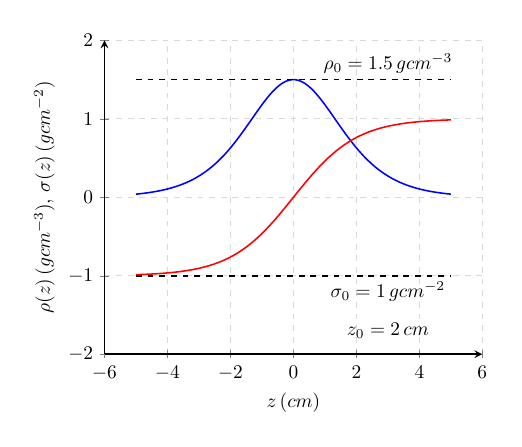
\begin{tikzpicture}[scale=0.7]
        \begin{axis}[
        ymin =-2, ymax=2, 
        xmin=-6, xmax=6, 
        xlabel = {$z \, (cm)$},
        ylabel = {$\rho(z) \, (gcm^{-3}), \, \sigma(z)\, (gcm^{-2})$},
        grid = both,                % griglia
        grid style = {dashed, gray!30},
        axis lines = left,          % assi più puliti
        thick, % linee più spesse
    ]


    \addplot[color=blue, samples=100]{1.5/(cosh(0.5*x))^2};
    \addplot[color=black, samples=25, dashed]{1.5}; 
    \addplot[color=black, samples=25, dashed]{-1}; 

    \node at (axis cs:3, 1.7) {$\rho_0 = 1.5\, gcm^{-3}$};
    \node at (axis cs:3, -1.7) {$ z_0 = 2 \, cm$};
    \node at (axis cs:3, -1.2) {$ \sigma_0 = 1 \, gcm^{-2}$};

    \addplot[color=red, samples=100]{tanh(0.5*x)};

    \end{axis}
    \end{tikzpicture}
    
    \end{multicols}
    
}

\section{Sfere politropiche}

Consideriamo un problema con immediate applicazioni all'astrofisica. Prendiamo un gas, in equilibrio con simmetria sferica, \emph{autogravitante}. Le equazioni allora sono date da 

\begin{equation}
    \label{politropic_equations}
    \frac{dp}{dr} = -\rho \frac{d\phi}{dr},  \quad \frac{1}{r^2}\frac{d}{dr}\left(r^2 \frac{d\phi}{dr} \right) = 4\pi G \rho
\end{equation}

Immediatamente da queste equazioni, possiamo concludere che il gas è barotropico (ovvero $p=p(\rho)$). Infatti, poichè chiaramente la densità $\rho$ è definita positiva, dalla prima equazione segue che o $p, \phi$ hanno la derivata sempre con lo stesso segno, oppure sempre con segno discorde. Questo è sufficiente a mostrare che la funzione $p=p(\phi)$ è ben definita e monotona. \\
D'altra parte, 
\begin{equation}
    \frac{dp}{dr} = \frac{dp}{d\phi}\frac{d\phi}{dr} = -\rho \frac{d\phi}{dr}
\end{equation}

e posso scrivere 
\begin{equation}
    \rho = -\frac{dp}{d\phi} \xrightarrow{p=p(\phi)} \rho = \rho(\phi)
\end{equation}

Invertendo $p=p(\phi)$ (che posso fare senza problemi perchè la funzione è monotona), ottengo $\phi = \phi(p)$, ed infine $\rho(\phi(p)) = \rho(p)$. Invertendo anche quest'ultima trovo che il gas, come promesso, è barotropico. \\

Aggiungiamo ora l'ipotesi che il gas sia politropico: questo vuol dire aggiungere alle eq. \ref{politropic_equations} l'eq. di stato 
\begin{equation}
    p = \mathcal{K}\rho^{1 + 1/n}
\end{equation}

Abbiamo allora un sistema di 3 equazioni in 3 incognite: inanzitutto, sostituiamo nell'eq. di Poisson l'eq. di equilibrio idrostatico, così da eliminare la dipendenza da $\phi$: 

\begin{equation}
    \frac{1}{r^2}\frac{d}{dr}\left(-\frac{r^2}{\rho} \frac{dp}{dr}\right) = 4\pi G\rho 
\end{equation}

Ora introduciamo delle comode variabili adimensionali. Scriveremo 
\begin{equation}
    r = \lambda\xi , \quad \rho = \rho_c \theta^n
\end{equation}
In questo modo l'eq. di stato politropica si scrive
\begin{equation}
    p = \mathcal{K}\rho_c^{1+1/n}\theta^{n+1}
\end{equation}

Per inserirla nell'equazione di poisson devo calcolare 
\begin{equation}
    \frac{dp}{dr} = \mathcal{K}\rho_c^{1 +1/n}(n+1)\theta^n\frac{d\theta}{dr} = \mathcal{K}\rho_c^{1/n}\rho(n+1)\frac{d\theta}{dr}
\end{equation}

La mia equazione è allora data da 
\begin{equation}
    \frac{1}{r^2}\frac{d}{dr}\left(r^2\mathcal{K}\rho_c^{1/n}(n+1)\frac{d\theta}{dr}\right) = -4\pi G \rho \xrightarrow{r =\lambda\xi} \frac{1}{\xi^2\lambda^2}\frac{d}{d\xi}\left( \xi^2\mathcal{K}\rho_c^{1/n}(n+1)\frac{d\theta}{dr}\right) = -4\pi G \rho
\end{equation}

Scegliendo dunque $\lambda^2 = \frac{\mathcal{K}\rho_c^{1/n}(n+1)}{4\pi G}$, otteniamo l'eq. di Lane-Emden di grado n \footnote{Se invece avessimo trattato il caso relativistico, l'eqauzione sarebbe diventata la famosa equazione di Tolman-Oppenheimer-Volkoff}: 
\begin{tcolorbox}[colback=myg!15, colframe=black, boxrule=1pt]
\begin{equation}
    \label{Lane_Emden_equations}
    \frac{1}{\xi^2}\frac{d}{d\xi}\left(\xi^2\frac{d\theta}{d\xi} \right) = -\theta^n , \quad \theta(0) = 1, \quad \theta^{'}(0) = 0
\end{equation}
\end{tcolorbox}

Le condizioni al controno sono giustificate dal fatto che la denisità al centro deve essere data da $\rho_c$, e che la forza al centro deve essere nulla. Infatti, notiamo che $\frac{dp}{dr} \propto \frac{d\theta}{dr}$, ma d'altra parte dall'equazione dell'equilibrio $\frac{dp}{dr} \propto \frac{d\phi}{dr}$. \\

Solo in alcuni casi è possibile risolvere l'eq. \ref{Lane_Emden_equations} analiticamete. Questi casi sono dati da: 

\begin{enumerate}
    \item $n=0$ \\
    In questo caso, la soluzione è data da 
    \begin{equation}
        \theta_0 = 1 - \frac{\xi^2}{6}
    \end{equation}
    Si tratta di una soluzione particolare, perchè si tratta di un corpo a densità costante ($\rho = \rho_c\theta^n = \rho_c$). In questo caso, si identifica la superficie della sfera come il punto dove la pressione si annulla, ovvero $\xi_0 = \sqrt{6} \simeq 2.45$
    \item $n=1$ \\
    La soluzione è data da 
    \begin{equation}
        \theta_1 = \frac{\sin{\xi}}{\xi}
    \end{equation}
    Poichè il problema ha senso finchè $\theta \geq 0$, la superficie è data da $\xi_1 = \pi$. Questo vuol dire che 
    \begin{equation}
        R = \lambda\xi = \sqrt{\frac{\pi \mathcal{K}}{2G}}
    \end{equation}
    ed osserviamo dunque che il raggio \emph{non} dipende dalla densità. 
    \item $n=5$ \\
    Si tratta del primo caso in cui la soluzione va a zero all'infinito. Questa è data da 
    \begin{equation}
        \theta_5 = \frac{1}{\sqrt{1 + \xi^2/3}}
    \end{equation}
\end{enumerate}

Il grafico riassume l'andamento delle soluzioni analitiche: 

\vspace{1cm}

\begin{center}
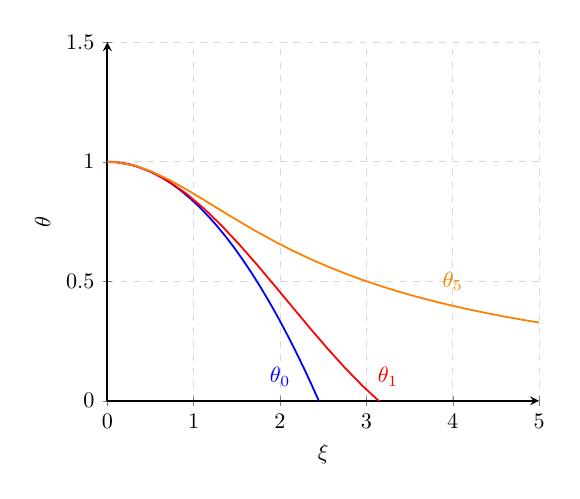
\begin{tikzpicture}[scale=0.8]
        \begin{axis}[
        ymin =0, ymax=1.5, 
        xmin=0, xmax=5, 
        xlabel = {$\xi$},
        ylabel = {$\theta$},
        grid = both,                % griglia
        grid style = {dashed, gray!30},
        axis lines = left,          % assi più puliti
        thick, % linee più spesse
    ]


    \addplot[color=blue, samples=100]{1-x^2/6};
    \addplot[color=red, samples=50]{sin(deg(x))/x};
    \addplot[color=orange, samples=50]{(1/(1+x^2/3))^(1/2)};


    \node at (axis cs:2, 0.1) [color=blue]{$\theta_0$};
    \node at (axis cs:3.25, 0.1) [color=red]{$\theta_1$};
    \node at (axis cs:4, 0.5) [color=orange]{$\theta_5$};

    %\draw[->, thick, black](axis cs: 0, 0.9) --(axis cs: 2, 0.9); 
    %\node at (axis cs: 1, 0.75){$H$}; 

    \end{axis}
    \end{tikzpicture}
    \end{center}

    \vspace{1cm}

    Veniamo ora alla determinazione della relazione \emph{massa-raggio} nelle sfere politropiche. 
    Chiaramente il raggio è dato da 
    \begin{equation}
        R = \xi_n\lambda = \xi_n\left[\frac{\mathcal{K}(n+1)}{4\pi G}\right]^{1/2}\rho_c^{\frac{1-n}{2n}}
    \end{equation}

    Mentre la massa è data da 
    \begin{equation}
        M = \int_0^R 4\pi r^2 \rho(r)dr = 4\pi \lambda^3 \rho_c \int_0^{\xi_n}d\xi\theta^n\xi^2
    \end{equation}

    Osserviamo che l'eq. \ref{Lane_Emden_equations} ci dice che $\theta^n\xi^2 = -\frac{d}{d\xi}\left(\xi^2\frac{d\theta}{d\xi} \right)$, così che potremo scrivere

    \begin{equation}
        M = 4\pi \lambda^3 \rho_c \int_0^{\xi_n} -\frac{d}{d\xi}\left(\xi^2\frac{d\theta}{d\xi} \right)d\xi = 4\pi \lambda^3\rho_c \left(-\xi^2 \theta^{'} \right)_{\xi = \xi_n}
    \end{equation}

    Definendo dunque la quantità (positiva) $g_n = \left(-\xi^2 \theta^{'} \right)_{\xi = \xi_n}$, otteniamo, esplicitando $\lambda$: 
    \begin{equation}
        M = 4\pi g_n\left[\frac{\mathcal{K}(n+1)}{4\pi G}\right]^{3/2}\rho_c^{\frac{3-3n}{2n}}
    \end{equation}

    Avendo $M=M(\rho_c), R = R(\rho_c)$ non ci resta che invertire le equazioni e con un po' di passaggi algebrici ottenere infine
    \begin{tcolorbox}[colback=myg!15, colframe=black, boxrule=1pt]
    \begin{equation}
        \label{mass_radius_politropic}
        M = 4\pi g_n \left[\frac{\mathcal{K}(n+1)}{4\pi G}\right]^{\frac{n}{n-1}}\left(\frac{R}{\xi_n} \right)^{\frac{3-n}{1-n}}
    \end{equation}
    \end{tcolorbox}

    Vediamo alcuni casi dove questa relazione ha delle applicazioni in astrofisica: 

    \begin{enumerate}
        \item $n = 3/2$ \\
        Si tratta del caso di un gas adiabatico. Questo tipicamente è un buon modello per le stelle completamente \emph{convettive}, della sequenza principale (con $M \lesssim 0.2 M_s$). Un altra situazione in cui questo si applica è un gas di elettroni degenere, in regime non relativistico. Per questo, si calcola
        \begin{equation}
            \mathcal{K} = \frac{1}{20}\left(\frac{3}{\pi} \right)^{2/3}\frac{h^2}{m_e}\left(\frac{1}{\mu_{mp}} \right)^{5/3}
        \end{equation}

        In effetti, questa è la composizione delle nane bianche con piccola massa.  Per queste, sperimentalmente si verifica la legge prevista dalla \ref{mass_radius_politropic}, ovvero $M \propto R^{-3}$. Questa legge invece non è rispettata dalle stelle nella sequenza principale però, dove sperimentalmente si osserca $M \propto R$. Come mai? il punto è che per questi sistemi la $\mathcal{K}$ non è un numero assegnato, ma dipende anche questa dalla densità. In effetti, se facciamo l'assunzione che la temperatura sia più o meno la stessa, possiamo scrivere 
        \begin{equation}
            T_c \propto \frac{p_c}{\rho_c} = \mathcal{K\rho_c}^{1/n} \xrightarrow{p_c \, stessa \, per \, tutte } \mathcal{K} \propto \rho_c^{1/2}
        \end{equation}

        Inserendo anche questo dato nelle eq. $M=M(\rho_c), R = R(\rho_c)$, scopriamo che $M \propto \rho_c^{-1/2}, R \propto \rho_c^{-1/2}$, il che giustifica le misure sperimentali. 
        \item $n=3$ \\
        Si tratta del caso dove il gas è dominato dalla pressione di radiazione. Di fatto offre un buon modello per le stelle radiative, dove l'energia viene trasportata grazie alla radiazione, come il sole, o le stelle con $M > 0.2 M_s$. L'eq. \ref{mass_radius_politropic} è piuttosto interessante perchè di dice $M = cost.$ ovvero tutte le stelle cosìfatte hanno la stessa massa. In particolare, rientrano in questa categoria un gas di elettroni degenere in regime relativistico: varrà allora 
        \begin{equation}
            \mathcal{K} = \frac{1}{8}\left(\frac{3}{\pi} \right)^{1/3}hc\left(\frac{1}{\mu_{mp}}\right)^{4/3}
        \end{equation}
        Da cui otteniamo la massa (detta di Chandrasekhar), 
        \begin{equation}
            M_{cs} = \sqrt{\frac{3}{\pi}}g_3\left(\frac{hc}{2G}\right)^{3/2}\left(\frac{1}{\mu_{mp}}\right)^2 
        \end{equation}
        
    \end{enumerate}

    \vspace{0.5cm}

    \begin{multicols}{2}
        Unendo le due informazioni sulle nane bianche di piccola massa e di grande massa, si ottiene il grafico raggio-massa delle nane bianche, rappresentato in figura. In particolare, osserviamo che non esiste una configurazione stabile per $M>M_{cs}$ (in figura posto =1). 

    \columnbreak

    \begin{tikzpicture}[scale=0.7]
        \begin{axis}[
        ymin =0, ymax=3, 
        xmin=0, xmax=2, 
        xlabel = {$M$},
        ylabel = {$R$},
        grid = both,                % griglia
        grid style = {dashed, gray!30},
        axis lines = left,          % assi più puliti
        thick, % linee più spesse
    ]


    \addplot[color=blue, dashed, samples=100]{x^(-1/3)};
    \addplot[color=blue, samples=100]{x^(-1/3)*(1-x^2)^(1/2)};


    \begin{pgfonlayer}{background}
            \fill[blue!10]  (axis cs:0,0)   rectangle (axis cs:1,3);
        \end{pgfonlayer}

    \node at (axis cs: 0.7, 2){regione};
    \node at (axis cs: 0.7, 1.8){stabile};

    \node at (axis cs: 1, 2.5)[color=red]{$M_{cs}$}; 
    \node at (axis cs: 1.5, 0.7)[color= red]{$x^{-1/3}$}; 
    \end{axis}
    \end{tikzpicture}

    
    \end{multicols}

    Studiamo ora il caso in cui il gas non è politropico ma è \emph{isotermo}. Questo vuol dire risolvere le equazioni
    \begin{equation}
        \frac{1}{\rho}\frac{dp}{dr} = -\frac{d\phi}{dr}, \, \frac{1}{r^2}\frac{d}{dr}\left(r^2 \frac{d\phi}{dr} \right) = 4\pi G \rho, \, p = c_s^2\rho
    \end{equation}
    Unendo le 3 con gli stessi passaggi del caso politropico, otteniamo l'eq. 
    \begin{equation}
        \frac{c_s^2}{r^2}\frac{d}{dr}\left(r^2\frac{d\ln{\rho}}{dr} \right) = -4\pi G\rho 
    \end{equation}

    Una banale soluzione di questa è data da una legge di potenza, ovvero $\rho = Ar^{-2}$. Se sostituiamo troviamo infatti 
    \begin{equation}
        -\frac{2c_s^2}{r^2}\frac{d}{dr}r = 4\pi G A \rightarrow A = \frac{c_s^2}{2\pi G}
    \end{equation}
    Dunque una soluzione è 
    \begin{equation}
        \rho(r) = \frac{c_s^2}{2\pi G r^2}
    \end{equation}

     Questa soluzione è detta \emph{sfera isoterma singolare}. Ha delle applicazioni in astrofisica perchè talvolta è presa come semplice modello per gli aloni di materia oscura. In ogni caso ha due problemi: è singolare nell'origine, e la massa $= \int 4\pi r^2 \rho(r)dr $ diverge linearmente. \\

     Per risolvere il primo problema, potremmo cercare delle soluzioni che abbiano densità \emph{finita} per $r=0$, ad esempio data da $\rho(0) = \rho_c$. Introduciamo allora una serie di parametri adimensionali: 
     \begin{equation}
         \lambda = \frac{c_s}{\sqrt{4\pi G \rho_c}} \rightarrow \xi = \frac{r}{\lambda}
     \end{equation}
     E scriveremo che la densità è data da 
     \begin{equation}
         \rho(r) = \rho_ce^{-\psi}, \, \psi(0) = 0 
     \end{equation}
     Sostitunendo, otteneniamo l'eq. differenziale 
     \begin{tcolorbox}[colback=myg!15, colframe=black, boxrule=1pt]
    \begin{equation}
        \label{isoterm_sfere}
        \frac{1}{\xi^2}\frac{d}{d\xi}\left(\xi^2\frac{d\psi}{d\xi} \right) = e^{-\psi}, \quad \psi(0)=0, \quad \psi'(0) = 0 
    \end{equation}
    \end{tcolorbox}

    Dove la condizione $\psi'(0) =0$ tiene conto che all'origine non deve esserci forza di gravità. La soluzione di quest'equazione è solamente numerica. Di fatto, il comportamento è il seguente: 
    \begin{enumerate}
        \item $r < \lambda$ \\
        La funzione rimane praticamente costante, seguendo una legge $\rho = \rho_c$. 
        \item $r > \lambda$ \\
        La funzione decresce, seguengo una legge di potenza, $\rho(r) \propto r^{-2}$. 
    \end{enumerate}

    Dal comportamento a grandi $r$, è chiaro che anche queste soluzioni hanno massa infinita. L'unico modo è troncare la soluzione ad un certo $\xi_0$. Chiaramente la diversa scelta di $\xi_0$ mi darà diverse soluzioni. Un'altro modo è troncare dato un paramentro di \emph{concentrazione}: 
    \begin{equation}
        g_0 = \frac{\rho_0}{\rho_c}
    \end{equation}
    Queste soluzioni sono dette sfere di Bonnor-Ebert. Poichè sono isoterme ed hanno densità finita al bordo, questo implica che, sempre al bordo, hanno una pressione finita. Vanno dunque sempre intese come immerse in un ambiente o mezzo che pareggi la loro pressione al bordo. \\

    Quanto vale la massa di una di queste sfere? Svolgiamo il conto: 
    \begin{equation}
        M = \int_0^{R_0}4\pi r^2 \rho(r)dr = \frac{4\pi \rho_c}{4\pi G \rho_c} \frac{c_s^3}{\sqrt{4\pi G\rho_c}}\int_0^{\xi_0}\xi^2 e^{-\psi}d\xi
    \end{equation}
    Ma l'eq. \ref{isoterm_sfere} ci dice che $\xi^2e^{-\psi} = \frac{d}{d\xi}\left(\xi^2 \psi'\right) $, così che otteniamo
    \begin{equation}
        M = \frac{c_s^3}{G\sqrt{4\pi G\rho_c}}\underbrace{(\xi_0^2 \psi'(\xi_0))}_{= f_0}
    \end{equation}
    Così che vale infine 
    \begin{tcolorbox}[colback=myg!15, colframe=black, boxrule=1pt]
    \begin{equation}
        M = \frac{c_s^3}{G\sqrt{4\pi G\rho_c}} f_0 = \frac{c_s^2}{G}R_0 \left(\frac{f_0}{\xi_0} \right)
    \end{equation}
    \end{tcolorbox}

    Vorremmo ora studiare le proprietà delle famiglie si sfere di Bonnor-Ebert aventi la stessa massa. In particolare ci chiediamo come variano $p_0, r_0$ in funzione l'uno dell'altro. 
    Per farlo, mi rendo conto che 
    \begin{equation}
        p_0 = c_s^2\rho_0 = c_s^2\rho_cg_0
    \end{equation}
    D'altra parte posso invertire la relazione per la massa:
    \begin{equation}
        4\pi G \rho_c = \frac{c_s^6}{(6M)^2}f_0 ^2
    \end{equation}
    Unendo le due, ottengo 
    \begin{equation}
        p_0 = \underbrace{\frac{c_s^8}{G^3M^2}}_{=p_s}\left(\frac{f_0^2g_0}{4\pi} \right) = p_s h(\xi_0)
    \end{equation}
    Ora voglio ottenere anche il raggio in funzione di $\xi_0$, che ottengo invertendo la relazione per la massa: 
    \begin{equation}
        R_0 = \frac{GM}{c_s^2}\left(\frac{\xi_0}{f_0} \right) = R_sl(\xi_0)
    \end{equation}

    Quando faccio un grafico della dipendenza paramentrica da $\xi_0$ di $P, R$, ottengo un grafico con due regioni distinte: 
    \begin{enumerate}
        \item $\xi < 6$ \\
        Per questa zona, il grafico sembra avere una legge di potenza del tipo $p \propto R^{-3}$. Questa non è altro che la legge di Boyle, $pV = cost. $. Chiaramente questa legge si perde per concentrazioni più grandi per effetto della gravità, ma per gas sufficientemente rarefatti è una buonissima approssimazione. 
        \item $\xi > 6$\\
        Curiosamente, il grafico fa un ricciolino. Si rivela che alcune regioni (con $p> p_{crit}$, o con $\rho < \rho_{crit}$) non vengono raggiunte. Di fatto, il ricciolino marca l'instabilità del fluido. Se il fluido si trova ad $\xi_0 > 6$, allora è un segno che questo collasserà. Questo è un primo esempio di collasso gravitazonale, ed è detto "catastrofe gravo-termica" oppure "instabilità di Bonnor-Ebert". Si calcola che la pressione critica è data da 
        \begin{equation}
            p_{crit} = (1.39)p_s = \frac{(1.39)c_s^8}{G^3M^2} 
        \end{equation}
    \end{enumerate}


\newpage

\chapter{Perturbazioni dell'equilibrio}

Come vedremo, molto spesso la perturbazione dell'equilibrio in un mezzo continuo porta alla generazione di un'onda che si propaga nel mezzo. Studiare le perturbazioni in questo caso vuol dire dunque studiare le proprietà di queste onde, a partire dalla fondamentale \emph{legge di dispersione}, che lega la pulsazione $\omega$, al vettore d'onda $\vec{k}$. In generale, per ottenerla si seguono i seguenti passaggi: 

\begin{enumerate}
    \item Definire lo stato di equilibrio
    \item Introdurre delle perturbazioni, $\rho = \rho_0 + \delta\rho, \quad \delta\rho/\rho <<1$. 
    \item Riscrivere le equazioni fluide in termini delle perturbazioni
    \item supporre che le perturbazioni si possano scrivere in termini di onde piane
    \item Ricavare la relazione di dispersione sostituendo le perturbazioni come onde piane nelle equazioni. 
\end{enumerate}

\section{Due approcci per le perturbazioni}

Ci chiediamo ora cosa voglia dire , in pratica, perturbare un fluido. Il modo più intuitivo di vederlo è considerare le traiettorie fluide: 

\begin{multicols}{2}

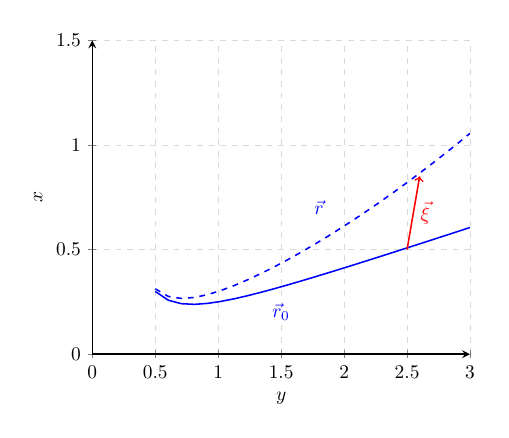
\begin{tikzpicture}[scale=0.7]
    \begin{axis}[
        ymin =0, ymax=1.5, 
        xmin=0, xmax=3, 
        xlabel = {$y$},
        ylabel = {$x$},
        grid = both,                % griglia
        grid style = {dashed, gray!30},
        axis lines = left,          % assi più puliti
        thick, % linee più spesse
    ]

    \addplot[color=blue, domain=0.5:3]{0.2*x + 0.05*x^(-2)};


    \addplot[color=blue, domain=0.5:3, dashed]{0.2*x + 0.05*x^(-2)+ 0.05*x^2};
    % Assi
    %\draw[->] (-0.2,0) -- (3,0) node[right] {$\rho/\rho_1$};
    %\draw[->] (0,-0.2) -- (0,2.2) node[above] {$P/P_1$};




    % Freccia che indica il senso del processo
    \draw[->,thick, red] (axis cs: 2.5,0.5) -- (axis cs: 2.6, 0.85) node[midway,right] {$\vec{\xi}$};

    % Etichette aggiuntive
    \node at (axis cs: 1.5,0.2) [color=blue]{$\vec{r}_0$};
    \node at (axis cs: 1.8,0.7) [color=blue]{$\vec{r}$};

    \end{axis}
    \end{tikzpicture}


    
\columnbreak

un elemento fluido seguirà una traiettoria $\vec{r}_0(\vec{x}_0, t)$ nel caso imperturbato, e una traiettoria $\vec{r}(\vec{x}, t)$ nel caso perturbato, come illustrato in figura. Chiaramente in generale al tempo $t$ varrà $\vec{r} \neq \vec{r}_0$, così che viene comodo definire il vettore di \emph{spostamento lagrangiano}: 

\vspace{-0.5cm}

\begin{align}
    \vec\xi(\vec{x}_0, t) &= \vec{r}(\vec{x}_0, t) - \vec{r}_0(\vec{x}_0, t)0 \\ &= \vec{\xi}(\vec{r}, t)
\end{align}

\end{multicols}



Consideriamo ora una qualsiasi proprietà del fluido $f= f(\vec{r}, t)$. Quanto vale la variazione di $f$ se perturbiamo il fluido? Anche qui, ci sono due modi per pensarlo. 
\begin{enumerate}
    \item Il modo euleriano\\
    Considero la quantità perturbata $f$ e la confronto con l'analoga imperturbata $f_0$ nello stesso punto. In questo modo non seguo però l'elemento fluido. 
    \item Il modo Lagrangiano\\
    Considero la variazione di $f$ su un elemento fluido, data dalla variazione intrinseca della proprietà + la variazione indotta dallo spostamento della traiettoria fluida. 
\end{enumerate}

Matematicamente questo si formalizza facilmente introducendo le quantità 
\begin{equation}
    \delta f = f(\vec{r}, t) - f_0(\vec{r}, t) \quad (perturbazione \ euleriana)
\end{equation}
\begin{equation}
    \Delta f = f(\vec{r}, t) - f_0(\vec{r}_0, t) \quad (perturbazione \ lagrangiana)
\end{equation}

Si noti che la prima commuta con derivate euleriane e gradienti, mentre la seconda commuta con derivate lagrangiane. Scrivendo $\vec{r} = \vec{r}_0 + \vec{\xi}$, fermandoci ai termini del primo ordine, possiamo chiaramente scrivere $f_0(\vec{r}_0, t ) \simeq f_0(\vec{r}, t ) - \vec{\xi}\cdot \vec{\nabla}f_0 \simeq f_0(\vec{r}, t ) - \vec{\xi}\cdot \vec{\nabla}f$, così da ricavare l'importante relazione fra le due quantità:

 \begin{tcolorbox}[colback=myg!15, colframe=black, boxrule=1pt]
\begin{equation}
    \Delta f = \delta f + \vec{\xi}\cdot\vec{\nabla}f
\end{equation}
\end{tcolorbox}

Le due formulazioni sono dunque equivalenti qualora $f$ fosse uniforme. \\
Un'importante quantità di cui potremmpo ricavare la perturbazione lagrangiana e la velocità fluida: 
\begin{equation}
    \Delta \vec{u} = \vec{u}(\vec{r}, t) + \vec{u}_0(\vec{r}_0, t)
\end{equation}

Ricordandomi ora che la velocità è la derivata rispetto al tempo della posizione, e della definizione del vettore spostamento lagrangiano, scriveremo semplicemente 
\begin{equation}
    \Delta \vec{u} = \frac{D\xi}{Dt} = \frac{\partial \xi}{\partial t} + (\vec{u}\cdot \vec{\nabla})\vec{\xi}
\end{equation}

In particolare, se l'equilibrio inziale è idrostatico, allora la derivata euleriana e lagrangiana si equivalgono. 

Vediamo una veloce applicazione di questo: supponiamo di avere un equilibrio tale per cui $\vec{u}_0 = 0$, $\partial_t \rho_0 = 0$. Scriviamo in questo caso l'eq. di continuità per le perturbazioni: 

\begin{align}
    \frac{\partial}{\partial t}(\delta \rho) + \vec{\nabla}\cdot (\rho_0\vec{u}) = \frac{\partial}{\partial t}(\delta \rho) + \rho_0\vec{\nabla}\cdot\vec{u} + \vec{u}\cdot \vec{\nabla}\rho_0 
\end{align}

Ora possiamo integrare l'espressione rispetto al tempo, per ottenere
\begin{align}
    \delta \rho + \rho_0 \vec{\nabla}\cdot \xi + \vec{\xi}\cdot \vec{\nabla}\rho_0 = \Delta\rho + \rho_0 \vec{\nabla}\cdot \vec{\xi}
\end{align}

Dove abbiamo usato l'ipotesi che $\rho_0$ non dipendesse dal tempo e la relazione fra la perturbazione della velocità e il vettore di spostamento lagrangiano. Abbiamo dunque ottenuto l'interessante relazione
\begin{align}
    \frac{\Delta \rho}{\rho_0} = - \vec{\nabla}\cdot \vec{\xi}
\end{align}
\section{Un primo esempio, le onde sonore}

Consideriamo come configurazione di equilibrio un fluido uniforme e stazionario. Questo ha $\rho = cost. , \, p= cost.\,, \vec{u}_0=0$. Soddisfa le equazioni di continuità e di eulero nel caso di forze esterne assenti. Introduciamo dunque le perturbazioni: 
\[\begin{cases}
    \rho = \rho_0 + \delta\rho \\ p = p_0 + \delta p \\ \vec{u} = \delta \vec{u}
\end{cases}\]

Per prima cosa calcoliamo l'eq. di continuità: 

\begin{equation}
    \frac{\partial \rho_0}{\partial t} + \frac{\partial \delta \rho}{\partial t} + \vec{\nabla} \cdot ((\rho_0 + \delta\rho)\vec{u}) = \frac{\partial \delta \rho}{\partial t} + \rho_0\vec{\nabla} \cdot\vec{u} 
\end{equation}

Poi l'equazione di eulero: 
\begin{equation}
    \frac{\partial \vec{u}}{\partial t} = -\frac{1}{\rho_0 + \delta\rho}(\vec{\nabla}p_0 + \vec{\nabla}\delta p) = -\frac{1}{\rho_0}(1 - \delta\rho/\rho_0)/(\underbrace{\vec{\nabla}p_0}_{=0} + \vec{\nabla}\delta p) = -\frac{1}{\rho_0}\vec{\nabla}\delta p
\end{equation}

Come equazione di stato, assumiamo semplicemente che il fluido sia barotropico, così che valga $p = p(\rho)$. L'eq di eulero è allora data da 
\begin{equation}
    \frac{\partial \vec{u}}{\partial t} = -\frac{1}{\rho_0}\left(\frac{dp}{d\rho} \right)\vec{\nabla}\delta \rho
\end{equation}
Ne prendo allora la divergenza, al fine di combinarla con l'eq. di continuità
\begin{equation}
    \frac{\partial (\vec{\nabla}\cdot\vec{u})}{\partial t} = -\frac{1}{\rho_0}\left(\frac{dp}{d\rho} \right)\nabla^2\delta \rho
\end{equation}
e sostituendo $\vec{\nabla}\cdot \vec{u} = -\frac{1}{\rho_0}\frac{\partial \delta \rho}{\partial t}$, si ottiene 

\begin{tcolorbox}[colback=myg!15, colframe=black, boxrule=1pt]
\begin{equation}
    \frac{\partial ^2 \delta\rho}{\partial \delta\rho^2} - \left(\frac{dp}{d\rho} \right)\nabla^2\delta \rho = 0 
\end{equation}
\end{tcolorbox}

Che è l'equazione delle onde di D'Alambert! da qui la convenzione di chiamare spesso 
\begin{equation}
    \frac{dp}{d\rho} = c_s^2
\end{equation}
poichè per un fluido barotropico, questa è proprio la velocità del suono. Una soluzione dell'equazione è un onda piana, ovvero $\delta\rho \propto e^{i(\omega t - \vec{k}\cdot \vec{r})}$. Sostituendo questa nell'eq. delle onde, troviamo 
\begin{align}
    -\omega^2\delta\rho + k^2c_s^2\delta\rho = 0 \rightarrow \omega^2 = c_s^2k^2
\end{align}

che è la relazione di dispersione che stavamo cercando! Sostituendo ancora nell'equazione di continuità scopriamo che 
\begin{equation}
    \frac{\delta\rho}{\rho_0} = \frac{\vec{k}\cdot \vec{u}}{\omega}
\end{equation}
e facendo lo stesso per eulero
\begin{equation}
    \vec{u} = \frac{c_s^2 \vec{k}}{\omega}\frac{\delta \rho}{\rho_0}
\end{equation}
Questa ci dice che $\vec{u} \parallel \vec{k}$, ovvero l'onda è un onda longitudinale! D'altra parte, sapendo questo possiamo passare ai moduli nell'equazione ricavata dalla continuità, 
\begin{equation}
    \frac{\delta \rho}{\rho_0} = \frac{ku}{\omega} = \frac{u}{c_s}
\end{equation}

Che ci dice che l'approssimazione lineare è buona finche $u << c_s$. \\

Veniamo ora alla discussione su che tipo di equazione di stato scegliere. Abbiamo supposto fino ad ora una legge barotropica, ma come scelgo se un fenomeno è adiabatico oppure isotermo? Di fatto, per poterlo considerare isotermo, le oscillazioni devono essere a scale di tempo minori del tempo $t_{cool}$ in cui il sistema raggiunge l'equilibrio. I regimi dunque dove $\omega t_{cool} >>1$ sono dunque adiabatici, mentre $\omega t_{cool} << 1$ possono essere considerati isotermi. Si noti che questo è completamente indipendete dal sistema all'equilibrio, dunque vi sono situazioni dove il fluido all'equilibrio è isotermo, ma le oscillazioni sono talmente veloci che il corretto regime da considerare per queste è quello adiabatico. 

\section{Perturbazioni in mezzi stratificati}

Cosa succede quando consideriamo mezzi non più omogenei? Questa è una domanda lecita perchè in questi casi le perturbazioni lagrangiane ed euleriane sono diverse tra di loro. L'esempio più semplice da fare è l'atmosfera: prendiamo come sistema all'equilibrio un fluido isotermo soggetto ad una forza costante lungo la direzione $z$. Abbiamo già visto che la soluzione per le eq. dell'equilibrio di un dato sistema sono date da 

\begin{equation}
    \rho_0 = \hat{\rho}e^{-z/H}, \quad H = c_s^2/g, \quad c_s^2 = \frac{p_0}{\rho_0} = \frac{\mathcal{K}T}{\mu_{mp}}
\end{equation}

Le equazioni del moto per questo sistema, interessandoci solo alla componente $z$ e supponendo che valga $\vec{u} = (0, 0, u) = u\hat{z}$ sono date da 

\begin{equation}
    \frac{\partial \rho}{\partial t} + \frac{\partial}{\partial z}(\rho u) = 0 
\end{equation}
e da 
\begin{equation}
    \frac{\partial u}{\partial t} + u\frac{\partial u}{\partial z} = -\frac{1}{\rho}\frac{\partial p}{\partial z} - g
\end{equation}

Scrivendo $\rho = \rho_0 + \rho_1$ e mantenendo le quantità al primo ordine scriveremo

\begin{equation}
    \frac{\partial \rho_1}{\partial t} + \frac{\partial \rho_0}{\partial z}u + \frac{\partial u}{\partial z}\rho_0 = \frac{\partial \rho_1}{\partial t} -\frac{\rho_0 u}{H} + \rho_o \frac{\partial u}{\partial z} = 0
\end{equation}

\begin{equation}
    \frac{\partial u_1}{\partial t} = -\frac{1}{\rho_0 + \rho_1}\left(\partial_z p_0 + \partial_z p_1\right) - g \simeq -\frac{1}{\rho_0}\left(1 - \frac{\rho_1}{\rho_0} \right)(\partial_z p_0 + \partial_zp_1) - g = -\frac{1}{\rho_0}\left(\partial_z p_1 + \frac{c_s^2}{H}\rho_1\right)
\end{equation}

Volendo unire le due, deriviamo rispetto al tempo la secodnda e rispetto a $z$ la seconda: 

\begin{equation}
    \partial_t^2 u_1 = -\frac{1}{\rho_0}(\partial_t\partial_z p_1 + c_s^2 \partial_t\frac{\rho_1}{H})
\end{equation}
\begin{equation}
    \partial_z\partial_t \rho_1 - \rho_0 \frac{\partial_z u}{H} + u \frac{\rho_0}{H^2} + \rho_0 \partial^2_z u - \partial_z u \frac{\rho_0}{H} = 0
\end{equation}

Le equazioni sono due ma abbiamo ancora 3 incognite: è tempo di inserire l'eq. di stato, che supponiamo essere isoterma o adiabatica. Nel primo caso, si prende $\gamma = 1$. L'eq. di eulero diventa

\begin{equation}
    \partial^2_t u_1 = -\frac{1}{\rho_0}\left(\gamma c_s^2 \partial_z\partial_t \rho_1 + c_s^2 \partial_t \frac{\rho_1}{H}\right)
\end{equation}

Ora sostituisco il termine $\partial_z\partial_t\rho_1$ con l'eq. di continuità derivata e il termine $\partial_t\rho_1$ con quella non derivata: dopo un po' di algebra, si arriva a scrivere

\begin{equation}
    \partial^2_t u_1 = \gamma c_s^2 \partial^2_z u_1 + (2\gamma -1)\frac{\partial_z u_1}{H} - (\gamma -1)c_s^2 \frac{u_1}{H^2}
\end{equation}

Questa equazione è \emph{sbagliata}. Questo perchè l'approccio euleriano è problematico quando uso l'eq. di stato. Non c'è modo di assicurarmi infatti che io non mischi gli elementi fluidi quando uso le leggi della termodinamica. Vedremo usando l'approccio lagrangiano che solo il caso isotermo (i.e. $\gamma = 1$) è corretto, tutti gli altri sono sbagliati. \\

Vediamo il risultato che otteniamo usando l'aproccio lagrangiano. In particolare, scriviamo le nostre quantità perturbate: 

\begin{align}
    \Delta \rho &= \delta\rho + \xi\partial_z\rho = \delta\rho - \xi \frac{\rho_0}{H} \\
    \Delta p &= \delta p - \xi \frac{p_0}{H} \\
    \Delta u &= \frac{\partial \xi}{\partial t}
\end{align}

Consideriamo le equazioni perturbate al primo ordine, ad esempio l'eq. di continuità: 

\begin{equation}
    \partial_t(\delta \rho) + \rho_o (\partial_z u) - u\frac{\rho_0}{H} = 0 
\end{equation}

e la scriviamo in termini della variazione lagrangiana: 

\begin{align}
    &\partial_t(\Delta \rho) + \underbrace{\partial_t(\xi)}_{=u} \rho_0/H + \rho_0(\partial_z u) - u\frac{\rho_0}{H} = 0 \\
    &\partial_t(\Delta \rho) + \rho_0(\partial_zu) = 0 
\end{align}

Ora ci occupiamo di eulero: 

\begin{align}
    \partial_t u &= -\frac{1}{\rho_0}\left(1 - \frac{\delta\rho}{\rho_0} \right)\left(\partial_z p_0 + \partial_z \delta p \right) - g \\
    &= -\frac{1}{\rho_0}\left(\partial_z \delta p - \frac{\delta \rho}{\rho_0}\partial_zp_0 \right) = -\frac{1}{\rho_0}\left(\partial_z \delta p - \frac{\delta\rho}{\rho_0}\frac{p_0}{H} \right) \\ &= -\frac{1}{\rho_0}\partial_z\left(\Delta p + \xi \frac{p_0}{H}\right) + \frac{1}{\rho_0}\left(\frac{p_0}{\rho_0 H} (\Delta \rho + \xi \frac{\rho_0}{H})\right) \\ & = -\frac{1}{\rho_0}\partial_z\left(\Delta p + \xi \frac{p_0}{H}\right) + \frac{c_s^2}{\rho_0}\left(\frac{1}{H} (\Delta \rho + \xi \frac{\rho_0}{H})\right) \\
    &= -\frac{1}{\rho_0}\partial_z\left(\Delta p + \xi \frac{p_0}{H}\right) + \frac{c_s^2}{H}\left(\frac{\Delta \rho}{\rho_0} + \xi \frac{\rho_0}{H}\right)
\end{align}

La maggior parte delle cose si cancellano e troviamo infine 
\begin{equation}
    \partial_tu = -\frac{1}{\rho_0}\partial_z(\Delta p) = -\frac{\gamma c_s^2}{\rho_0}\partial_z(\Delta \rho)
\end{equation}

Ora derivo rispetto al tempo

\begin{equation}
    \partial_t^2 u = -\frac{\gamma c_s^2}{\rho_0}\partial_z(\partial_t(\Delta\rho_))
\end{equation}

Sostituisco $\partial_t(\Delta \rho)$ usando l'eq. di continuità: 
\begin{equation}
    \partial_t^2 u = +\frac{\gamma c_s^2}{\rho_0}\partial_z(\rho_0 \partial_zu) = \gamma c_s^2 \partial_z^2 u + \gamma c_s^2 (\partial_zu)\frac{\partial_z\rho_0}{\rho_0}
\end{equation}

Otteniamo così infine 

\begin{tcolorbox}[colback=myg!15, colframe=black, boxrule=1pt]
\begin{equation}
    \partial_t^2u = \gamma c_s^2 \left[\partial_z^2u - \frac{\partial_z u}{H}\right]
\end{equation}
\end{tcolorbox}

Che è l'equazione che stavamo cercando. Coincide con la formula elueriana per $\gamma=1$. \\

Per trovare la relazione di dispersione, dobbiamo ipotizzare che un onda piana sia soluzione di questa equazione. Come faccio però visto che non conosciamo le sue soluzioni? Osserviamo che però in questo caso la scelta di onde piane è sempre lecita, perchè la simmetria rispetto al tempo ci permette sempre di prendere soluzioni del tipo $u(z, t) = e^{i(\psi(z)- \omega t)}$, e d'altra parte sviluppando $\psi$ in serie di Taylor, 

\begin{equation}
    \psi(z) \simeq \psi_0 + \frac{d\psi}{dz}\biggr|_{z=0}z
\end{equation}

Ritroviamo un'onda piana con $ k = \frac{d\psi}{dz}\biggr|_{z=0}$, ed una fase irrilevante. Sostituendo nell'eq. troviamo allora la relazione di dispersione: 

\begin{equation}
    \omega^2 = c_A^2 k^2\left(1 + \frac{i}{kH} \right)
\end{equation}

Chiaramente non essendo lineare, sarà una relazione \emph{dispersiva}. Risolvendo per $k$, si trova in particolare

\begin{equation}
    k = -\frac{i}{2H} \pm \sqrt{\left(\frac{\omega}{c_a}\right)^2 - \left(\frac{1}{2H}\right)^2}
\end{equation}

Esaminiamo cosa questo implica in due limiti: 

\begin{enumerate}
    \item limite di alte frequenze $\omega / c_a > 1/2H$: \\ $k$ è un numero complesso avente sia parte reale che immaginaria. Nel dettaglio varrà 
    \begin{align}
        &Re(k)^2 = \left(\frac{\omega}{c_a}\right)^2 - \left(\frac{1}{2H}\right)^2 \\ &Im(k) = -\frac{1}{2H}
    \end{align}
    Questo vuol dire che l'andamento sarà oscillante modulato da una crescita esponenziale $u \propto e^{z/2H}$(che porta poi la perturbazione a diventare supersonica). Questo fenomeno è controintuitivo perchè nell'esperienza comune, effetti dissipativi non permettono ad un suono di propagarsi fino alla fine dell'atmosfera. Si può ciononostante comprendere intuitivamente come una conseguenza per la conservazione dell'energia, che sarà data da 
    \begin{equation}
        E = \frac{1}{2}\rho u^2 = cost. 
    \end{equation}
    D'altra parte, poichè vale $\rho \propto e^{-z/H}$, allora varrà $u \propto e^{z/2H}$, che è proprio quello che abbiamo trovato. Uno può anche chiedersi quale sia la velocità di gruppo e di fase, che si trovano essere (con le solite formule)
    \begin{align}
        & v_{ph} = c_A\left(1 - \left(\frac{c_a}{2\omega H}\right)^2\right)^{-1/2} \\
        & v_{g} = c_A\left(1 - \left(\frac{c_a}{2\omega H}\right)^2\right)^{1/2}
    \end{align}
    \item limite di basse frequenze $\omega / c_a < 1/2H$ : \\
    In questo caso c'è poco da dire, perchè $k$ diventa un numero puramente immaginario. Non vi sono osclizzazioni, solo onde stazionare. Di fatto, possiamo pensare che la dispersione agisca come una riflessione efficace. 
\end{enumerate}

\section{Onde d'urto}

Quando abbiamo ricavato l'eq. delle onde come equazione per le piccole perturbazioni dell'equilibrio statico, abbiamo anche osservato che 
\begin{equation}
    \frac{\delta \rho}{\rho_0} = \frac{u}{c_s}
\end{equation}

Che ci dice che l'approssimazione lineare delle perturbazioni è valida solo per perturbazioni \emph{subsoniche}. Ora vorremmo indagare cosa succede se vale $u> c_s$. Il risultato di queste forti perturbazioni sono le \emph{onde d'urto}, oppure shock-wave. \\

Immaginiamo il seguente esempio: un proiettile che attraversa un fluido, con velocità $v >> c_s$: il proiettile mano a mano che viaggia modifica le condizioni al contorno del fluido, nel senso che impone al fluido di disporsi lungo i suoi bordi. D'altra parte, il fluido ha bisogno di tempo per riassestarsi, e per diversi istanti si crea una discontinuità nel fluido. Ciò che questo ci dice che non possiamo utilizzare il calcolo differenziale per trattare le onde d'urto! \\

Naturalmente, globalmente leggi come la conservazione della massa continuano a valere, così che potremo comunque impostare delle condizioni globali passando da equazioni in forma differenziale alla loro versione integrale. Questo tipo di equazioni per studiare le onde d'urto sono note come \emph{relazioni di Rankine-Hugoniot}. Convertiamo dunque in questo modo le equazioni fluide: 

\begin{enumerate}
    \item Equazione di continuità \\
    Per comodità, considereremo sempre uno schok in una dimensione. Questa può sembrare un'ipotesi molto vincolante, soprattutto se pensiamo ad onde d'urto con profili complessi. D'altra parte, se guardiamo abbastanza vicino qualsiasi profilo può essere visto come un piano, così che questa idealizzazione ci permette in realtà di capire tutta la fisica del fenomeno. \\

    Immagiamo dunque lo schock su un piano, che divide due regioni di spazio. A causa della discontinuità che lo schock implica nelle due regioni avrò, in generale, $u_2 \neq u_1, \, p_1 \neq p_2, \, \rho_1 \neq \rho_2$. Ora prendo un rettangolo in modo tale che le facce siano parallele agli assi ed integro nel suo volume $V$ l'eq. di continuità: 

    \begin{equation}
        \frac{\partial \rho}{\partial t} + \frac{\partial}{\partial x}(\rho u) = 0 \rightarrow \frac{\partial}{\partial t} \int_V \rho d^3x + \int_V\frac{\partial u}{\partial x}d^3x = 0  
    \end{equation}

    Ora osservo che la discontinuità è solo lungo la direzione $x$, così che posso fare tendere a $0$ i lati del rettangolo paralleli ad $x$: in questo modo la prima parte si semplifica e la seconda si riduce a 
    \begin{tcolorbox}[colback=myg!15, colframe=black, boxrule=1pt]
    \begin{equation}
        (\rho u)|^2_1 = 0 \rightarrow \rho_1u_1 = \rho_2u_2
    \end{equation}
    \end{tcolorbox}
    \item Equazione di Eulero \\
    Imparato il trucco del rettangolo con i lati che vanno a $0$, il procedimento è lo stesso per tutte le equazioni, basta sceglierle nella forma di leggi di conservazione. Prendiamo dunque eulero 
    \begin{equation}
        \frac{\partial }{\partial t}(\rho u) = - \frac{\partial}{\partial x}(\rho u^2 + p) - \rho \frac{\partial \phi}{\partial x}
    \end{equation}
    Questa integrata ci dice che
    \begin{equation}
        \int \frac{\partial}{\partial x}(\rho u^2 +p)dx =0 
    \end{equation}
    che semplicemente implica 
    \begin{tcolorbox}[colback=myg!15, colframe=black, boxrule=1pt]
    \begin{equation}
        \rho_1u_1^2 + p_1  =\rho_2 u_2^2 + p_2
    \end{equation}
    \end{tcolorbox}

    In realtà, abbiamo solo considerato l'eq. di Eulero diretta lungo l'asse $x$, a l'eq. di eulero è vettoriale, quindi ci può dare informazioni su le componenti $y, z$ di $u_1, u_2$. In particolare, si ha 
    \begin{equation}
        \partial_t(\rho u_i) = -\partial_j(\rho u_i u_j + p\delta_{ij})
    \end{equation}
    Con gli stessi conti trovati prima, si ottiene, lungo un qualunque versore $\hat{n}$: 
    \begin{equation}
        n_i(\rho u_iu_j +p\delta_{ij})|^2_1 =0
    \end{equation}

    Se prendiamo $i=j$ allora troviamo l'espressione precedente, se invece prendiamo $i\neq j$ allora abbiamo due possibilità:

    \begin{align}
        & \rho u_xu_y |^2_1 = 0 \\
        & \rho u_x u_z |^2_1 = 0 
    \end{align}

    Ricordando però che $\rho u_x$ si conserva per la prima condizione di Rankine-Hugoniot, otteniamo semplicemente che 
    \begin{align}
        &u_{y, 1} = u_{y, 2} \\ &u_{z, 1} = u_{z, 2}
    \end{align}

    \item Equazione dell'energia \\
    Scriviamo, per un fluido non gravitante, 
    \begin{equation}
        E = \rho \epsilon + \frac{1}{2}\rho u^2 + \rho \phi_{ext}
    \end{equation}
    Così che l'eq. dell'energia è data da 
    \begin{equation}
        \frac{\partial E}{\partial t} = -\partial_j((E+p)u_j) + \rho\dot{Q}
    \end{equation}
    Ora, chiaramente la condizione di Rankine-Hugoniot per l'energia dipende fortemente dal tipo di processo di riscaldamento o raffreddamento che stiamo considerando. In particolare, vi sono due situazioni molto importanti: il caso \emph{adiabatico} ed il caso \emph{isotermo}. Quale ci interessa in base alla situazione? In realtà non esistono urti adiabatici o isotermi: se guardo a scale temporali molto piccole, allora un'onda d'urto è sempre adiabatica, se aspetto un tempo sufficiente l'onda d'urto è sempre isoterma. In effetti, il grafico della temperatura di un fluido dopo l'onda d'urto è piuttosto universale: \\

    \begin{center}
        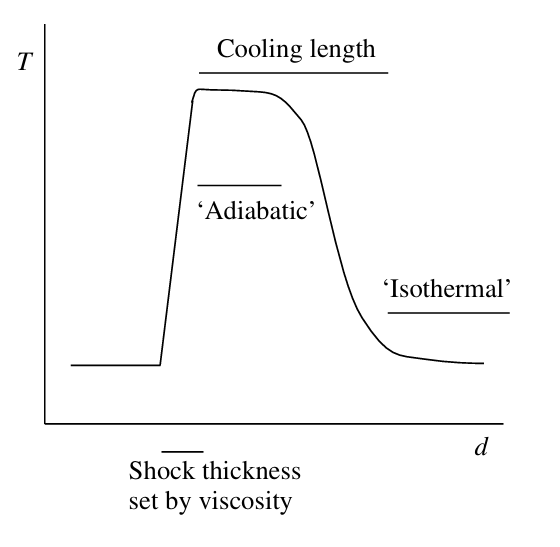
\includegraphics[scale = 0.5]{shock-temperature.png}
    \end{center}

    Vediamo dunque cosa succede per il caso adiabatico. Prenderemo $\dot{Q}=0$, così che integrando l'eq. dell'energia troveremo 
    \begin{equation}
        (E+p)u|^2_1 = 0 \rightarrow [(\epsilon + u^2/2 + p/\rho )\rho u]|^2_1 =0
    \end{equation}

    Ricordandomi che il prodotto $\rho u$ si conserva per la prima condizione, scriveremo 
    \begin{tcolorbox}[colback=myg!15, colframe=black, boxrule=1pt]
    \begin{equation}
        \epsilon_1 + \frac{u_1^2}{2} + \frac{p_1}{\rho_1} = \epsilon_2 + \frac{u_2^2}{2} + \frac{p_2}{\rho_2}
    \end{equation}
    \end{tcolorbox}
    In effetti, questa equazione ha molte formulazioni equivalenti. Ad esempio, se ho un gas perfetto vale 
    \begin{equation}
        \epsilon = \frac{1}{\gamma -1}\frac{p}{\rho}
    \end{equation}
    Così che la condizione diventa, ricordandomi anche che $c_s^2 = \gamma p/\rho$, 
    \begin{equation}
        \frac{1}{2}u_1^2 + \frac{c_{s, 1}^2}{\gamma-1} = \frac{1}{2}u_2^2 + \frac{c_{s, 2}^2}{\gamma-1} 
    \end{equation}

    Questa si scrive anche, dopo alcuni passaggi algebrici, 
    \begin{equation}
        \frac{\rho_2}{\rho_1} = \frac{u_1}{u_2} = \frac{(\gamma +1)p_2 + (\gamma -1)p_1}{(\gamma +1)p_1 + (\gamma -1)p_2} 
    \end{equation}

    Il che mostra che se ho uno shok forte, ovvero ho $p_2 >> p_1$, allora avrò che 
    \begin{equation}
        \frac{u_1}{u_2} = \frac{\gamma +1}{\gamma -1}
    \end{equation}
    Ovvero per un gas monoatomico $u_1 = 4u_2$, $\rho_2 = 4\rho_1$. Consideriamo adesso l'entropia, che sappiamo dipendere da $p\rho^{-\gamma}$. Ora in uno scock forte, $p_2 >> p_1$, ma le densità rimangono dello stesso ordine. Segue che l'entropia aumenta di molto, o in altre parole le onde d'urto sono processi \emph{irreversibili}. \\

    Un'altro modo di scrivere l'eq. per i gas perfetti è in termini del numero di Mach (i.e. il rapporto fra la velocità e la velocità del suono): 
    \begin{equation}
        m_2^2  = \frac{2 + (\gamma -1)m_1^2}{2\gamma m_1^2 - (\gamma -1)}
    \end{equation}
    In particolare, se lo shock è forte varrà 
    \begin{equation}
        m_2^2 \simeq \frac{\gamma -1}{2\gamma} < 1
    \end{equation}
    Questo ci dice che il fluido dopo lo schock è sempre subsonico. Questo non è una conseguenza del cambiamento della velocità, perchè questo è dell'ordine dell'unità, ma è invece conseguenza dell'aumento della velocità del suono. \\

    Il caso isotermo è invece più banale. Di fatto l'eq. dell'energia ci dice $T_1 = T_2$. Unsando l'eq. di stato per i gas perfetti, possiamo scrivere 
    \begin{equation}
        \rho_1(u_1^2 + c_s^2) = \rho_2(u_2^2 + c_s^2)
    \end{equation}
    Che con un po' di manipolazioni mi dice 
    \begin{equation}
        c_s^2 = u_1u_2
    \end{equation}
    oppure 
    \begin{equation}
        m_1m_2 = 1
    \end{equation}

    Questo ad esempio mi dice che, se lo shock è forte ($m_1 >>1$)
    \begin{equation}
        \frac{\rho_2}{\rho_1} = \frac{m_1}{m_2} = m_1^2 >>1
    \end{equation}
    Il che significa che la densità aumenta molto, come risultato del rallentamento del fluido. 
\end{enumerate}

\newpage
\chapter{Instabilità}

Rivolgiamo ora la nostra attenzione a perturbazioni instabili. La prima domanda è naturale? Come ci si rende conto in generale se una perturbazione è instabile? \\

In generale, per prendere la relazione di dispersione, noi supponiamo che la perturbazione si propaghi come un onda piana, ovvero come 
\begin{equation}
    \exp[i(\vec{k}\cdot \vec{r} - \omega t)]
\end{equation}

Ora, se per caso valesse $\text{Im}(\omega) > 0$, allora avremmo che la perturbazione evolve col tempo crescendo esponenzialmente, allontanando il sistema dalla configurazione stabile. Vediamo qualche tipico esempio di instabilità. 

\section{Instabilità gravitazionale}

L'instabilità gravitazionale è un processo fondamentale in astrofisica. Questo è alla base della formazione di tutte le strutture, dagli aloni di materia oscura alle stelle. Vediamo due tipi di instabilità in mezzi autogravitanti, il caso di un mezzo omogeneo, ed il caso di uno strato isotermo rotante. 

\subsection{Teoria di Jeans}

Consideriamo un mezzo barotropico, autogravitante, con $\rho_0 = cost.$, $p_0 = cost.$, $\vec{u}=0$. Il set di equazioni che deve soddisfare è dato da 
\begin{align}
    &\frac{\partial \rho}{\partial t} + \vec{\nabla}\cdot \rho \vec{u} = 0 \\
    & \frac{\partial \vec{u}}{\partial t} + (\vec{u}\cdot \vec{\nabla})\vec{u} = -\frac{1}{\rho}\vec{\nabla}p + \vec{\nabla}\phi \\
    & \nabla^2\phi = 4\pi G\rho \\ 
    & \nabla^2p = c_s^2\nabla^2\rho
\end{align}

Il primo problema è che in effetti il nostro stato di equilibrio non rispetta le ipotesi. Questo perchè abbiamo supposto $\vec{u}=0$, ma non vi sono gradienti di pressione in grado di contrastare la forza di gravità. Per vederlo esplicitamente, l'eq. di eulero si riduce a dire che 
\begin{equation}
    \vec{\nabla\phi} = 0 \rightarrow \nabla^2 \phi = 4\pi G\rho =0 \rightarrow \rho =0
\end{equation}

Cioè l'unica soluzione è che proprio non ci sia il fluido. D'altra parte, storicamente Jeans si fregò di questa complicazione e giunse al risultato corretto. In effetti, finchè supponiamo che i gradienti di pressione esistano, ma sono più piccoli delle lunghezze d'onda delle perturbazioni che consideriamo, allora la teoria di Jeans è perfettamente applicabile. \\

Come al solito allora introduco le perturbazioni e scrivo le equazioni per queste: 
\begin{align}
    &\frac{\partial \rho'}{\partial t} + \rho_0\vec{\nabla}\cdot \vec{u'} = 0 \\
    & \frac{\partial \vec{u'}}{\partial t} = -\frac{1}{\rho_0}\vec{\nabla}p' + \vec{\nabla}\phi' \\
    & \nabla^2\phi' = 4\pi G\rho' \\ 
    & \nabla^2p' = c_s^2\nabla^2\rho'
\end{align}

Ora voglio ridurle ad una singola equazione. Per farlo, prendo la divergenza della seconda 
\begin{equation}
    \frac{\partial}{\partial t}\vec{\nabla}\cdot \vec{u'} = -\frac{c_s^2}{\rho_0}\nabla^2 \rho' - 4\pi G\rho'
\end{equation}

Dove nel secondo membro abbiamo sostituito la terza e la quarta. Ora, moltiplico per $\rho_0$, e al primo membro sostituisco l'eq. di continuità: 

\begin{align}
    & \frac{\partial^2 \rho'}{\partial t^2} = c_s^2\nabla^2 \rho + 4\pi G\rho_0\rho'
\end{align}

Che è una equazione delle onde con un termine aggiuntivo, che è proprio il responsabile dell'instabilità. Per vederlo, supponiamo al solito che valga 
\begin{equation}
    \rho' \propto \exp{[i(\vec{k}\cdot \vec{r} - \omega t)]}
\end{equation}

e sostituiamo nell'equazione per ottenere la relazione di dispersione: 
\begin{tcolorbox}[colback=myg!15, colframe=black, boxrule=1pt]
\begin{equation}
    \omega^2 = c_s^2k^2 - 4\pi G\rho_0
\end{equation}
\end{tcolorbox}

nota come \emph{legge di dispersione di Jeans}. Chiaramente, per $k$ piccolo, ovvero per lunghezze d'onda grandi, vale $\omega^2 < 0$, che implica $\omega = \pm i\alpha, \, \alpha >0$. La soluzione col meno descrive un effetto transiente, quella col più determina l'instabilità della perturbazione. \\

Questo tipo di instabilità è detto \emph{instabilità di Jeans}. Possiamo definire il numero d'onda (e la relativa lunghezza d'inda) critico, dove $\omega^2 = 0$, dato da 
\begin{equation}
    k_j = \frac{\sqrt{4\pi G\rho_0}}{c_s} , \, \lambda_j = \sqrt{\frac{\pi c_s^2}{G\rho_0}} \simeq 1.77 \frac{c_s}{(G\rho_0)^{1/2}}
\end{equation}

A partire da questi si definisce la massa di Jeans, che è la massa contenuta in un cubo di lato $\lambda_j$ (oppure a volte viene definita come la massa contenuta in una sfera avente il diametro pari alla lunghezza di Jeans), data chiaramente da 
\begin{equation}
    M_j = \rho_0\lambda_j^3 \simeq 5.5 \frac{c_s^3}{(G^3\rho_0)^{1/2}}
\end{equation}

Infine, notiamo che avremmo potuto fare questa trattazione indentica anche per un gas di elettroni, soggetti a repulsione coulombiana. Di fatto, l'unica differenza sarebbe stato un segno meno nell'equazione di Poission, 
\begin{equation}
    \nabla^2\phi = -4\pi e^2 n_e
\end{equation}

Dove $n_e$ è la densità elettronica numerica. Questo cambio di segno si trasmette in una relazione di dispersione data da 
\begin{equation}
    \omega^2 = c_s^2k^2 + 4\pi e^2n_e
\end{equation}

Che non è mai negativa. Il significato fisico è manifesto, non può esserci insatibilità per una sovradensità, se la forza tra le particelle è repulsiva. 

\subsection{Le spirali delle galassie}

Consideriano ora un diverso stato di equilibrio di partenza, lo strato isotermo autogravitante. Ricordiamo che la sua dimensione scala è data da 
\begin{equation}
    H = \frac{c_s^2}{\pi G \Sigma}, \, \Sigma = \int_{-\infty}^{+\infty}\rho(z)dz
\end{equation}

La dipendenza di $\rho = \rho(z)$ l'abbiamo studiata nel capitolo dedicato, ora per semplicità supporremo 
\begin{equation}
    \rho(z) = \Sigma \delta(z)
\end{equation}

Per un problema del genere è chiaro che un punto molto delicato è la scrittura dell'equazione di Poisson: 
\begin{equation}
    \nabla^2 \phi' = 4\pi G \Sigma \delta(z)
\end{equation}

Supponendo la solita dipendenza spazio-temoporale delle equazioni nel piano $x, y$, scriveremo (denotando $k^2 = k_x^2 + k_y^2$), 
\begin{equation}
    -k^2\phi' + \frac{d^2\phi'}{dz^2} = 4\pi G \Sigma \delta(z)
\end{equation}

Che è una equazione che ha come soluzione una funzione esponenziale. L'unica soluzione per cui il potenziale si annulla all'infinito è data da 
\begin{equation}
    \phi'(z) = Ae^{-|kz|}
\end{equation}

La costante $A$ si determina facilmente usando di fatto il teorema di Gauss. Supponiamo di integrare da $-\epsilon$ a $+\epsilon$ l'eq. di possion, otteniamo: 

\begin{align}
    &\int 4\pi G \Sigma\delta(z) dz= 4\pi G \Sigma, \,  \forall \epsilon \\  
    & \int -k^2\phi' dz\simeq -2\epsilon k^2\phi' \\
    & \int \frac{d^2\phi'}{dz^2}dz = \frac{d\phi'}{dz}\biggr|^\epsilon_{-\epsilon}
\end{align}

Dove nella seconda abbiamo approssimato $\phi'$ come costante in un intorno piccolo di $z=0$. Avendo l'espressione esplicita di $\phi'$, possiamo calcolare 

\begin{equation}
\frac{d\phi'}{dz} = 
\begin{cases}
    -A|k|e^{-|kz|}, \, z>0 \\ A|k|e^{-|kz|}, \, z<0 
\end{cases}
\end{equation}

Prendendo ora il limite $\epsilon \rightarrow0$, otteniamo 
\begin{equation}
    4\pi G \Sigma = -2A|k| \rightarrow A = \phi'(z=0) = \frac{2\pi G\Sigma}{|k|}
\end{equation}

Ed otteniamo dunque la relazione di dispersione, in analgia a quanto visto nella teoria di Jeans, che sarà data da 
\begin{tcolorbox}[colback=myg!15, colframe=black, boxrule=1pt]
\begin{equation}
    \omega^2 = c_s^2 k^2 -2\pi G \Sigma_0 |k|
\end{equation}
\end{tcolorbox}

Tipicamente però, quando in astrofisica abbiamo a che fare con strati autogravitanti in 2D, parliamo di oggetti rotanti (come ad esempio le galassie). Possiamo allora estendere il nostro modello ad un mezzo che ruota con velocità angolare $\Omega(R)$, che è una funzione determinata dall'equilibrio centrifugo. \\

Ora, in questa situazione non posso automaticamente assumere che le perturbazioni si possano direttamente scrivere come onde piane. Di fatto, dovremo usare l'approssinazione WKB. Per prima cosa però passiamo in coordinate cilindriche: 

\begin{equation}
    \exp[i(\vec{k}\cdot \vec{r} - \omega t)] \rightarrow \exp[i(kR + m\varphi - \omega t)]
\end{equation}

Dove $k$ è il numero d'onda \emph{radiale}, $m$ è il numero d'onda \emph{azimutale}. Di fatto per via delle condizioni periodiche al contorno $m$ è un numero intero. Non solo, questo mi dice il numero di bracci della spirale. \\

Ora, scritta così, una perturbazione sta ruotando con una certa frequenza. Per vederlo, passiamo in un sistema di riferimento rotante, con una velocità angolare $\Omega_p$. In questo sistema la coordinata angolare è data da $\varphi' = \varphi - \Omega_pt$. La perturbazione si scriverà ora 
\begin{equation}
    \exp[i(kR + m\varphi - \omega t)] \rightarrow \exp[i(kR + m(\varphi' + \Omega_pt) - \omega t)] = \exp[i(kR + m\varphi' + t(m\Omega_p -\omega))]  
\end{equation}

Così che se scelgo $\Omega_p = \omega/m$, allora la la perturbazione è fissa. Segue che la perturbazione nel sistema non rotante si muove proprio alla velocità $\Omega_p$ (detta \emph{frequenza di Patterson}). \\

Da cosa è dato $k$? Nell'approssimazione WKB, si supponde che la soluzione sia data da
\begin{equation}
    \exp{[i(\psi(R) + m\varphi -\omega t)]}
\end{equation}

per poi sviluppare in serie di Taylor in un intorno sufficientemente piccolo di $R_0$, 
\begin{equation}
    \psi(R) \simeq \psi(R_0) + \dfrac{d\psi}{dR}\biggr|_{R=R_0}(R-R_0)
\end{equation}

Il primo termine da una fase costante di cui possiamo disinteressarci. D'altra parte, il secondo termine permette di indentificare 
\begin{equation}
    k = \frac{d\psi}{dR}\biggr|_{R=R_0}
\end{equation}

Questo è importante per capire quale tipo di spirali possono essere trattate con la seguente trattazione, in particolare usando l'approssimazione WKB. Considero uno spostamento lungo una spirale: posso scomporre questo in due termini perpendicolari, $\Delta R, R\Delta \varphi$ ovvero lo spostamento radiale e lo spostamento azimutale. Considero l'angolo $i$ che la tangente alla spirale forma con il versore angolare. Da considerazioni trigometriche di base, la sua tangente è data da 
\begin{equation}
    \tan i = \frac{\Delta R}{R \Delta \varphi}
\end{equation}

D'altra parte muoversi sulla spirale vuol dire mantenere costante la fase $\psi(R) + m\varphi + \omega t$. Differenziando questa condizione, ottengo 
\begin{equation}
    \psi' \Delta R + m\Delta \varphi = 0 = k\Delta R + m\Delta \varphi
\end{equation}

Ovvero 
\begin{equation}
    \biggr| \frac{\Delta R}{\Delta \varphi}\biggr| = \frac{m}{k}
\end{equation}

Così che valga 
\begin{equation}
    \tan i= \frac{\omega}{kR}
\end{equation}

Poichè l'approssimazione WKB è valida per piccoli spostamenti da un punto $R_0$, funziona bene solo per galassie molto avvolte, ovvero con $\tan i << 1$. \\

Ora che abbiamo fatto queste considerazioni, vogliamo scrivere la legge di dispersione per questo sistema. Questa sarà data dalla legge di dispersione per lo strato isotermo autogravitante, più alcune correzzioni. \\

La prima è data dal fatto che bisogna sottrarre la velocità di rotazione della galassia

\begin{equation}
    (\omega - m\Omega)^2 = c_s^2k^2 - 2\pi G \Sigma_o |k|
\end{equation}

La seconda è dovuta alle oscillazioni epicicliche. Data una frequenza di oscillazione $\kappa$, si ottiene infine che la relazione di dispersione completa è data da 
\begin{tcolorbox}[colback=myg!15, colframe=black, boxrule=1pt]
\begin{equation}
    (\omega - m\Omega)^2 = c_s^2k^2 - 2\pi G \Sigma_o |k|+ \kappa^2
\end{equation}
\end{tcolorbox}

Ma cosa sono le oscillazioni epicicliche? soffermiamoci su queste: facciamo diversi step indietro e consideriamo un punto materiale in moto sotto l'effetto di un potenziale $\phi = \phi (R)$, dove con $R$ consideriamo la coordinata radiale in un sistema di coordinate cilindrico. Allora chiaramente si conserva la componente $z$ del momento angolare, $\ell = \Omega R^2$. Possiamo allora introdurre un potenziale efficace per il moto radiale, dato da 
\begin{equation}
    \phi_{eff}= \frac{\ell^2}{2R^2} + \phi(R)
\end{equation}
Tipicamente $\phi_{eff}$ ha un minimo, dove le orbite sono circolari. Se una particella è sul minimo, e io la perturbo leggermente conferendole una piccola energia, questa oscillerà fra un raggio minimo (ipociclo) e massimo (epiciclo). Queste sono dette oscillazioni epiciliche. Come ottengo la frequenza di queste oscillazioni? Questo è semplice, basta prendere la derivata seconda del potenziale efficace nel punto di equilibrio. Svogliamo allora il calcolo: 

\begin{equation}
    \frac{d\phi_{eff}}{dR} = - \frac{\ell^2}{R^3} + \frac{d\phi}{dR} = 0 \rightarrow R^3 \frac{d\phi}{dR} = \ell ^2 = \Omega^2 R^4 
\end{equation}

Abbiamo dunque trovato che all'equilibrio vale 
\begin{equation}
    \Omega^2 = \frac{1}{R}\frac{d\phi}{dR}
\end{equation}

Passo alla derivata seconda: 
\begin{equation}
    \frac{d^2\phi_{eff}}{dR^2} = \frac{3\ell^2}{R^4} + \frac{d^2\phi}{dR^2} = 3\Omega^2 + \frac{d^2\phi}{dR^2}
\end{equation}

La frequenza epiciclica si ottiene quando valuto l'espressione nel minimo: 
\begin{align}
    \kappa^2 &= 3\Omega^2 + \frac{d}{dR}\left[R\Omega^2\right] = 4\Omega^2 + R\frac{d\Omega^2}{dR} \\
    &= 4\Omega^2\left[1 + \frac{1}{4}\frac{d\ln{\Omega^2}}{d\ln R}\right] = 4\Omega^2\left[1 + \frac{1}{2}\frac{d\ln{\Omega}}{d\ln R}\right] 
\end{align}

Alcuni esempi di $\kappa(\Omega)$ sono dati da 
\begin{enumerate}
    \item caso kepleriano, $\kappa = \Omega$ 
    \item oscillatore armonico $\kappa = 2\Omega$
    \item curva di rotazione piatta $\kappa = \sqrt{2}\Omega$
\end{enumerate}

Un rapporto razionale fra le due frequenze indica che le orbite sono chiuse, invece un rapporto irrazionale indica che le orbite non si chiudono mai. \\

Chiudiamo la parentesi sulle oscillazione epicicliche e chiediamoci quale è il criterio di stabilità per la relazione di dispersione che abbiamo trovato. Per comodità, mettiamoci nella situazione dove $m=0$ (si dice che studiamo la stabilità \emph{assisimmetrica}). \\ 

In particolare, osservando la relazione di dispersione ci rendiamo conto che questa è quadratica, ed ha due contributi che aiutano la stabilità: 
\begin{enumerate}
    \item Lunghezze d'onda piccole: la pressione fornisce la stabilità. 
    \item Lunghezze d'onda grandi: la rotazione fornisce la stabilità. 
\end{enumerate}

In particolare, osserviamo che se la parabola è definita positiva, allora è sempre stabile. Chiaramente per ottenere il criterio di stabilità dovrò allora andare a calcolare il discriminante dell'equazione: 

\begin{equation}
    \frac{\Delta}{4} = (\pi G \Sigma)^2 - c_s^2\kappa^2
\end{equation}

Si definisce allora 
\begin{tcolorbox}[colback=myg!15, colframe=black, boxrule=1pt]
\begin{equation}
    Q = \frac{c_s\kappa}{\pi G \Sigma}
\end{equation}
\end{tcolorbox}
detto \emph{parametro di stabilità assisimmetrica}. In particolare, se $Q>1$, vi sono delle lunghezze d'onda instabili. Osserviamo che l'espressione di $Q$ ricorda il rapporto fra le scale di autogravità e potenziale esterno per un disco, ed in effetti e lo stesso se il potenziale è il potenziale newtoniano. Questo ha importanti conseguenze fisiche: se in un disco l'autogravità è rilevante, questo diventa instabile. \\

L'effetto è molto più drammatico di quanto uno sarebbe portato a pensare. Considero un disco newtoniano: avrò
\begin{equation}
    Q = \frac{c_s^2\Omega^2}{\pi G \Sigma}\frac{1}{\Omega} = \left(\frac{H}{R} \right)\underbrace{\frac{GM}{\pi G\Sigma R^2}}_{\simeq M/M_{disc}}
\end{equation}

Il che mostra che il criterio di stabilità per un disco è dato da 
\begin{equation}
    \frac{M_{disc}}{M} < \frac{H}{R}
\end{equation}
Che è un grosso vincolo, in quanto in generale un disco può essere piuttosto sottile, così che il rapporto può facilmente diventare dell'ordine di $10^{-4}$. \\

Se un disco è instabile, quale è la lunghezza d'onda più instabile? Basta derivare la legge di dispersione e richiedere che sia nulla. Facendolo, si ottiene 
\begin{equation}
    k_{max} = \frac{\pi G \Sigma}{c_s^2} = \frac{1}{H_{sg}}
\end{equation}

\section{Instabilità termica}

Supponiamo di prendere una configurazione di equilibrio, e di perturbare anche l'eq. dell'energia: scrivendole in termini lagrangiani, le euquazioni sono 
\begin{align}
    &\frac{D\rho}{Dt} = -\rho \vec{\nabla}\cdot \vec{u} \\ 
    &\rho \frac{D\vec{u}}{Dt} = -\vec{\nabla}p \\ 
    & \frac{1}{\gamma -1}\frac{Dp}{Dt} - \frac{\gamma}{\gamma-1}\frac{p}{\rho}\frac{D\rho}{Dt} = q(\rho, T)
\end{align}

Dove abbiamo indicato con $q = \rho\dot{Q}$ il tasso di riscaldamento/raffreddamento. Come esempio astrofisico rilevante, prendiamo il mezzo interstellare. Allora $q = q^+ + q^-$. In particolare, i due contributi sono dati da 

\begin{enumerate}
    \item $q^+$: \\
    Principalmente questo è dato dagli urti con i raggi cosmici. In particolare, non dipende dalla temperatura 
    \item $q^-$: \\
    Questo è dato quasi completamente dall'irragiamento, che dipende fortemente dalla temperatura. 
\end{enumerate}

In particolare, la funzione $q^-(T)$ (detta \emph{cooling function}) ha due picchi, due minimi, e poi va come $\sqrt{T}$ per grandi $T$. Questo è dovuto ai diversi stati in qui il mezzo interstellare si trova: nel primo picco il gas si trova in forma molecolare, nel secondo picco in forma atomica, e nel terzo è completamente ionizzato, così che le uniche emissioni sono quelle free-free (il che spiega il comportamento asindotico del grafico). \\

I punti di equilibrio sono i 5 punti in cui vale $q^+ = q^-$. Perturbiamoli e vediamo quali di questi sono effettivamente stabili: \\

Supponiamo di avere delle perturbazioni della forma $\exp(i(\vec{k}\cdot \vec{r}- \omega t))$, e scriviamo con i primi le perturbazioni (e.g. $\rho'$): otteniamo

\begin{equation}
    -i\omega \rho' + i \rho \vec{k}\cdot \vec{u} \rightarrow \vec{k}\cdot \vec{u} = \frac{\omega\rho'}{\rho}
\end{equation}
\begin{equation}
    -i\omega \rho \vec{u} = -i\vec{k} p' \xrightarrow{\text{moltiplico per} \, \vec{k}} \omega\rho (\vec{k}\cdot \vec{u}) = k^2p'
\end{equation}

Ora combino le due per scrivere 
\begin{equation}
    \frac{p'}{\rho'} = \left(\frac{\omega}{k} \right)^2
\end{equation}

Passo allora a perturbare l'equazione dell'energia: 
\begin{align}
    &-\frac{i\omega}{\gamma -1}\left[p' - \gamma \frac{p\rho'}{\rho}\right] = q_\rho \rho' + Q_T T' \\ 
    &-\frac{i\omega\rho'}{\gamma -1}\left[\left(\frac{\omega}{k}\right)^2 - \gamma \frac{p}{\rho}\right] = q_\rho \rho' + Q_T T'
\end{align}

Dove abbiamo abbreviato $q_\rho = \frac{\partial q}{\partial \rho}$, ecc. \\
Usando la legge di stato dei gas ideali possiamo scrivere 
\begin{equation}
    \frac{p'}{p} = \frac{\rho'}{\rho} + \frac{T'}{T} \rightarrow \frac{T'}{T} = \frac{p'}{p} - \frac{\rho'}{\rho}
\end{equation}
Che combinata con l'eq. di prima mi da 
\begin{equation}
    T' = T\rho'\left[\left(\frac{\omega}{k} \right)^2\frac{1}{p} - \frac{1}{\rho}\right]
\end{equation}

Che sostituiamo nell'equazione dell'energia (tutti i $\rho'$ si semplificano): 
\begin{tcolorbox}[colback=myg!15, colframe=black, boxrule=1pt]
\begin{equation}
   -\frac{i\omega}{\gamma -1}\left[\left(\frac{\omega}{k}\right)^2 - \gamma \frac{p}{\rho}\right] = q_\rho + q_T \frac{T}{p}\left[\left(\frac{\omega}{k} \right)^2 - \frac{p}{\rho}\right]
\end{equation}
\end{tcolorbox}

Siamo giunti alla relazione di dispersione che cercavamo. Notiamo in particolare che è una equazione cubica in $\omega$, così che ha ha tre soluzioni. Quali sono? sicuramente due sono date dal caso adiabatico e dal caso isotermo, ma la terza? \\

Trascuriamo i termini quadratici, così che la relazione si riduca a 
\begin{equation}
    \frac{i\omega \gamma}{\gamma -1} \frac{p}{\rho} = q_\rho - \frac{q_tT}{\rho}
\end{equation}

Moltiplichiamo per $\rho$
\begin{equation}
    \frac{i\omega \gamma}{\gamma -1} p = q_\rho\rho - q_tT = -T \frac{dq}{dT} \biggr|_{p=cost.}= -\frac{dq}{d\ln T}\biggr|_{p=cost.}
\end{equation}

In particolare, se $i\omega <0$, il sistema è instabile. Questo è noto come criterio di \emph{Fields} per l'instabilità termica, ovvero 
\begin{equation}
    \frac{dq}{d\ln T}\biggr|_{p=cost.} >0
\end{equation}


Applichiamo il criterio nel nostro caso: poichè in tre volte $q^-$ è uguale in modulo a $q^+$ mentre decresce, concludiamo che il mezzo interstellare ha solo 3 stati di equilibrio stabile: 
\begin{enumerate}
    \item Regione $H_2$, dove il gas è molecolare 
    \item Regione $H$I, dove il gas è atomico 
    \item Regione $H$II, dove il gas è completamente ionizzato
\end{enumerate}


\section{Instabilità in mezzi stratificati}

Vediamo ora i diversi tipi di instabilità che si verificano in fluidi che hanno alcune proprietà fluide \emph{stratificate}, i.e. dipendono ad esempio da $z$. In particolare, vedremo tre tipi diversi di instabilità: 

\begin{enumerate}
    \item Instabilità \emph{convettiva}: \\
    Non deriviamo in questo caso la relazione di dispersione, ma facciamo un ragionamento euristico per determinare il criterio di instabilità: \\

    Supponiamo che nel fluido la densità sia una funzione di $z$, ad esempio perchè sul fluido agisce una forza costante $\vec{f} = g\hat{z}$. Supponiamo di spostare un elemento fluido, avente una certa $\rho, p$, verso l'alto, di una quantità $\Delta z$. In particolare, faccio l'ipotesi che valga
    \begin{equation}
        \frac{L}{c_s} << t_{cool}
    \end{equation}
    Così che in ottima approssimazione io possa considerare il processo adiabatico. Ora, all'altezza $z+\Delta z$, il resto del fluido avrà una certa $p', \rho'$, mentre il nostro elemento fluido spostato avrà $p', \rho^*$. (La pressione si equivale perchè l'equilibrio termodinamico è immediatamente ragguinto). Sicuramente allora posso scrivere 
    \begin{equation}
        \rho^* = \rho \left(\frac{p'}{p} \right)^{1/\gamma}
    \end{equation}

    Nel caso di spostamento piccolo posso scrivere $p' = p + \delta z \frac{dp}{dz}$, così che varrà 
    \begin{equation}
        \rho^* = \rho \left[1 + \frac{\delta z}{p}\frac{dp}{dz}\right]^{1/\gamma} \simeq \rho \left[1 + \frac{\delta z}{\gamma p}\frac{dp}{dz}\right]
    \end{equation}
    D'altra parte, quanto vale $\rho'$? Varrà semplicemente 
    \begin{equation}
        \rho' = \rho + \delta z \frac{d\rho}{dz}
    \end{equation}

    Qui ci accorgiamo del punto: se per caso vale $\rho^* < \rho'$, allora ho creato una bolla più leggera che continua a risalire! Questa è proprio l'instabilità convettiva, ed è chiaro che il criterio è dato da 
    \begin{equation}
        \frac{\rho}{\gamma p}\frac{dp}{dz} < \frac{d\rho}{dz}
    \end{equation}
    In effetti vi è un modo ancora più semplice per scrivere l'equazione, che otteniamo dividendo per $\rho$:
    \begin{equation}
        \frac{1}{p}\frac{dp}{dz} - \frac{\gamma}{\rho}\frac{d\rho}{dz} < 0 \rightarrow \frac{d\ln (p\rho^{-\gamma})}{dz} <0 \rightarrow \frac{d(p\rho^{-\gamma})}{dz} < 0 
    \end{equation}

    L'ultima espressione è particolarmente interessante, perchè ci ricordiamo che vale $S \propto p\rho^{-\gamma}$. Questo in particolare significa che se è presente un gradiente di entropia nella direzione opposta al campo gravitazionale, allora il fluido è instabile. Inoltre vuol dire che la convezione cerca di rendere il fluido isentropico. 
    \item Instabilità di Rayleigh-Taylor: \\
    Questa è l'instabilità che si crea quando ho due fluidi sovrapposti, sotto l'efffetto della forza di gravità, con il fluido più in basso più leggero di quello in alto. La relazione di dispersione è infatti data da 
    \begin{equation}
        \omega = \pm ik \sqrt{\frac{g}{k}\left(\frac{\rho_2 - \rho_1}{\rho_2 + \rho_1} \right)}
    \end{equation}
    E notiamo che $\omega$ è un numero puramente immaginario se $\rho_2 > \rho_1$. \\
    \item Instabilità di Kelvin-Helmotz: \\
    Si tratta di una instabilità che si verifica quando vi sono due parti di fluido che strisciano una sopra l'altra con velocità diverse. In particolare, la legge di dispersione è data da 
    \begin{equation}
        \frac{\omega}{k} = \frac{\rho_1u_1 + \rho_2u_2}{\rho_1 + \rho_2} \pm i |u_2 - u_1|\frac{\sqrt{\rho_1\rho_2}}{\rho_1 + \rho_1}
    \end{equation}
    Da cui è evidente che la pulsazione ha una parte immaginaria non nulla ogni volta che vale $u_1 \neq u_2$. Questa instabilità è importante in astrofisica perchè è il principale modo in cui si \emph{mescolano} i fluidi in astrofisica. 
\end{enumerate}

\newpage 
\chapter{Fluidi viscosi}
\section{Equazioni di Navier-Stokes}

Vogliamo ora indagare cosa succede se il tensore della pressione non è più diagonale. Di fatto,  vogliamo capire 2 cose: 
\begin{enumerate}
    \item Come cambiano le equazioni di Eulero 
    \item Come questo porti ad una dissipazione di energia
\end{enumerate}

Partiamo dunque dal primo punto. In passato, abbiamo scritto l'eq. di Eulero in questo modo, sotto forma di legge di conservazione: 

\begin{equation}
    \frac{\partial}{\partial t}(\rho u_i) = -\frac{\partial}{\partial x_j}\Pi_{ij}
\end{equation}

Dove il tensore $\Pi$ (detto tensore trasporto della quantità di moto) era dato da 
\begin{equation}
    \Pi_{ij} = \rho u_iu_j + p \delta_{ij}
\end{equation}

Ora vogliamo modificarlo, aggiungendo un termine $\sigma_{ij}$: 
\begin{equation}
    \Pi_{ij} = \rho u_iu_j + p \delta_{ij} - \sigma_{ij}
\end{equation}

Facciamo qualche ipotesi su quale debba essere il "comportamento" di $\sigma_{ij}$, che è detto \emph{tensore degli sforzi viscosi}. 

\begin{enumerate}
    \item Intuitivamente, la viscosità è qualcosa che si oppone ai gradienti di  velocità del fluido. Facciamo l'ipotesi che sia proporzionale sono linearmente a questi. I fluidi dove questo succede sono detti fluidi \emph{newtoniani}. 
    \item Se il moto è circolare ed uniforme, allora deve valere $\sigma_{ij}=0$
\end{enumerate}

Sotto queste ipotesi, vi sono solamente due possibili combinazioni lineari dei gradienti di velocità, ovvero 

\begin{equation}
    \frac{1}{2}(\partial_i u_j + \partial_j u_i) = e_{ij}, \quad (\partial_k u_k)\delta_{ij}
\end{equation}

Mostriamo che per questi si annullano se il campo di velocità è quello di un moto circolare uniforme: vale 
\begin{equation}
    \vec{u} = \vec{\Omega} \times \vec{r} \rightarrow u_i = \epsilon_{i\ell k}\Omega_\ell x_k 
\end{equation}

Dunque quando calcolo $\partial _i u_j$, trovo 
\begin{equation}
    \partial _i u_j = \epsilon_{j\ell k}\Omega_\ell \delta_{ik} = \epsilon_{j\ell i}\Omega_\ell = - \epsilon_{i\ell j}\Omega_\ell = - \partial_j u_i
\end{equation}

Questo da solo mosta che $\partial_iu_i =0$, e che anche $e_{ij}=0$. \\

Scriveremo allora 
\begin{tcolorbox}[colback=myg!15, colframe=black, boxrule=1pt]
\begin{equation}
    \sigma_{ij} = \eta \left[\frac{\partial u_i}{\partial x_j} + \frac{\partial u_j}{\partial x_i} - \frac{2}{3}(\vec{\nabla}\cdot \vec{u})\delta_{ij}\right] + \xi (\vec{\nabla}\cdot \vec{u})\delta_{ij}
\end{equation}
\end{tcolorbox}

Uno potrebbe chiedersi perchè abbiamo scelto questa particolare scelta di combinazione lineare. Di fatto perchè così facendo la parte in $\eta$ (detta \emph{shear viscosity}) ha traccia nulla, così che non abbia niente a che fare con la compressione, a differenza della parte in $\xi$, che è detta invece \emph{bulk viscosity}. Nel dettaglio si ha 

\begin{equation}
    \text{Tr}\left[\frac{\partial u_i}{\partial x_j} + \frac{\partial u_j}{\partial x_i} - \frac{2}{3}(\vec{\nabla}\cdot \vec{u})\delta_{ij}\right] = 2(\partial_iu_i) - \frac{2}{3}(\partial_iu_i) (3) = 0 
\end{equation}

Data l'espressione di $\sigma$ possiamo finalmente scrivere le equazioni del moto: 

\begin{tcolorbox}[colback=myg!15, colframe=black, boxrule=1pt]
\begin{equation}
    \rho \left[\frac{\partial \vec{u}}{\partial t} + (\vec{u}\cdot \vec{\nabla})\vec{u}\right] = -\vec{\nabla}p + \vec{\nabla}(\xi (\vec{\nabla}\cdot \vec{u})) + \frac{\partial}{\partial x_j}\left[\frac{\partial u_i}{\partial x_j} + \frac{\partial u_j}{\partial x_i} - \frac{2}{3}(\vec{\nabla}\cdot \vec{u})\delta_{ij}\right]
\end{equation}
\end{tcolorbox}

Che sono note come equazioni di Navier-Stokes. In particolare, se $\eta, \xi$ sono costanti ed il fluido è incomprimibile, si scrivono 
\begin{equation}
 \frac{\partial \vec{u}}{\partial t} + (\vec{u}\cdot \vec{\nabla})\vec{u} = -\frac{\vec{\nabla}p}{\rho} + \nu (\nabla^2\vec{u})
\end{equation}

Dove abbiamo anche introdotto la \emph{viscosità cinematica}, data da $\nu = \eta / \rho$. \\

Ma cosa succede invece all'energia in presenza di viscosità? Per vederlo prendiamo la derivata lagrangiana dell'energia cinetica: 

\begin{equation}
    \frac{D}{Dt}\left(\frac{1}{2}\rho u^2 \right) = \frac{u^2}{2}\frac{D\rho}{Dt} + \rho u \frac{Du}{Dt}
\end{equation}

Usiamo allora l'eq. di continuità e di Navier-Stokes per scrivere 
\begin{align}
    &-\frac{1}{2}\rho u^2 (\vec{\nabla}\cdot \vec{u}) + \rho u_i \left(-\frac{1}{\rho}\partial_i p + \frac{1}{\rho}\partial_i \sigma_{ij} \right) \\
    & -\frac{1}{2}\rho u^2 (\vec{\nabla}\cdot \vec{u}) - \vec{u}\cdot \vec{\nabla}p + u_i\partial_j \sigma_{ij}
\end{align}


In particolare, ci interessa il termine $u_i\partial_j \sigma_{ij}$. Usando la regola di Leibnitz al contrario scriveremo 
\begin{equation}
    u_i\partial_j \sigma_{ij} = \partial_j(u_i\sigma_{ij}) - \sigma_{ij}\partial_ju_i
\end{equation}

Il primo termine è una divergenza, e corrisponde ad un trasporto viscoso di energia. Il secondo invece è dato da 
\begin{equation}
    \sigma_{ij}\partial_ju_i = \sigma_{ij}e_{ij} = D
\end{equation}

Ad esempio in un fluido incomprimibile, $\sigma_{ij} = 2\eta e_{ij}$, così che 
\begin{equation}
    D = 2\eta (e_{ij})^2
\end{equation}

\section{La vorticità}

A partire da un campo di velocità, si può definire la \emph{vorticità} di un fluido, come 

\begin{align}
    \vec{\omega} = \vec{\nabla}\times \vec{u}
\end{align}

In particolare, si dimostra che vale \(\omega \neq 0\), solamente in due casi: 
\begin{enumerate}
    \item Se il fluido è globalmente in rotazione
    \item Se sono presenti dei mulinelli
\end{enumerate}

Osserviamo in particolare che vale 
\begin{align}
    \vec{u}\times \vec{\omega} &= \vec{u}\times \vec{\nabla} \times \vec{u} \\
    &= \vec{u}(\vec{\nabla}\cdot \vec{u}) + (\vec{u}\cdot \vec{\nabla})\vec{u} \\
    &= \frac{1}{2}\vec{\nabla}u^2 + (\vec{u}\cdot \vec{\nabla})\vec{u}
\end{align}

Ora, la seconda parte notiamo che è proprio l'operatore differenziale non lineare che rientra nell'equazione di Navier-Stokes. \\

Possiamo quindi provare a riscrivere questa in termini della vorticità: 

Si ottiene allora che vale 

\begin{align}
    \frac{\partial \vec{u}}{\partial t} + \vec{\nabla}\left(\frac{u^2}{2} + \frac{P}{\rho} + \phi\right) = \nu \nabla^2\vec{u} + \vec{u}\times \vec{\omega}
\end{align}

In particolare, osserviamo che se prendiamo il rotore di questa possiamo ottenere una equazione di evoluzione temporale per la vorticità: 

\begin{tcolorbox}[colback=myg!15, colframe=black, boxrule=1pt]
\begin{align}
    \frac{\partial \vec{\omega}}{\partial t} = \vec{\nabla}\times(\vec{u}\times \vec{\omega}) + \nu \nabla^2\vec{\omega}
\end{align}
\end{tcolorbox}

Che è nota come equazione di Helmotz. In particolare, per un fluido inviscido, l'equazione si riduce a 

\begin{align}
    \frac{\partial \vec{\omega}}{\partial t} = \vec{\nabla}\times (\vec{u}\times \vec{\omega})
\end{align}

Che mostra ad esempio che per un fluido inviscido, \(\vec{\omega}(t=0) \implies \vec{\omega}(t)=0, \, \forall t\). 

In effetti, l'equazione di Helmotz ci dice molto di più. Per capirlo, dobbiamo enuniciare (e dimostrare), il teorema di Kelvin:


\thm{di Kelvin}{

    Dato un campo di velocità \(\vec{u}= \vec{u}(t)\), definiamo la sua circuitazione al tempo \(t\) come 

    \begin{align}
        \Gamma(t) = \oint _C \vec{u}\cdot d\vec{\ell} = \int_A \vec{\omega}\cdot d\vec{A}
    \end{align}
    Vale allora che 
    \begin{align}
        \frac{d \Gamma(t)}{dt} = \int_A \left[\frac{\partial \vec{\omega}}{\partial t} - \vec{\nabla}\times (\vec{u}\times \vec{\omega})\right]\cdot d\vec{A}
    \end{align}

    Dove la derivata va intesa lungo il tubo di flusso, ovvero la superficie \(A\) è la superficie trasportata dalle linee di flusso. 
}

In particolare, dunque, se il fluido è inviscido, allora vale \(\Gamma_C(t) = \Gamma_{C'}(t')\). \\

Il significato simile di ciò è in pratica simile alla conservazione del momento angolare: se il cammino si restringe, il modulo della velocità su questo deve aumentare affinchè la circuitazione sia la stessa.  \\

Veniamo dunque alla dimostrazione del teorema. 


\pf{}{

Chiramente la derivata è la derivata di un prodotto, così che varrà 

\begin{align}
    \frac{d\Gamma}{dt} = \underbrace{\oint_C \frac{D \vec{u}}{Dt}\cdot d\vec{\ell}}_{I_1} + \underbrace{\oint_C \vec{u}\cdot \frac{D}{Dt}d\vec{\ell}}_{I_2}
\end{align}
}


Comincieremo considerando \(I_2\). Dobbiamo inanzitutto capire cosa sia la derivata dello spostamento \(d\vec{\ell}\). \\

Il vettore infinitesimo \(d\vec{\ell}\) misura la distanza fra due punti \(A, B\) che stanno su un cammino chiuso, al tempo \(t\). In particolare, Scriveremo\

\begin{align}
    &d\vec{\ell}(t) = A(t) - B(t) \\
    &d\vec{\ell}(t + \delta t) = A(t + \delta t) - B(t + \delta t) 
\end{align}

D'altra parte, i punti \(A, B\) si muovono sotto l'effetto del flusso del fluido: in particoalare, varrà 

\begin{align}
    A (t+\delta t) = A(t) + \delta t\vec{u}(A), \quad B (t+\delta t) = B(t) + \delta t\vec{u}(B)
\end{align}

Troviamo allora che 

\begin{align}
    d\vec{\ell}(t + \delta t) - d\vec{\ell}(t) = \delta t(\vec{u}(A) - \vec{u}(B)) = \delta t (d\vec{\ell}\cdot \vec{\nabla})\vec{u}
\end{align}

E prendendo il limite \(\delta t \rightarrow 0\), troviamo infine che 

\begin{align}
    \frac{D}{Dt}d\vec{\ell} = (d\vec{\ell}\cdot \vec{\nabla})\vec{u}
\end{align}

Sostituendo nell'espressione per \(I_2\)

\begin{align}
    I_2 &= \oint_C \vec{u}\cdot (d\vec{\ell}\cdot \vec{\nabla})\vec{u} = \frac{1}{2}\oint_C \vec{\nabla}u^2 \cdot d\vec{\ell} \\
    &= \frac{1}{2}\int_A (\vec{\nabla}\times (\vec{\nabla} u^2))\cdot d\vec{A} = 0
\end{align}

Dove nella penultima uguaglianza abbiamo usato il teorema di stokes, mentre nella seconda il fatto che il rotore di un gradiente è sempre zero. \\

Ora possiamo considerare \(I_1\): osserviamo che la derivata lagrangiana di \(\vec{u}\) non è altro che il lato destro dell'equazione di Eulero, così che Scriveremo

\begin{align}
    I_2 &= \oint_C \left[\frac{\partial \vec{u}}{\partial t} + \vec{\nabla}\left(\frac{u^2}{2}\right) - \vec{u}\times \vec{\omega}\right]\cdot d\vec{\ell} \\
    &=  \int_A \left[\frac{\partial \vec{\omega}}{\partial t}- \vec{\nabla}\times (\vec{u}\times \vec{\omega})\right]\cdot d\vec{A}
\end{align}


\subsection{Magnetoidrodinamica}

Apriamo ora una piccola parentesi sulla magnetoidrodinamica, che è una grossa branchia della fluidodinamica, che si occupa di fluidi che sono costituiti di particelle cariche.\\
Uno allora si chiede come cambia la presenza di un campo magnetico la dinamica del fluido, e come evolve il campo magnetico stesso. \\

Tipicamente il campo elettrico non viene trattato, perchè si tratta comunque di cariche legate, dunque tutti gli elementi fluidi sono di fatto neutri. Vi sono correnti non nulle, ma in generale le cariche elettriche si cancellano a vicenda. \\

Ci chiediamo allora quale sia la legge di evoluzione del campo magnetico. Prendiamo la legge di Ohm: 

\begin{align}
    \vec{E} + \frac{\vec{u}\times \vec{B}}{c} = \sigma_m \vec{J}
\end{align}

Prendo inoltre le equazioni di Maxwell 
\begin{align}
    & \vec{\nabla}\times \vec{B} = \frac{4\pi}{c}\vec{J} \\
    & \vec{\nabla}\times \vec{E} = -\frac{1}{c}\frac{\partial \vec{B}}{\partial t}
\end{align}


Notiamo inoltre che siccome il campo magnetico è solenoidale, possiamo allora scrivere che 

\begin{align}
    \vec{\nabla}\times \vec{\nabla}\times \vec{B} = -\nabla^2\vec{B}
\end{align}

Consideriamo l'equazione del rotore di \(\vec{E}\), visto che contiene la derivata temporale di \(\vec{B}\). Sostituiamo \(\vec{E}\) usando la legge di Ohm: 

\begin{align}
    -\frac{1}{c}\frac{\partial \vec{B}}{\partial t} = \vec{\nabla}\times \left(\sigma_m\vec{J}  - \frac{\vec{u}\times \vec{B}}{c}\right) = \sigma_m \vec{\nabla}\times \vec{J} - \frac{1}{c}\vec{\nabla}\times (\vec{u}\times \vec{B})
\end{align}

D'altra parte notiamo che 
\begin{align}
    \vec{\nabla}\times \vec{J} = -\frac{c}{4\pi}\nabla^2\vec{B}
\end{align}

Così che troviamo (moltiplicando per \(-c\))
\begin{align}
    \frac{\partial \vec{B}}{\partial t} = \vec{\nabla}\times (\vec{u}\times \vec{B}) + \eta_m \nabla^2\vec{B}
\end{align}

Che è proprio l'equazione di Helmotz! Abbiamo indicato \(\eta_m = c^2\sigma_m/(4\pi)\). Vi è dunque una forte somiglianza fra il campo magnetico in magnetoidrodinamica e la vorticità nei fluidi viscosi. 

\section{Turbolenze}

Si parla di \emph{turbolenza} quando in un fluido evolvono dei moti vorticosi. \\
Si tratta di un argomento molto complesso, che tratteremo in modo molto semplificato, seguendo l'idea del matematico e fisico russo Kolgomorov. \\

Consideriamo ora l'equazione di Navier-Stokes, per un fluido incomprimibile: (supponendo che non vi siano forze esterne)

\begin{align}
    \frac{\partial \vec{u}}{\partial t} + (\vec{u}\cdot \vec{\nabla})\vec{u} = -\frac{\vec{\nabla}p}{\rho} + \nu \nabla^2\vec{u}
\end{align}

Consideriamo ora un mulinello nel fluido, con scala tipica \(\lambda\), e velocità tipica \(u_{\lambda}\). 

Osserviamo che vale allora 
\begin{align}
    &(\vec{u}\cdot \vec{\nabla})\vec{u}\propto \frac{u_{\lambda}^2}{\lambda} \\
    & \nu \nabla^2 \vec{u} \propto \frac{\nu u_\lambda}{\lambda^2}
\end{align}

Se facciamo il rapporto fra le due dipendenze, otteniamo il \emph{numero di Reynolds}: 

\begin{align}
    \text{Re} = \frac{u_{\lambda} \lambda}{\nu}
\end{align}

Chiaramente, il numero di Reynolds da una idea della importanza del termine non-lineare (e dunque il responsabile dei moti caotici) rispetto al termine dissipativo. \\

Tipicamente, si ha che quando vale \(\text{Re} > 10^3/10^4\), si generano delle turbolenze. Il fatto che la viscosità sia al denominatore, vuol dire che è difficile che si creino turbolenze in fluidi parecchio viscosi. Ad esempio, nella lava non si creano quasi mai delle turbolenze. \\

L'esperienza (oppure la risoluzione numerica delle eq. di Navier-Stokes), ci dice che tipicamente le turbolenze si formano, poi si restringono, e vengono dissipate per effetti viscosi. 
La dissipazione tipicamente avviene alla \emph{scala di Kolgomorov}, dove vale \(u_{k}\lambda_k \simeq \nu\). \\

Consideriamo allora la potenza dissipata per la viscosità: questa è data da 
\begin{align}
    D = \eta (e_{ij})^2 \propto \rho \nu \frac{u_{\lambda}^2}{\lambda}
\end{align}
Ma vale anche \(D = \rho\epsilon\), se scrivo \(\epsilon\) la densità di energia dissipata, per unità di tempo e di massa. \\

Suppongo di avere un processo stazionario: se dissipo energia, allora devo anche fornirla al sistema, e chiamo con \(L\) la scala tipica di iniezione di energia. \\
Varrà quindi 
\begin{align}
    \epsilon = \frac{u_L^3}{L} \implies u_L = (\epsilon L)^{1/3}
\end{align}


Possono unire le mie informazioni: 


\[\begin{cases}
    \frac{u_k^2}{\lambda_k^2}\nu = \epsilon \\ u_k\lambda_k = \nu
\end{cases}\]


da cui leggo 

\begin{align}
\lambda_k = \left(\frac{\nu^3}{\epsilon} \right)^{1/4} =  \left(\frac{\nu^3L}{u^3_L} \right)^{1/4} = L \text{Re}^{-3/4}
\end{align}

Cioè abbiamo scoperto che 
\begin{align}
    \text{Re}^{3/4} = \left(\frac{L}{\lambda_k} \right)
\end{align}

Cioè il numero di Reynolds può essere pensato come una misura della separazione fra la scala di inienzione e la scala di Kolgomorov. \\

Vogliamo ora determinare lo \emph{spettro di Kolgomorov}, ovvero la distribuzione di energia per unità di massa, per unità di numero d'onda (cioè alle varie scale). \\
Per fare questo, aggiungeremo l'ipotesi di fluido \emph{isotropo}, così che la distribuzione \(E_k\) non dipenderà dalla direzione di \(k\), ma solo dal suo modulo. \\

Ora, sappiamo che lo spettro deve essere limitato fra le due scale limite, che sono la scala di iniezione e la scala di dissipazione. Siamo interessati a capire come vada lo spettro nell'intervallo. Poichè non vi sono scale tipiche, deve valere che nel mezzo vi sia una legge di potenza: \\

Scriviamo ora 
\begin{align}
    E_k = C\eps^ak^b
\end{align}

Per determinare gli esponenti \(a, b\) non facciamo altro che un analisi dimensionale: 
\begin{align}
    & \left[E_k\right] = \frac{L^3}{T^2} \\
    & [\eps] = \frac{L^2}{T^3}, \quad [k] = \frac{1}{L} \implies [\eps^ak^b] = \frac{L^{(2a-b)}}{T^{3a}}
\end{align}

Dunque vale il seguente sistema lineare: 
\begin{align}
    &3 = 2a -b \\ & 2 = 3a
\end{align}

Da cui deduciamo che vale \(a = 2/3, b = -5/3\), ovvero in particolare che 

\begin{align}
    E_k \propto k^{-5/3}
\end{align}

L'immagine riassume quanto abbiamo scoperto: 

\vspace{1cm}
\begin{center}
    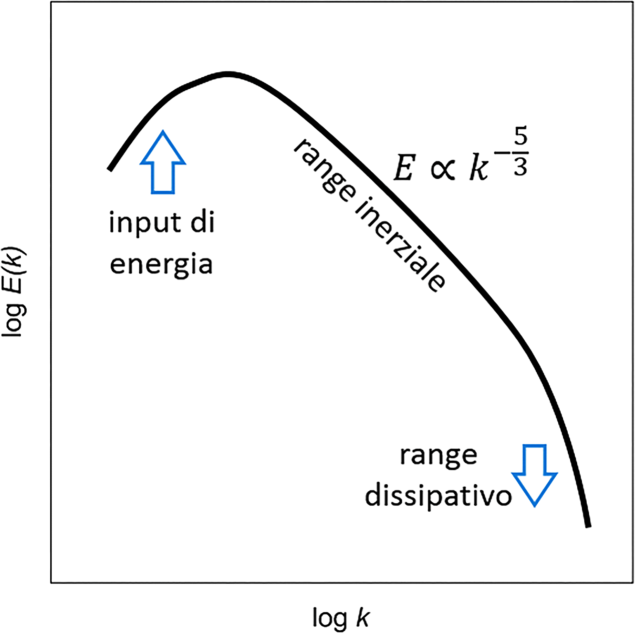
\includegraphics[scale=0.3]{609078_1_It_6_Fig6_HTML.png}
\end{center}

\newpage

\chapter{Dischi di Accrescimento}

In astrofisica si parla di accrescimento ogni volta che un oggetto compatto (e.g. buco nero, nana bianca), circondata da un gas, accresce la sua massa grazie alla caduta del gas verso l'oggetto compatto. \\


Si tratta di un processo che è rilevante in moltissimi ambiti dell'astrofisica, a partire dai buchi neri, alle stelle di neutroni, ed anche fino ad un certo punto per i dischi di saturno. In effetti, la famosa immagine del buco nero Messier 87, del 2019, che riportiamo per completezza, non è effettivamente l'immagine del buco nero, perchè questo non emette radiazione (se non quella di Hawking), ma è una foto del suo disco di accrescimento.

\vspace{1cm}
\begin{center}
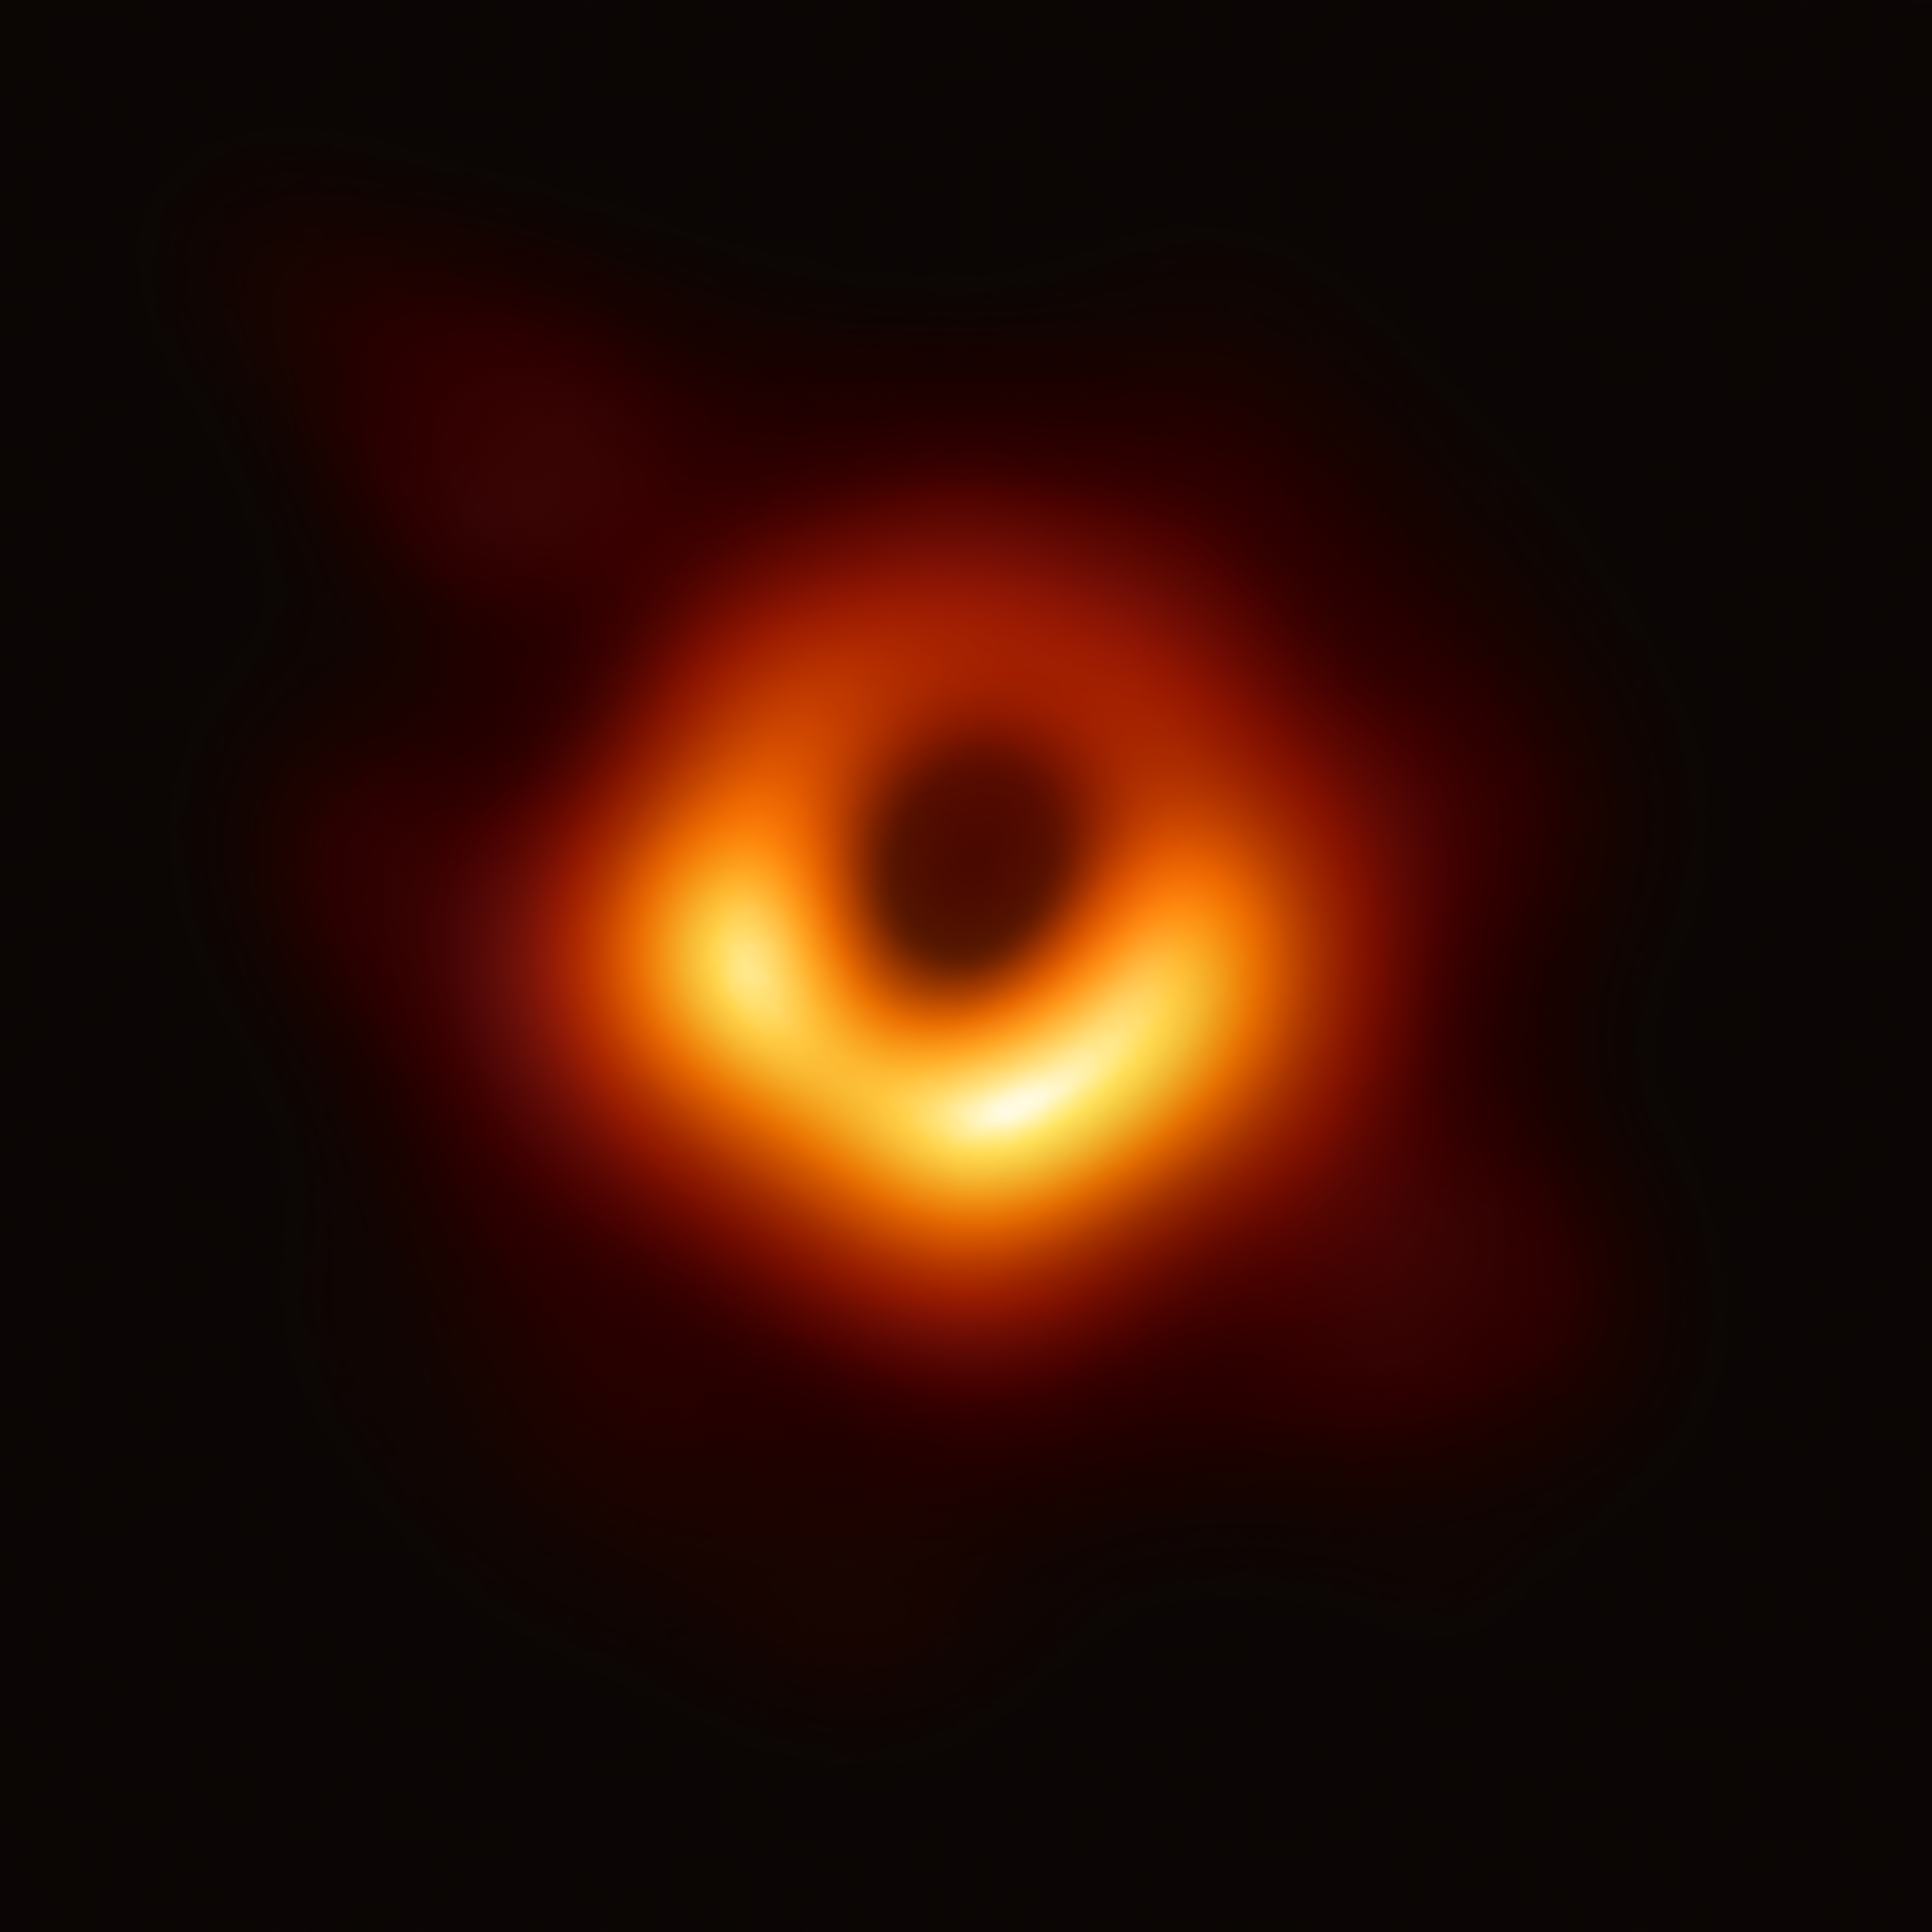
\includegraphics[scale = 0.04]{Black_hole_-_Messier_87_crop_max_res.jpg}
\end{center}
\vspace{1cm}

\section{Accrescimento sferico}

Per cominciare, considereremo un fluido con simmetria sferica. considereremo un fluido inviscido. Scriviamo dunque l'equazioni per tale fluido se in \(r=0\) è presente un corpo puntiforme, di massa \(M\): 
Cominciamo dall'equazione di continuità: 

\begin{align}
    \frac{\partial \rho}{\partial t} + \frac{1}{r^2}\frac{\partial}{\partial r}(r^2u\rho) =0
\end{align}

Nel caso stazionario, questa si riduce ad essere 
\begin{align}
    \frac{\partial}{\partial r}(r^2u\rho) =0 \implies 4\pi r^2 u\rho = \text{cost.} 
\end{align}

D'altra parte, osserviamo che \( 4\pi r^2 u\rho\) è il flusso di massa che attraversa un guscio sferico di raggio \(r\). Ma questo non è altro che il tasso di accrescimento della mia massa: 

\begin{align}
    \dot{M} =  4\pi r^2 u\rho = \text{cost.}
\end{align}

Ora pensiamo ad Eulero: 
\begin{align}
    \frac{\partial u}{\partial t} + u\frac{\partial u}{\partial r} = -\frac{1}{\rho}\frac{\partial p}{\partial r} - \frac{GM}{r^2}
\end{align}

E nel caso stazionario
\begin{align}
    u\frac{\partial u}{\partial r} = -\frac{1}{\rho}\frac{\partial p}{\partial r} - \frac{GM}{r^2}
\end{align}

Ricordando che \(c_s^2 = \frac{\partial p}{\partial \rho}\), possiamo scrivere
\begin{align}
    u^2 \frac{d}{dr}\ln{u} = -c_s^2 \frac{d}{dr}\ln\rho - \frac{GM}{r^2}
\end{align}

Ora possiamo prendere il logaritmo della equazione di continuità e derivare rispetto al raggio: 

\begin{align}
    \frac{d}{dr}\ln u + \frac{d}{dr}\ln\rho +  \frac{2}{r} = 0 \implies \frac{d}{dr}\ln\rho = -\frac{d}{dr}\ln u - \frac{2}{r}
\end{align}

Sostituendo ancora in Eulero troviamo 
\begin{align}
    (u^2- c_S^2)\frac{d}{dr}\ln u = \frac{2c_s^2}{r}\left(1 - \frac{GM}{2c_s^2r} \right)
\end{align}

Che è un'equazione interessante, perchè noi siamo interessati alle soluzioni t.c. 
\begin{enumerate}
    \item \(u(+\infty)=0\), cioè a distanza infinita dalla massa il fluido non sente l'attrazione verso questa
    \item per \(r\rightarrow 0\), ipotizziamo che la velocià debba seguire la forza di gravità, e quindi divergere come \(1/r\). 
\end{enumerate}

Dunque è chiaro che, per continuità, vi sarà certamente un raggio, che chiamiamo \(r_s\), dove varrà \(u(r_s) = c_s\). In particolare, \(r_s\) è detto \emph{punto sonico}, perchè è il punto oltre il quale il fluido diventa supersonico. \\

Il punto sonico è facile da trovare, perchè il lato destro dell'equazione si annulla e potremo scrivere

\begin{align}
    1 - \frac{GM}{2c_s^2r_s} = 0 \implies r_s = \frac{GM}{2c_s^2}
\end{align}

In effetti, questa equazione per \(r_s\) è in realtà incompleta, perchè manca l'informazione su \(c_s = c_s(r)\). Non possiamo supporre in particolare che \(c_s\) sia costante per ogni raggio. \\
Abbiamo menzionato che noi siamo interessati alle soluzioni che hanno velocità nulla all'infinito, ma queste non sono l'unica classe di soluzioni. In effetti, non abbiamo mai detto che la quantità costante \(r^2\rho u\) debba essere per forza positiva: possiamo applicare questa teoria anche ai venti solari, cioè alle particelle emesse dalle stelle, che in effetti possono avere due comportamenti, in base alla loro velocità di emissione: 

\begin{enumerate}
    \item sono \emph{trans-soniche}: vale \(u(r_s) =c_s\), e hanno una velocità monotona crescente. 
    \item sono \emph{subsoniche}: non hanno abbastanza energia per raggiungere la velocità del suono. D'altra parte, per \(r =r_s\) il lato destro dell'equazione si annulla, e dunque \(r_s\) deve essere un massimo della velocità.  
\end{enumerate}

Da adesso in poi, supponiamo che valga \(p = \mathcal{K}\rho^\gamma\). Questo ha come conseguenza che vale 

\begin{align}
    \frac{1}{\rho}\frac{\partial p}{\partial r} = \gamma \frac{P}{\rho^2}\frac{d\rho}{dr} = \gamma \mathcal{K}\rho^{\gamma-2}\frac{d\rho}{dr} = \frac{\gamma\mathcal{K}}{\gamma -1}\frac{d}{dr}\rho^{\gamma -1}
\end{align}

Che ci permette di scrivere l'equazione di Eulero come 
\begin{align}
    \frac{d}{dr}\left(\frac{1}{2}u^2\right) = -\frac{d}{dr}\left(\frac{\mathcal{K}\gamma}{\gamma -1}\rho^{\gamma -1}\right) + \frac{d}{dr}\left(\frac{GM}{r}\right)
\end{align}

Dunque abbiamo un'altra quantità costante, che notando che vale 
\begin{align}
    c_s^2 = \frac{dp}{d\rho} = \gamma \mathcal{K}\rho^{\gamma -1}
\end{align}

è data da 
\begin{align}
    \frac{1}{2}u^2 + \frac{c_s^2}{\gamma -1} - \frac{GM}{r} =0
\end{align}

che non è altro che la \emph{legge di Bernoulli}. Poichè questa è costante, posso valutarla ìn qualunque punto. In particolare, notiamo che per \(r \rightarrow \infty\), l'unico pezzo che sopravvive è la velocità del suono all'infinito, che denotiamo \(c_\infty = c_s(r \rightarrow \infty)\). Possiamo dunque legare questa alla velocità del suono se valutiamo la legge di Bernoulli al punto sonico: 

\begin{align}
    \frac{c_\infty}{\gamma -1}= \frac{1}{2}c_s^2 + \frac{c_s^2}{\gamma -1} - 2c_s^2 \implies c_s^2 = c_\infty^2 \frac{2}{5 - 3\gamma}
\end{align}

In particolare, l'equazione diverge per \(\gamma = 5/3\), che è un valore di \(\gamma\) interessante, perchè corrisponde ad un fluido monoatomico. Di fatto, questo vuol dire che un fluido monoatomico non è mai trans-sonico. Possiamo usare l'equazione anche per ottenere il rapporto fra \(\rho_\infty, \rho(r_s)\), dato da 

\begin{align}
    \left(\frac{\rho(r_s)}{\rho_\infty}\right)^{\gamma -1} = \frac{c_s^2}{c_\infty^2} \implies \rho(r_s) = \rho_\infty \left(\frac{2}{5-3\gamma}\right)^{\frac{1}{\gamma -1}}
\end{align}

Che possiamo inserire nel tasso di accrescimento: 
\begin{align}
    \dot{M} = 4\pi r^2 u \rho = 4\pi r_s^2 \rho(r_s) = f \frac{(GM^2)\rho_{\infty}}{c^3_{\infty}}
\end{align}


Che è noto come \emph{accrescimento di Bondi}. In effetti, vi è anche un altro tipo di tasso di accrescimento che è calcolabile analiticamente, nel caso di un oggetto massiccio che si muove in una nube, con velocità relativa \(v_\infty\). Questo è noto come \emph{accrescimento di Hoyle}, ed è dato da

\begin{align}
    \dot{M} = \frac{4\pi (GM)^2\rho_\infty}{v_\infty^3}
\end{align}

Nel caso misto, non vi è una soluzione analitica, ma si può fare una interpolazione dei due effetti, che solitamente è data da 

\begin{align}
    \dot{M} = \frac{4\pi (GM)^2\rho_\infty}{(v_\infty^2 + c_\infty^2)^{3/2}}
\end{align}

\section{Gas con momento angolare}

La trattazione della sezione precedente, vale per un gas in simmetria sferica, in particolare con momento angolare nullo. In molti casi però il gas ha un momento angolare rilevante. In particolare, questo caso rompe la simmetria sferica e la teoria precedente non vale più. Prima di scrivere le nuove equazioni e considerare in dettaglio la dinamica ed il tasso di accrescimento, vediamo alcuni aspetti qualitivativi. 

\subsection{Aspetti qualitivativi}

Consideriamo, come nel caso precedente, una nube di gas, con al centro un oggetto massiccio, di massa \(M\). \\
Prendiamo un sistema di riferimento cilindrico, \(R, \phi, z\), e supponiamo che il gas abbia un momento angolare non-nullo, \(\vec{\ell} = \ell \hat{z}\). Il gas allora subirà l'effetto di due forze, la forza di gravità e la forza centrifuga: 

\begin{align}
    F = -\frac{GM}{r^2}\hat{r} + \frac{v^2}{r}\hat{R}
\end{align}

Dove \(\vec{r}\) abbiamo indicato il vettore distanza dalla massa \(M\), mentre \(R\) è il raggio cilindrico come già specificato. \\
Ora, possiamo decomporre il vettore \(r\) in una componente lungo \(R\), ed in una componente lungo \(z\): in particolare la seconda, visto che non esistono altre forze che possono contrastarla, portano alla formazione di un disco (spesso sottile) lungo la direzione \(z\). \\

Ci chiediamo in quale regione questo accada ed in quale regione io posso considerare l'approssimazione di acresscimento sferico. Se supponiamo che il momento angolare \(\vec{\ell}\) si conservi (cioè supponiamo di essere in un caso di momento torcente nullo), allora possiamo scrivere il bilancio delle due forze in termini di sole quantità conservate: 

\begin{align}
    F = -\frac{GM}{R^2} + \frac{v^2}{R} = -\frac{GM}{R^2} + \frac{\ell^2}{R^3}
\end{align}

Il punto in cui la forza si annulla è detto \emph{raggio di circolarizzazione}, ed è dato da 

\begin{align}
    R_c = \frac{\ell^2}{GM}
\end{align}

In particolare, osserviamo che 
\begin{enumerate}
    \item \(R > R_c\) \\
    Il sistema può essere descritto in buona approssimazione come accrescimento sferico.
    \item \(R < R_c\) \\
    Il sistema tende ad schiacciarsi in un disco, per l'effetto della barriera centrifuga. Di fatto, il sistema si mette nella configurazione di minima energia potenziale che può ottenere mantenendo costante il momento angolare, che sono le orbite circolari (questo è proprio il motivo del nome). 
\end{enumerate}

\ex{Dimensioni tipiche di una nube molecolare}{
    Dati sperimentali mostrano come tipicamente si ha che, per una nube molecolare, 

    \begin{align}
        R_{\text{core}} \simeq 1 \, \text{Pc} \, (= 3\cdot 10^{18}cm), \quad \Omega_{\text{core}} \simeq 10^{-14}/10^{-13} \, \text{s}^{-1}
    \end{align}

    Da questi possiamo stimare che valga
    \begin{align}
        R_c \simeq (10^2/10^4)\left(\frac{M}{M_s}\right) \, \text{au}
    \end{align}

    Che è un raggio dell'ordine (o di poco superiore) della grandezza del sistema solare. \\

    Questo rivela che lo studio dell'accrescimento per \(R < R_c\) è fondamentale, perchè ad esempio è rilevante per la formazione stellare. 
}

Ora, se il gas rimanesse su orbite circolari mantenendo costante il suo momento angolare non cadrebbe sulla massa \(M\) e non vi sarebbe accrescimento. Di fatto, vi è una forza dissipativa che agisce (in modo secolare) per diminuire il momento angolare, che è data dalla \emph{viscosità}. In effetti, secondo la legge di keplero, il gas si muove con una velocità angolare data da 

\begin{align}
    \Omega_k^2 = \frac{GM}{R^3}
\end{align}

ed in particolare le zone di gas più vicine si muovono con velocità angolare più alta rispetto alle zone più esterne. Questo porta ad uno strisciamento, che permette l'esistenza di una forza di taglio. \\

Chiamiamo dunque \(t_{\nu}\) il \emph{tempo scala viscoso}, che assumiamo per ipotesi essere molto più grande del periodo delle orbite, ovvero 

\begin{align}
    \Omega t_{\nu} >> 1
\end{align}

L'effetto della viscosità è quello di spostare verso l'interno gli elementi più interni, e verso l'esterno gli elementi più esterni. In effetti, questo bilancio è sempre a favore della caduta verso l'interno, così che vi sia sempre accrescimento. Possiamo vederlo facilmente se consideriamo due anelli di gas, a raggi \(R_1 < R_2\), che si scambiano tra di loro del momento angolare: 

\begin{align}
    \Delta J = \delta M_1 \sqrt{GM R_1} = \delta M_2 \sqrt{GMR_2}
\end{align}

Da cui si ottiene  

\begin{align}
    \frac{\Delta M_1}{\Delta M_2} = \left(\frac{R_1}{R_2}\right)^{1/2} > 1
\end{align}

Così che vediamo che si è spostata più massa verso l'interno che verso l'esterno. 

Un'altra importante questione riguarda il \emph{rilascio di energia} durante l'accrescimento. In particolare, l'energia di ciascuna orbita circolare (per unità di massa), è data da \(\eps = -GM/(2R)\), e dunque il rilascio di energia dall'infinito fino ad un raggio minimo \(R_{min}\) è dato da 

\begin{align}
    \eps = \eps(\infty) - \eps_{min} = \frac{GM}{2R_{min}}
\end{align}

Da cui posso ricavare la luminosità: 
\begin{align}
    L = \dot{M}\Delta \eps = \frac{GM \dot{M}}{2R_{min}}
\end{align}

Quando ho a che fare con un buco nero, posso identificare \(R_{min} = R_{isco}\), ovvero il raggio dell'ultima orbita circolare stabile. Vale in particolare che 

\begin{align}
    R_{isco} = \xi \frac{GM}{c^2}
\end{align}

Dove \(\xi = 6\) per il buco nero di Swartschild, \(\xi = 1\) per un buco nero di Kerr per un moto progrado, \(\xi = 9\) per un moto retrogrado sempre per un buco nero di Kerr. \\

In particolare possiamo scrivere che 
\begin{align}
    L = \eta \dot{M}c^2, \quad \eta = \frac{1}{2\xi}
\end{align}

Osserviamo che \(\eta\) indica la frazione dell'energia a riposo del gas che viene convertita in radiazione nel processo di accrescimento. Notiamo che è molto alta (nel caso di Kerr progrado si ha \(eta =0.5\)). Per dare una idea di quanto è grande, confrontiamolo con l'efficacia della fusione nucleare: 

\begin{align}
    \eta_{fus} = \frac{4m_p - m_{He}}{4m_p} = 0.007
\end{align}

In effetti, l'accrescimento di un buco nero è di molto il processo di conversione di energia più efficace nell'intero universo. \\

Uno potrebbe pensare che, siccome aumentando \(dot{M}\) a piacere, potrebbe avere una luminosità \(L\) arbitrariamente grande. Questo in realtà non è possibile, perchè vale il limite di Eddington, dove in pratica la pressione dei fotoni diventa talmente grande da essere confrontabile con la forza di gravità, e non vi è più accrescimento. \\

Per avere un idea di quando avviene questo effetto, dobbiamo avere una idea di quanto valga la pressione dei fotoni. Se scriviamo questa come il flusso di quantità di moto troviamo che 

\begin{align}
    P_{rad} = \frac{L}{4\pi r^2 c}
\end{align}

Perchè ci sia accrescimento deve valere \(F<0\), ovvero che 
\begin{align}
    -\frac{GM m_p}{r^2} + \frac{L \sigma_T}{4\pi r^2 c} < 0
\end{align}

dove abbiamo considerato la forza agente su una coppia legata protone-elettrone. \\

Deve allora valere 

\begin{align}
    L < L_{edd} = \frac{4\pi c m_p GM}{\sigma_T} = 1.26 \cdot 10^{38} \, \text{erg s}^{-1} \left(\frac{M}{M_s}\right)
\end{align}

Il tasso limite è detto tasso di Eddington, 
\begin{align}
    \dot{M}_{edd} = \frac{4\pi G m_p M}{\eta c \sigma_T}
\end{align}

Che definisce un tempo scala minimo di accrescimento 
\begin{align}
    t_{edd} = \frac{c\sigma_T}{4\pi G m_p} = 4.5 \cdot 10^{8}   \, \text{anni}
\end{align}

\subsection{scrittura delle equazioni}

Per la nostra trattazione, assumeremo una simmetria cilindrica. Questo vuol dire che le equazioni non banali saranno nelle direzioni \(z, R\). In effetti, adesso proveremo che anche le equazioni lungo \(z\) sono banali. \\

Per vedere questo, ricordiamo il risultato per la densità, trovato nel capitolo apposito: 

\begin{align}
    &\rho(z) = \rho_0 e^{-\frac{z^2}{2H^2}}, H = \frac{c_s}{\Omega_k} \quad \text{caso non autogravitante} \\
    &\rho(z) = \frac{\rho_0}{\cosh^2 (z/H)}, H =\frac{c_s}{\pi G \Sigma} \quad \text{caso autogravitante}
\end{align}

Facciamo l'ipotesi di disco \emph{sottile}. Questo vuol dire, ricordando che vale 

\begin{align}
    \frac{H}{R} = \frac{c_s}{\Omega_k R} = \frac{c_s}{v_k}
\end{align}

che stiamo considerando un disco supersonico, ovvero \(v_k >> c_s\), oppure  \(\mathfrak{M} >>1\). In generale, questa è una buona approssimazione per i dischi intorno agli AGN, per cui vale tipicamente \(H/R \approx 10^{-2}/10^{-3}\), e decente per i dischi proto-stellari, in cui tipicamente vale \(H/R \approx 10^{-1}\). 

Per quanto invece riguarda la velocità radiale, ricordando che consideriamo un \emph{accrescimento lento}, dovrà valere

\begin{align}
    v_R = Rt_{\nu}^{-1} << R \Omega_k = c_s
\end{align}

Dunque l'ordinamento corretto delle velocità è dato da 
\begin{align}
    v_R << c_s << v_k
\end{align}

D'ora in poi studieremo la struttura del disco nel piano. Per fare questo introduciamo la densità superficiale \(\Sigma\), che è definita da 

\begin{align}
    \Sigma(R) = \int_{-\infty}^{+\infty}\rho(z, R)dz 
\end{align}

Come definiamo in questo caso il coefficiente \(\nu\)? ricorda che in generale vale \(\nu = \eta/\rho\). Possiamo allora definire

\begin{align}
    <\nu> = \frac{\int \nu \rho dz}{\int \rho dz} = \frac{\int \nu \rho dz}{\Sigma}
\end{align}

cioè in pratica come una media verticale pesata. \\

Possiamo allora cominciare a scrivere le nostre equazioni nelle direzioni radiali: le equazioni che ci interessano sono l'eq. di continuità e di Navier-Stokes: 

\begin{align}
    &\frac{\partial \Sigma}{\partial t} + \frac{1}{R}\frac{\partial}{\partial R}(R\Sigma u_R) = 0 \\
    &\rho\left[\frac{\partial \vec{u}}{\partial t} + (\vec{u}\cdot \vec{\nabla})\vec{u}\right] = -\vec{\nabla}p + \vec{\nabla} \cdot \vec{\vec{\sigma}} - \rho \vec{\phi}
\end{align}

Concentriamoci sulla NS. In direzione radiale, la prima parte è nulla, perchè la velocità è tipicamente kepleriana e diretta in direzione azimutale. D'altra parte, nelle forze dovremo anche aggiungere una accelerazione centrifuga, così che in generale scriveremo 

\begin{align}
    \frac{u^2_\phi}{R} = \frac{1}{\rho}\frac{dP}{dR} + \frac{GM}{R^2}
\end{align}

(anche il contributo delle forze viscose è nullo perchè abbiamo solo sheer viscosity). Ci chiediamo allora come è fatta in generale la derivata della pressione rispetto al raggio. Tipicamente i dischi sono \emph{localmente isotropi}, ovvero vale 

\begin{align}
    P(R) = c^2_s (R)\rho(R)
\end{align}

Sostituiamo allora, scrivendo anche l'accelerazione di gravità in termini della velocità kepleriana, e troviamo 

\begin{align}
    u_\phi^2 = v_k^2 +c_s^2 \frac{d\ln P}{d\ln R}
\end{align}

dunque, nell'ipotesi di disco sottile, vale che \(u_\phi \approx v_k\). Se invece vogliamo fare dei calcoli più dettagliati ad esempio per un disco protostellare, dovremo considerare che 

\begin{align}
    u_\phi^2 = v_k^2 \left[1 + \left(\frac{H}{R}\right)^2 \frac{d\ln P}{d \ln R}\right]
\end{align}

Tipicamente, questa correzione è negativa perchè la pressione decresce col crescere di \(R\). 

In effetti, il calcolo si può estendere anche per \(z \neq 0\). In particolare in questo caso si avrebbe che 

\begin{align}
    u^2_\phi = v_k^2\left[1 - \gamma \left(\frac{H}{R} \right)^2 - q\left(1 - \frac{1}{\sqrt{1 + z^2/R^2}} \right)\right] 
\end{align}

dove abbiamo indicato \(\gamma = \frac{d\ln P}{d\ln R}, q = \frac{d\ln T}{d\ln R}\). In particolare, se il disco è \emph{isotermo}, questo vuol dire che \(q=0\), e la velocità è indipendente dalla \(z\). Questo vuol dire che il disco ruota su cilindri. In effetti questa è una conseguenza di un teorema generale, dovuto a Poincarè, che afferma che in equilibrio idrostatico, un gas isotermo \emph{deve} ruotare su cilindri. \\

Invece cosa succede quando l'autogravità diventa non trascurabile? Chiaramente, questo dipende da come è fatta in quel caso \(d\phi/dR\). In effetti, sono noti almeno un paio di risultati analitici: 

\begin{enumerate}
    \item \(\Sigma(R) = \Sigma_0 e^{-R/R_0}\),in questo caso \(v^2_{\text{disc}} = R\frac{d\phi}{dR}\) è analitica, nel senso che può essere scritta come somma di funzioni di Bessel. All'infinito decresce come \(R^{-1}\). 
    \item \(\Sigma(R) = \frac{\Sigma_0R_0}{R}\), detto anche disco di Metsel, in questo caso la velocità è costante, ed in particolare vale \(v^2_{\text{disc}} = 2\pi G\Sigma_0 R_0\). 
\end{enumerate}


In generale, le correzioni dell'autogravità sono dell'ordine \(M_{\text{disc}}/M_{*}\). Ma nei dischi sottili invece sono dell'ordine di

\begin{align}
    \left(\frac{M_{\text{disc}}}{M_*} \right)\left(\frac{R}{H}\right)
\end{align}

e quindi in diverse situazioni possono essere rilevanti. \\

Scriviamo ora le equazioni di Navier-Stokes in direzione azimutale. Per farlo, ricordiamo la forma del tensore dello stress: 

\begin{align}
    \sigma_{ij} = \eta \left[\frac{\partial u_i}{\partial x_j} + \frac{\partial u_j}{\partial x_i} - \frac{2}{3}(\vec{\nabla}\cdot \vec{u})\delta_{ij}\right]
\end{align}

Passando in coordinate cilindriche, vale 

\begin{align}
    \sigma_{R\phi} = \sigma_{\phi R} = \eta R \frac{d\Omega}{dR}
\end{align}


e definiamo allora 

\begin{align}
    T_{R\phi} = \int \sigma_{R\phi} = \nu \Sigma R \frac{d\Omega}{dR}
\end{align}

dove nell'ultima uguaglianza abbiamo usato l'ipotesi di disco sottile. \\

Dunque, le equazioni di NS in direzione azimutale si possono scrivere 

\begin{align}
    \frac{\partial }{\partial t}(\Sigma R u_\phi) + \frac{1}{R}\frac{\partial}{\partial R}(R u_R \Sigma R u_\phi) = \frac{1}{R}\frac{\partial}{\partial R}(R^2 T_{R\phi}) = \frac{1}{R}\frac{\partial}{\partial R}(\nu \Sigma R^2 \Omega)
\end{align}

Notiamo che l'equazione ha un aspetto familiare: è una legge di conservazione! dice che la variazione nel tempo di una quantità, in questo caso di \(\Sigma R u_\phi\), che riconosciamo essere la densità del momento angolare, è uguale alla diveergenza di un tensore più un termine dissipativo, dovuto alla presenza delle forze viscose. Interpretiamo dunque questa equazione come l'equazione per il bilancio del momento angolare del disco.  \\

Ci occupiamo ora di riscrivere l'equazione in una forma ancora più interessante: usando solamente la regola di derivazione del prodotto otteniamo

\begin{align}
    R u_{\phi} \frac{\partial \Sigma}{\partial t} + R\Sigma \frac{\partial u_\phi}{\partial t} + Ru_\phi \frac{1}{R}\frac{\partial}{\partial R}(Ru_\phi \Sigma) + \frac{Ru_\phi}{R}\Sigma \frac{\partial}{\partial R}(Ru_\phi) = \frac{1}{R}\frac{\partial}{\partial R}(\nu \Sigma R^3 \Omega')
\end{align}

Ora l'espressione può essere semplificata perchè \(\partial_t u_\phi = 0\), in quanto si tratta semplicemente della velocità kepleriana in buona approssimazione, ed invece il primo ed il terzo termine si annullano in virtù dell'equazione di continuità. Non ci resta allora che considerare

\begin{align}
    R u_R \Sigma = \frac{\frac{\partial }{\partial R}(\nu\Sigma R^3 \Omega')}{\frac{\partial }{\partial R}(Ru_\phi)}
\end{align}


che possiamo sostituire nell'equazione di continuità: 

\begin{align}
    \frac{\partial \Sigma}{\partial t} = -\frac{1}{R}\frac{\partial }{\partial R}\left[\frac{1}{(R^2\Omega)'}\frac{\partial}{\partial R}(\nu \Sigma R^3 \Omega')\right]
\end{align}

L'eq. è generale, ma se scriviamo \(\Omega = \Omega_k\), allora \(\Omega' = -(3/2)\Omega\), \((R^2\Omega)' = (1/2)\Omega R\). Dunque potremmo riscrivere

\begin{align}
    \frac{\partial \Sigma}{\partial t} = \frac{3}{R}\frac{\partial }{\partial R}\left[\frac{R^{1/2}}{(GM)^{1/2}}\frac{\partial }{\partial R}(\nu\Sigma (GM)^{1/2}R^{1/2})\right]
\end{align}

semplificando, 

\begin{tcolorbox}[colback=myg!15, colframe=black, boxrule=1pt]
\begin{align}
    \label{eq:evolution_disk}
    \frac{\partial \Sigma}{\partial t} = \frac{3}{R}\frac{\partial }{\partial R}\left[R^{1/2}\frac{\partial }{\partial R}(\nu \Sigma R^{1/2})\right]
\end{align}
\end{tcolorbox}

questa è l'equazione \emph{fondamentale} per l'evoluzione temporale dei dischi di accrescimento. Si noti in particolare che ha la struttura di una equazione di \emph{diffusione}. Questo diventa ancora più evidente se si passa alla variabile \(y = R^{1/2}\), allora in quel caso si ha che 

\begin{align}
    \frac{\partial \Sigma}{\partial t} \propto \frac{\partial}{\partial y^2}(\nu \Sigma \ldots )
\end{align}

Questo è importante perchè ci dice che la diffusione (e quindi l'accrescimento) avviene su tempi scala

\begin{align}
    t_{\nu} \propto \frac{R^2}{\nu} >> \Omega^{-1}
\end{align}

In particolare, questo vuol dire che, deducendo l'ordine di grandezza della velocità radiale 

\begin{align}
    u_R = \frac{1}{R\Sigma}\frac{\frac{\partial}{\partial R}(\nu\Sigma R^2 \Omega')}{(R^2\Omega)'} \approx \frac{\nu \Omega R}{\Omega R^2} = \frac{\nu}{R}
\end{align}

Troviamo che deve valere 

\begin{align}
    \frac{u_\phi R}{\nu} >> 1
\end{align}

così che le condizioni di disco sottile e di accrescimento lento sono sinteticamente assicurate dalle due condizioni 

\begin{align}
    \mathfrak{M} >> 1, \quad \text{Re} >> 1
\end{align}

\subsection{Soluzioni delle equazioni}

L'equazione per l'evoluzione temporale dei dischi di accrescimento \ref{eq:evolution_disk} è in generale complicata da risolvere, perchè la viscosità può dipendere sia dalla densità superficiale, sia dal raggio del disco, ovvero \(\nu = \nu(\Sigma, R)\). D'altra parte, è possibile determinare delle soluzioni in forma analitica, nel caso speciale in cui valga \(\nu(R) = R^b\). 

In particolare, il caso in cui \(b=0\), ovvero \(\nu = \text{const.}\), è semplice da risolvere, trovando con la trasformata di Fourier la funzione di green. Questo vuol dire trovare la soluzione se la configurazione iniziale è data da 

\begin{align}
    \Sigma(R, t=0) = \frac{m}{2\pi R_0}\delta(R-R_0)
\end{align}

ovvero un anello di raggio \(R_0\), con massa totale \(m\). In particolare, si trova che la soluzione è data da 

\begin{align}
    \Sigma(X, \tau) = \frac{m}{\pi R_0^2}\frac{X^{-1/4}}{\tau}\exp\left(-\frac{(1+x^2)}{\tau} \right)I_{1/4}\left(\frac{2X}{\tau}\right)
\end{align}

Dove abbiamo definito le variabili riscalate \(X = R/R_0\), \(\tau = 12\nu t/R_0^2\), mentre \(I\) indica la funzione di Bessel modificata.\\

Notiamo una differenza di un fattore \(12\) nel tempo scala di questa soluzione, e di quello tipico che ci aspettiamo da una equazione diffusiva. Questo è dovuto ai gradienti molto \emph{ripidi} della configurazione iniziale, che portano ad una diffusione più rapida del normale. \\

Un'altra soluzione è nota come soluzione \emph{self-similar}, ed è valida per \(b<2\). A titolo di esempio, riportiamo la soluzione nel caso \(b=1\), 

\begin{align}
    \Sigma(R, t=0) = \frac{C}{3\pi \nu(R)}e^{-R/R_1}, \implies \Sigma(R, T) = \frac{CT^{-3/2}}{3\pi \nu(R)}e^{-\frac{R}{TR_1}}
\end{align}

dove abbiamo indicato \(T = 1+ t/t_\nu\), \(t_\nu = R_1^2/(3\nu(R))\).  \\

Quali sono alcune proprietà universali delle soluzioni? L'\emph{allargamento viscoso} sicuramente è una caratteristica generale del problema. \\

In particolare, fissati un certo raggio \(R\), possiamo determinare il flusso di massa: 

\begin{align}
    \dot{M}(R, t) = -2\pi u_r R \Sigma(R, t)
\end{align}

Nel caso self-similar, questo è dato da 

\begin{align}
    \dot{M} = cT^{-3/2}e^{-\frac{R}{TR_1}}\left(1- \frac{2R}{TR_1} \right)
\end{align}

Ora, dalle equazioni, sembrerebbe che il raggio del disco aumenti sempre di più. Questo dipende però dalla definizione che diamo di raggio del disco. Se scegliamo di prendere il raggio del disco come il ragggio dentro al quale sta una certa percentuale della massa, allora il raggio del disco cetramente diminuirà col tempo. 


Rivolgiamo ora la nostra attenzione verso il momento angolare: notiamo che possiamo scrivere 

\begin{align}
    \frac{1}{R}\frac{\partial}{\partial R}(\nu \Sigma R^3 \Omega') = \frac{1}{2\pi R}\frac{\partial \mathcal{L}}{\partial R}, \, \mathcal{L} = 2\pi\nu \Sigma R^3\Omega'
\end{align}

Consideriamo allora due anelli nel disco, con raggi \(R_2 > R_1\), con \(R_2-R_1 = \Delta R << R_1\). Mi posso chiedere quale è il momento torcente netto agente sull'anello. Devo allora integrare la densità di momento torcente: 

\begin{align}
    \frac{dL}{dt} = \int_{R1}^{R_2} 2\pi R \left(\frac{1}{2\pi R}\frac{\partial}{\partial R} \mathcal{L}\right) = \mathcal{L}(R_2) - \mathcal{L}(R_1)
\end{align}

Interpretiamo dunque \(\mathcal{L}\) come il flusso di momento angolare verso l'interno. Notiamo che poichè \(\Omega' <0\), scopriamo una fondamentale proprietà dei dischi: 

\nt{Mentre la massa del disco va verso l'interno, il momento angoalare va verso l'esterno}

Nel caso di soluzioni stazionarie, la condizione \(\partial_t \Sigma =0\) impone che valga 

\begin{align}
    \frac{\partial}{\partial R}(Ru_R \Sigma) = 0 
\end{align}

In particolare, il tasso di accrescimento sarà 

\begin{align}
    \dot{M} = -2\pi R u_R \Sigma = \text{const.}
\end{align}

e il flusso di momento angolare? dall'eq. di bilancio del momento angolare, ovvero dalla NS in coordinate azimutali, per soluzioni statiche deve valere 

\begin{align}
    \frac{\partial}{\partial R}(Ru_R \Sigma R^2 \Omega - \nu \Sigma R^3\Omega') = 0 
\end{align}

In generale, vale 

\begin{align}
    -\frac{\dot{J}}{2\pi} = R^3u_r \Sigma \Omega - \nu\Sigma R^3 \Omega' 
\end{align}

ovvero 

\begin{align}
    \dot{J} = -2\pi R u_R \Sigma \Omega R^2 + 2\pi \nu \Sigma R^3 \Omega' = \dot{M}\Omega R^2 + 2\pi \nu \Sigma R^3 \Omega
\end{align}

Questa formula è importante perchè permette di distinguere due termini che controbuiscono al momento torcente: 

\begin{enumerate}
    \item Il termine di \emph{avvezzione}, proporzionale ad \(\dot{M}\). Questo è dovuto alla massa che viene trasportata. 
    \item Il termine di momento torcente \emph{viscoso}, invece proporzionale a \(\nu\). Corrisponde alla quantità \(\mathcal{L}\) prima determinata. 
\end{enumerate}

i due termini sono opposti, come si vede esplicitando \(\Omega' = -(3/2)(\Omega/R)\). In questo caso, l'eq. completa diventa 

\begin{align}
    \dot{J} = \dot{M}\Omega R^2 - 3\pi \nu \Sigma \Omega R^2
\end{align}

Lungo tutta questa discussione, abbiamo assunto che \(\Omega = \Omega(R)\) fosse data dalla frequenza kepleriana, ovvero in particolare \(\Omega(R) \propto R^{-3/2}\). Questo però non può essere la vera velocità del disco nel caso in cui questo sia attorno ad un oggetto compatto, ad esempio una stella: necessariamente ad \(R_*\) la velocità del disco dovrà coincidere con la velocità di rotazione della stella, che chiaramente sarà finita. Tipicamente, la forma di \(\Omega(R)\) in una situazione realistica è la seguente: 

\begin{enumerate}
    \item Per \(R >> R_*\), la velocità è in buona approssimazione data dalla frequenza kepleriana. Si ha quindi \(\Omega \propto R^{-3/2}\). 
    \item Nelle vicinanze di \(R_{*}\), tipicamente esiste una distanza \(b\), t.c. \(\Omega\) abbia un massimo in \(\Omega(R_* + b)\), che tipicamente è maggiore della velocità della stella. Nella regione \([R_*, R_* +b]\), detta anche \emph{strato limite}, \(\Omega\) è dunque una funzione crescente della distanza. 
\end{enumerate}


In particolare, possiamo sfruttare il fatto che valga \(\Omega'(R_* + b) = 0\), e trovare che in quel punto varrà 

\begin{align}
    \dot{J} = \dot{M}\Omega(R_* + b)(R_* + b)^2 \approx \dot{M}\Omega(R_*)R_*^2 = \dot{M}(GMR_*)^{1/2}
\end{align}


Sostituendo questa relazione nell'equazione iniziale, otteniamo 

\begin{align}
    \dot{M}(GM R_*)^{1/2} = (GM R_*)^{1/2}(\dot{M} - 3\pi \nu \Sigma) \implies 3\pi \nu \Sigma = \dot{M}\left( 1 - \sqrt{\frac{R_*}{R}} \right)
\end{align}

Questa è una relazione di grande importanza, ed in particolare se \(R >> R_*\), allora troviamo che deve valere 

\begin{align}
    \dot{M} = 3\pi \Sigma \nu
\end{align}

Questo ragionamento è stato fatto se l'oggetto che accresce ha una superficie fisica. D'altro canto, tutte queste considerazioni sono valide anche per i buchi neri, a patto di sostituire il raggio della stella con il raggio dell'ultima orbita circolare stabile. \\

Come ultima osservazione, se riscriviamo 

\begin{align}
    \Sigma = \frac{\dot{M}}{3\pi \nu}
\end{align}

e la confrontiamo con la condizione iniziale della self-similar, (che \emph{non} è una soluzione statica)

\begin{align}
    \Sigma(t=0) = \frac{C}{3\pi \nu}e^{-R/R_1}
\end{align}

Ci rendiamo conto che la dinamica del disco è dovuta allo smorzamento esponenziale della densità superficiale, che non permette al disco di prendere abbastanza momento angolare dall'esterno per essere stabile. 

\subsection{Energia nei dischi}

Essendo dei sistemi viscosi, i dischi dissipano energia. Calcoliamo allora il lavoro delle forze viscose: 

\begin{align}
    P_{visc} = \frac{\partial \mathcal{L}}{\partial R}(\Delta R)\Omega = \Delta R \left(\frac{\partial}{\partial R} (\mathcal{L}\Omega) - \mathcal{L}\Omega'\right)
\end{align}

Il primo termine è un trasporto viscoso di energia, il secondo è il termine di disspiazione che cercavamo. Poichè questa è la potenza dissipata sull'anello, se dividiamo per l'area dell'anello troviamo la potenza dissipata per \emph{unità di superficie} (per convenzione positivo): 

\begin{align}
    D(R) = \frac{\mathcal{L}\Omega' \Delta R}{2\pi R \Delta R} = \frac{\mathcal{L}\Omega'}{2\pi R} = \nu\Sigma (R\Omega')^2
\end{align}

questa quantità è nota come \emph{tasso di dissipazione}

\ex{\(D(R)\) per dischi kepleriani}{

    Ricorda che per dischi kepleriani vale \(\Omega(R) = \frac{(GM)^{1/2}}{R^{3/2}} \implies \Omega' = -\frac{3}{2}\frac{(GM)^{1/2}}{R^{5/2}}\), da cui leggiamo 

    \begin{align}
        D(R) = \frac{9}{4}\nu\Sigma \frac{GM}{R^3}
    \end{align}
}

\ex{\(D(R)\) per dischi kepleriani statici}{

    Se un disco oltre ad essere kepleriano è anche statico, sappiamo che deve valere 

    \begin{align}
        \nu\Sigma = \frac{\dot{M}}{3\pi}\left(1 - \sqrt{\frac{R_*}{R}} \right)
    \end{align}

    così che scriveremo 

    \begin{align}
        D(R) = \frac{3}{4\pi}\frac{GM\dot{M}}{R^3}\left(1-\sqrt{\frac{R_*}{R}} \right)
    \end{align}
}

Sapendo quanta energia viene dissipata per unità di tempo e di superficie, possiamo ottenere la \emph{luminosità} del disco: ancora per un disco kepleriano e statico, 

\begin{align}
    L_{disc} = \int_{R_*}^{+\infty}2\pi R D(R) dR = \int_{R_*}^{+\infty}\frac{3}{2}\left(\frac{GM\dot{M}}{R^2}\right)\left(1 - \sqrt{\frac{R_*}{R}} \right) = \frac{1}{2}\frac{GM\dot{M}}{R_*}
\end{align}

A prima vista il risultato potrebbe sembrare strano: in effetti, leggendo dall'integranda avremmo 

\begin{align}
    dE_{disc} = \frac{3}{2}\frac{GM\dot{M}}{R^2}dR
\end{align}

ma, d'altra parte, 

\begin{align}
    d\left(\frac{GM}{R} \right) = -\frac{GM}{R^2}dR
\end{align}

sembra dunque che il disco stia dissipando più energia di quanta ne sta guadagnando! Il fatto è che non stiamo considerando il termine di avviazione, 

\begin{align}
    \Delta E_{visc} &= \Delta R \frac{\partial}{\partial R}(2\pi \nu \Sigma R^3 \Omega \Omega') = -\Delta R \frac{\partial}{\partial R}(3\pi\nu\Sigma R^2\Omega^2) \\
    &= -\Delta R \frac{\partial}{\partial R}\left(\frac{GM\dot{M}}{R} \right) = \Delta R \frac{GM\dot{M}}{R^2}
\end{align}

che è esattamente il pezzo del puzzle che mancava. \\

Per continuare la nostra trattazione dell'energia vorremo considerare la temperatura del disco. Per fare questo facciamo una ipotesi che semplifica notevolmente il problema: supponiamo che il nostro disco sia \emph{otticamente spesso}. Questo in poche parole vuol dire che i fotoni, prima di uscire dal disco interagiscono molte volte. \\

Più formalmente, indichiamo con \(\tau = K \Sigma\) lo spessore ottico, dove \(K\) è l'opacità del mezzo, che in genere dipende dal processo radiativo. Richiedere che il disco sia otticamente spesso vuol dire chiedere che \(\tau >> 1\). \\

Ora il motivo per cui abbiamo fatto questa assunzione è che un mezzo otticamente spesso, in equilibrio termico non è altro che un \emph{corpo nero}. La sua temperatura è allora legata alla potenza emessa da 

\begin{align}
    \mathcal{F}_{rad} = 2\sigma_{SB}T_s^4
\end{align}

all'equilibrio, si avrà un bilancio fra il riscaldamento ed il raffreddamento. Allora dovrà valere 

\begin{align}
    2\sigma_{SB}T_S^4 = \frac{3}{4\pi}\frac{GM\dot{M}}{R^3}\left(1- \sqrt{\frac{R_*}{R}} \right)
\end{align}

dunque l'equazione può essere usata per ricavare la temperatura della \emph{superficie} del disco ad un dato raggio. Ad esempio, se \(R >> R_*\), possiamo dedurre che vale 

\begin{align}
    T_S(R) = T_0 \left(\frac{R_*}{R}\right)^{3/4}, \, T_0 = \left(\frac{3}{8\pi\sigma_{SB}}\frac{GM\dot{M}}{R_*^3} \right)^{1/4}
\end{align}

Ora, quando questa formula è valida? In altre parole, quali sono state le ipotesi che abbiamo fatto per ricavarla? 

\begin{enumerate}
    \item Disco Kepleriano: questa approssimazione è valida nella maggior parte dei casi, perchè vuol dire che sto considerando dischi dove l'autogravità non ha effetti apprezzabili. 
    \item Abbiamo considerato come processo di riscaldamento solamente la viscosità. In effetti, non è detto che questo sia il caso, ad esempio il disco può prendere calore dall'irraggiamento della stella che sta accrescendo. Per questo motivo, si distinguono due tipi di dischi: 
    \begin{enumerate}
        \item dischi \emph{attivi}: il riscaldamento è dominato dalla viscosità
        \item dischi \emph{passivi}: il riscaldamento è dominato dalla stella 
    \end{enumerate}
\end{enumerate}


Come è fatto il profilo di temperatura nel caso di dischi passivi? Varrà \(F_{irr} \approx R^{-2}\). D'altra parte devo considerare anche l'angolo con cui la radiazione della stella colpisce il disco, così che più precisamente varrà 

\begin{align}
    F_{irr} \propto \sin\theta R^{-2} = \frac{R_*}{R}R^{-2} \approx R^{-3}
\end{align}

Si ottiene allora che il profilo di temperatura è dato da 

\begin{align}
    T_S (R) \propto R^{-1/2}
\end{align}

\subsection{Spettro di emissione}

Arrivati a questo punto, siamo pronti a chiederci come è fatto lo spettro della radiazione emessa da un disco di accrescimento. Una domanda ingenua sarebbe la seguente: perchè siamo interessati allo spettro emesso dal disco, se sappiamo che il disco si comporta come un corpo nero, ad una certa temperatura \(T_s\)? Risposta: perchè la temperatura \(T_s = T_s(R)\) è una funzione del raggio, quindi possiamo pensare che ogni cerchio del disco emetta uno spettro di corpo nero alla sua temperatura. Dunque, lo spettro totale è datto dalla somma (o meglio, dall'integrale) dello spettro di corpo nero emesso da ogni cerchio. 

Ricorda che la potenza emessa da un corpo nero ha lo spettro ricavato da Plank, 

\begin{align}
    B_v(T) = \frac{2 h \nu^3}{c^2}\frac{1}{e^{\frac{h\nu}{KT}}-1}
\end{align}

con \(h\) la costante di Plank, \(K\) la costante di Boltzmann. 

\begin{center}
    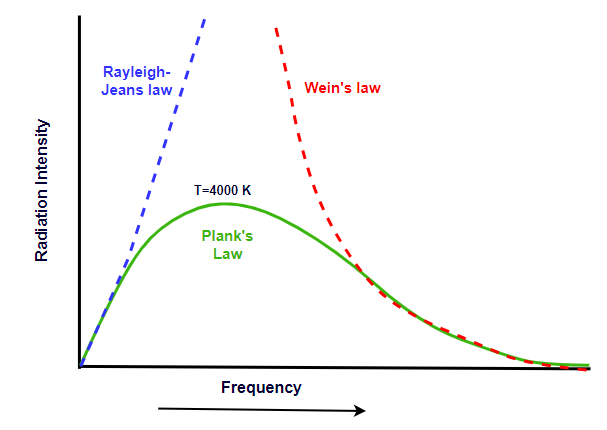
\includegraphics[scale = 0.5]{blackbody-spectrum.png}
\end{center}

La figura mostra lo spettro di radiazione. In particolare, la figura evidenzia anche due regimi dello spettro: 

\begin{enumerate}
    \item \(h\nu << KT\), nel limite di basse frequenze, lo spettro assume la forma di una legge di potenza, in particolare vale 
    \begin{align}
        B_\nu \approx \frac{2\nu^2}{c^2}KT
    \end{align}
    questa è nota come legge di Rayleigh-Jeans. 
    \item \(h\nu >> KT\), nel limite di alte frequenze, lo spettro viene smorzato esponenzialmente e assume la forma asindotica
    \begin{align}
        B_\nu \approx \frac{2h\nu^3}{c^2}e^{-\frac{h\nu}{KT}}
    \end{align}
    questa è invece nota come legge di Wien. 
\end{enumerate}


Dunque, lo spettro del disco sarà invece dato da 

\begin{align}
    F_\nu = \int_{R_{int}}^{R_{ext}} \frac{2h \nu^3}{c^2}\frac{2\pi RdR}{e^{\frac{h\nu}{KT(R)}}-1}
\end{align}

Sfortunatamente, non è possibile risolvere l'integrale completo analiticamente, a causa della dipendenza \(T= T(R)\) che rende l'integrale molto complicato. D'altra parte, possiamo invece indagare lo spettro nelle varie regioni, usando la forma asindotica opportuna della radiazione di Plank. 

\begin{enumerate}
    \item Se \(h\nu << KT_{out}\), allora per tutti i dischi è valida la legge di Rayleigh-Jeans, e possiamo dedurre che 
    \begin{align}
        F_\nu = \int \frac{2\nu^2}{c^2}KT_0 \left(\frac{R}{R_0} \right)^{-q}2\pi R dR \propto \nu^2
    \end{align}
    \item se \(h\nu >> KT_{in}\), allora per tutti i dischi vale la legge di Wien. Possiamo allora ricavare
    \begin{align}
        F_\nu \approx \int \frac{2h \nu^3}{c^2}e^{-\frac{h\nu}{KT(R)}}2\pi R dR = \ldots = e^{-\frac{h\nu}{KT_{in}}}
    \end{align}
    \item La regione intermedia sembra essere per ovvie ragioni la più problematica. In effetti però, possiamo comunque dedurre la forma dello spettro. Scrivo in particolare 
    \begin{align}
        X = \frac{h\nu}{KT} = \frac{h\nu}{KT_0}\left(\frac{R}{R_0} \right)^{q} \propto \nu R^{q}
    \end{align}
    Cambio allora astutamente variabili \(R \rightarrow X\). Poichè \(R \propto (X/\nu)^{1/q}\), il differenziale sarà  \(\frac{dx}{x} = q\frac{dR}{R}\). Troviamo allora che 

    \begin{align}
        F_\nu \propto \int \nu^3 \left(\frac{X}{\nu} \right)^{2/q} \frac{dX}{X} \frac{1}{e^X -1} = \nu^{3-2/q}\int_{X_{in}}^{X_{out}}\frac{X^{2/q -1}}{e^X -1}dX
    \end{align}

    Nota che l'integrale è ancora dipendente da \(\nu\), perchè lo sono gli estremi di integrazione. D'altra parte, se vale sia \(h\nu << kT_{in}\), sia \(h\nu >> kT_{out}\), allora posso in buona approssimazione concludere che 

    \begin{align}
        F_\nu \propto \nu^{3-2/q}\int_{0}^{+\infty}\frac{X^{2/q -1}}{e^X -1}dX \propto \nu^{3-2/q}
    \end{align}
\end{enumerate}


Concludiamo che la forma qualitativa dello spettro emesso deve essere quella raffigurata in figura: 

\begin{center}
    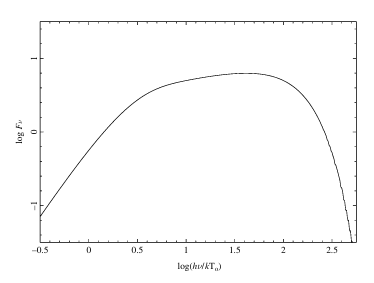
\includegraphics[scale =0.8]{Accretion-disck-power-spectrum.png}
\end{center}

possiamo vederlo in pratica come uno spettro di corpo nero "stiracchiato", ovvero dove più picchi a diverse temperature si sommano. 

Per avere un'idea della scala, tipicamente \(KT_{in}\) per gli AGN è nel range dell'ultra-violetto. 

Torniamo per un momento a considerare le scale temporali del problema. In particolare, ci chiediamo quando ci mette il sistema a raggiungere l'equilibrio termico, rispetto agli altri tempi scala, che ricordiamo essere nell'ordine 

\begin{align}
    t_{dyn} = \Omega^{-1} \approx t_z << t_\nu = R^2/\nu
\end{align}

introduciamo ora una ipotesi sulla viscosità, che fu introdotta da Shakura e Sunyaev. Torneremo su questa e su come si giustifica più avanti: 
\begin{align}
    \nu = \alpha c_s H \implies t_\nu = \frac{R^2}{\alpha c_s H} = \frac{R^2}{c_s \Omega H^2}  = \frac{1}{\alpha}\left(\frac{H}{R} \right)^{-2}\frac{1}{\Omega}
\end{align}

il che mostra ancora una volta come \(t_\nu >> t_{dyn}\). Il numero \(\alpha\) è un parametro adimensionale, minore di 1. \\

Pensiamo allora ai tempi scala termici, che indichiamo con \(t_{th}\). Ricorda che l'energia interna per unità di massa è data da 

\begin{align}
    e = \frac{c_s^2}{\gamma(\gamma -1)}
\end{align}

dunque il tempo scala termico sarà dato da 

\begin{align}
    T_{th} = \frac{\Sigma e}{D(R)} = \frac{c_s^2 \Sigma}{\gamma(\gamma -1)}\frac{1}{\nu\Sigma(R\Omega')^2}
\end{align}

nell'assunzione di un disco kepleriano, 

\begin{align}
    T_{th} = \frac{4}{9}\frac{1}{\gamma(\gamma-1)}\frac{c_s^2}{\nu \Omega^2}
\end{align}

usando infine ancora una volta la formula di Shakura-Sunyaev, troviamo che 

\begin{align}
    t_{th} = \frac{4}{9}\frac{1}{\gamma(\gamma -1)}\frac{t_{dyn}}{\alpha}
\end{align}

Ricordando che \(\alpha < 1\), si ottiene allora che il corretto ordinamento delle scale temporali è dato da 

\begin{align}
    t_{dyn} << t_{th} << t_{\nu}
\end{align}

Ora, nell'ipotesi di disco otticamente spesso, si ha che la temperatura alla superficie, è legata alla temperatura al centro del disco, cioè alla temperatura nel piano equatoriale, da 

\begin{align}
    T_c = T_s \tau^{1/4}
\end{align}

A questo punto, posso legare tutte le proprietà interessanti del disco dalle seguenti equazioni: 

\[
\begin{cases}
    T_s^4 = \frac{3}{8\pi\sigma_{SB}}\frac{GM\dot{M}}{R^3}\left( 1 - \sqrt{\frac{R_*}{R}}\right) \\
    T_c = \tau^{1/4}T_s \\
    c_s^2 = \frac{KT_c}{\mu_{mp}}\\
    \nu = \alpha c_s H \\
    H = c_s\Omega \\
    3\pi \nu \Sigma = \dot{M}\left(1 - \sqrt{\frac{R_*}{R}}\right) 
\end{cases}
\]

Questo sistema fu risolto la prima volta, proprio da Shakura-Sunyaev. Il risultato dei loro calcoli fu che è possibile dividere il disco in 3 zone: 

\begin{enumerate}
    \item La parte più vicina al buco nero ed interna, che è dominata dalla pressione di radiazione e dallo scattering di Thompson 
    \item La parte intemedia, che è dominata dalla pressione del gas e da scattering Thompson 
    \item la parte esterna, che è dominata da pressione del gas + scattering free-free
\end{enumerate}

\subsection{Problema della viscosità/ del trasporto anomalo}

Torniamo allora indietro alla formula che avevamo scritto, ed avevamo anticipato essere stata persa come modello da Shakura-Sunyaev: 

\begin{align}
    \nu = \alpha c_s H
\end{align}

in particolare, calcoliamo la viscosità a livello microscopico, a partire cioè dalle collisioni fra particelle. Ricordiamo allora il ruolo della viscosità nei dischi: 

il tensore degli stress ha una unica componente non nulla, ovvero 

\begin{align}
    T_{R \phi} = \nu\Sigma (R\Omega') = \nu \Sigma \Omega \frac{d\ln\Omega}{d\ln R}
\end{align}

La viscosità è poi direttamente proporzionale al tasso di accrescimento: 

\begin{align}
    \dot{M} = 3\pi \nu \Sigma
\end{align}

Dimensionalmente, una viscosità \(\nu\) è una velocità per una lunghezza. Varrà allora che 

\begin{align}
    \nu \approx \tilde{v}\lambda
\end{align}

con \(\tilde{v} \approx c_s\), e la scala tipica sarà invece circa il cammino libero medio, che è dato da \(\lambda = \frac{1}{n\sigma_{coll}}\), con \(\sigma_{coll}\) la sezione d'urto collisionale. Invece \(n\) è la densità numerica di particelle (in questo caso, molecole), e quindi possiamo scriverla \(n = \rho/\mu_{mp}\). Questo vuol dire che in un fluido collisionale si ha circa 

\begin{align}
    \nu \approx \frac{\mu_{mp}c_s}{\rho \sigma_{coll}} \rightarrow \nu \approx \frac{\mu_{mp}c_sH}{\Sigma \sigma_{coll}}
\end{align}

dunque per un fluido collisionale, ritroviamo la formula di Shakura-Sunyaev, se identifichiamo 

\begin{align}
    \alpha = \frac{\mu_{mp}}{\Sigma \sigma_{coll}}
\end{align}

Ricordiamo che il parametro \(\alpha\) entra nel rapporto fra il tempo scala dinamico ed il tempo scala viscoso, nel dettaglio si ha che 

\begin{align}
    \frac{t_\nu}{t_{dyn}} = \frac{1}{\alpha}\left(\frac{H}{R} \right)^{-2}
\end{align}

dunque un calcolo delle dimensioni di \(\alpha\) è necessario per capire quali sono i tipici tempi scala viscosi. Alternativamente, l'argomento può essere rovesciato, e dedurre da evidenze sperimentali i tempi scala viscosi pongono dei limiti sulle grandezza che può assumere \(\alpha\). Dal nostro modello microscopico, cerchiamo allora di determinare quanto deve valere \(\alpha\). Prendiamo allora un disco protostellare: prendiamo circa la massa di Giove, \(M_{disc} = 5 \cdot 10^{-3} M_{s}\). Se come dimensioni del disco prendiamo \(50 a.u.\), allora troviamo una densità superficiale data da 

\begin{align}
    \Sigma \approx  17 \text{g}/\text{cm}^3
\end{align}

Poichè il gas è tipicamente composto di idrogeno molecolare, si trova che \(\sigma_{coll} \approx 10^{-16} \text{cm}^2\), e \(\mu_{mp} = 10^{-24} \text{g}\). Sostituendo, otteniamo un valore di \(\alpha\) piuttosto piccolo, 

\begin{align}
    \alpha_{coll} \approx 10^{-9}
\end{align}

In un disco protostellare tipicamente si ha che \(H/R \simeq 0.1\), così che vale 

\begin{align}
    t_\nu = 10^{11}t_{dyn}
\end{align}

Ora, il tempo dinamico sappiamo stimarlo perchè è il tempo di keplero: \(t_{dyn} = (50)^{3/2} \text{ anni} \approx 350 \text{ anni}\). Questo vuol dire che i tempi scala viscosi sarebbero dell'ordine di 

\begin{align}
    t_\nu = 10^{11}(350) = 3.5 \cdot 10^{13} \text{ anni}
\end{align}

che è 3 ordini di grandezza superiore all'età dell'universo! Concludiamo che la viscosità microscopica non può essere il processo che spiega l'accrescimento. Vi è bisogno di un'altro fenomeno viscoso con tempi scala molto minori. Ma quale può essere? 

\nt{Attenzione, se veramente vale \(t_\nu/t_{dyn} \approx 10^{11}\), questo vuol dire che il numero di Reynolds è di questo ordine. Dunque, il fluido deve essere considerato come altamente \emph{turbolento}. Questo può essere la causa di un trasporto di materia non collisionale, che agisce sulle scale tipiche dei vortici}

Notato questo importante fatto, Shakura-Sunyaev proposero un modo per ottenere dalla turbolenza una viscosità efficace: supposero di prendere una componente non-nulla del tensore degli stress, data da 

\begin{align}
    T_{R\phi} = \alpha P \frac{d\ln\Omega}{d\ln R}
\end{align}

ovvero proporzionale alla pressione, e ai gradienti di velocità. \(P\) in questo caso è la pressione integrata nella direzione verticale, così che l'eq. di stato diventa \(P = \Sigma c_s^2\). Dunque avrei 

\begin{align}
    T_{R\phi} = \alpha (c_s^2 \Sigma)\frac{d\ln \Omega}{d\ln R}
\end{align}

che confrontato con il caso precedente, ci dice \(\nu = \alpha c_s H\). In questo approccio, dunque, \(\alpha\) è introdotto semplicemente come il rapporto fra le componenti diagonali e non diagonali del tensore degli stress. \\

Come faccio a mettere dei limiti su \(\alpha\)? Se scriviamo \(\nu \approx \tilde{v}\lambda\), deve valere che il disco non abbia shock, e questo impone \(\tilde{v} < c_s\), ed inoltre deve valere \(\lambda < H\), perchè se no le turbolenze isotrope uscirebbero dal disco. Questo impone che \(\alpha <1\). D'altra parte, per giustificare i tempi viscosi che deduciamo dalle osservazioni, deve invece valere \(\alpha > 10^{-3}/10^{-2}\). Ad esempio per i dischi protostellari, degli studi di popolazione mostrano come valga 

\begin{align}
    \alpha \approx 10^{-3}
\end{align}

Vediamo ora, senza fare i conti dettagliati, come è possibile ottenere una stima del trasporto dovuto alla \emph{turbolenza}. Questa è nota come teoria \emph{delle fluttuazioni}: l'idea è la seguente: scomponiamo il campo di velocità del fluido in 

\begin{align}
    \vec{v} + \vec{u}
\end{align}

dove \(\vec{u}\) è un moto turbolento, ovvero che vari rapidamente nel tempo, ed a media nulla \(<\vec{u}> = 0\). A questo punto, uno può calcolare l'equazione di Eulero, prendendone la media temporale, e si ottiene: 

\begin{align}
    \frac{\partial}{\partial t}(\Sigma R v_{\phi}) + \frac{1}{R}\frac{\partial}{\partial R}(Rv_R \Sigma R v_\phi) = -\frac{1}{R}\frac{\partial}{\partial R}(R^2\Sigma <u_Ru_\phi>)
\end{align}

Questo conferma la nostra intuizione: introdurre un termine turbolento, fa comparire un termine non nullo nella legge di conservazione del momento angolare. In particolare, la \emph{correlazione} fra componente radiale ed azimutale della velocità turnolenta generano uno stress. \\

Possiamo allora scrivere il tensore degli stress \emph{anomali}, come 

\begin{align}
    T_{R\phi} = -\Sigma <u_R u_\phi> = \alpha \Sigma c_s^2
\end{align}

se identifichiamo \(\alpha = \frac{<u_r u_\phi>}{c_s^2}\). \\

Ora molto spesso il gas è anche ionizzato, perciò bisogna anche tenere conto degli effetti che derivano dalla MHD. In particolare, anche il campo magnetico contribuisce al trasporto del momento angolare. In particolare, dato \(\vec{B}\) il campo magnetico, è possibile definire una velocità, detta di \emph{Alfred}, data da 

\begin{align}
    \vec{u}_a = \frac{\vec{B}}{\sqrt{4\pi G}}
\end{align}

e il tensore degli stress elettromagnetico sarà dato da 

\begin{align}
    T^{Maxwell}_{R\phi} = \Sigma <u_{a, R}u_{a, \phi}>
\end{align}

Come ultimo fattore che può generare dello stress, consideriamo l'autogravità: definiamo allora la velocità 

\begin{align}
    \vec{u}_g = \frac{\vec{g}}{\sqrt{4\pi G \rho}}, \, \vec{g} = -\vec{\nabla}\phi_{sg}
\end{align}

che a sua volta genera un tensore degli stress 

\begin{align}
    T_{R\phi}^{grav.} = \Sigma <u_{g, R}u_{g, \phi}>
\end{align}

In tutta la nostra trattazione, non dobbiamo dimenticare di un aspetto fondamentale: il trasporto anomalo produce uno stress, ma non si comporta esattamente come la viscosità: in particolare, nel trasporto anomalo non vi è dissipazione di energia. \\

Questo può essere visto nel dettaglio se ricordiamo che nei due casi si ha: 

\begin{enumerate}
    \item viscosità: la potenza dissipata in questo caso è data da 
    \begin{align}
        P_{diss} = \dot{E}_{visc} = \dot{\mathcal{L}}_{visc}\Omega
    \end{align}
    \item Se ho un'onda in un disco, la sua energia ed il suo momento angolare sono date da, se \(A\) è l'azione, 
    \begin{align}
        &E_{\omega} = \omega A \\
        &\mathcal{L} = mA 
    \end{align}
    da cui ottengo che sono legate da 
    \begin{align}
        E_{\omega} = \frac{\omega}{m}\mathcal{L} = \omega_p \mathcal{L} \implies \dot{E}_{\omega} = \Omega_p \dot{\mathcal{L}}
    \end{align}
    dunque i fenomeni sono diversi se non nel caso in cui \(\Omega = \Omega_p\), ovvero \(m=1\) e vi è corotazione. 
\end{enumerate}

A questo punto, ci chiediamo quale sia la instabilità che genera la turbolenza, che porta poi il trasporto anomalo. Per fare questo dobbiamo considerare la legge di dispersione per un disco. Se il disco non è autogravitante, ricordando che la frequenza epiciclica è data da 

\begin{align}
    \kappa^2 = 4\Omega^2\left[1 + \frac{1}{2}\frac{d\ln \Omega}{d \ln R} \right] = \frac{2\Omega}{R}\frac{d}{dR}(\Omega R^2)
\end{align}

In termini di questa, la legge di dispersione è semplicemente data da 

\begin{align}
    \kappa^2 = \omega^2
\end{align}

da cui si legge il semoplice criterio di instabilità: \(\kappa^2 < 0\), che impone 

\begin{align}
    \frac{d}{dR}(\Omega R^2) < 0
\end{align}

Per un disco Kepleriano, \(\Omega \propto R^{-3/2}\), cosicchè \(\Omega R^2 \propto R^{1/2}\) e la condizione precedente, detta anche \emph{criterio di Rayleigh} non è mai soddisfatta. 

In effetti, questo comportamento è stato osservato in laboratiorio: un fluido è stato messo in moto kepleriano, in una configurazione tale che il numero di Raynolds fosse molto grande, e \emph{non} sono state osservate delle turbolenze. \\

La situazione cambia drasticamente se consideriamo gli effetti dovuti alla MHD, anche se consideriamo un campo magnetico \emph{debole}. Non ricaviamo qui la relazione di dispersione in MHD. Definiamo però lo stato di equilibrio: se il disco si trova sul piano equatoriale \(z=0\), allora prendiamo un campo magnetico \(\vec{B} = B\hat{z}\). Questo significa che anche la velocità di Alfred sarà diretta lungo \(z\). 

Definiamo \(\tilde{\omega}^2 = \omega^2 - k_z^2 u_A^2\), con \(k_z\) il numero d'onda in direzione verticale. La relazione di dispersione è una quadratica in \(\tilde{\omega}\), in particolare si verifica 

\begin{align}
    \tilde{\omega}^4 - \tilde{\omega}^2 \kappa^2 -4\Omega^2(k_zu_A)^2
\end{align}

Risolvendo quest'equazione per la condizione di instabilità \(\omega^2 <0\), troviamo che vale 

\begin{align}
    (k_z u_a)^2 + \frac{d\Omega^2}{d\ln R} <0 
\end{align}

In particolare, nei disci kepleriani \(\Omega^2 \propto R^{-3}\), così che la seconda parte della condizione è sempre negativa. La prima parte invece è proporzionale alla velocità di Alfred, ed in particolare tende a zero se il campo magnetico è piccolo. Dunque, la condizione di instabilità è sorprendemente realizzata per dischi kepleriani con piccolo campo magnetico. \\

Cerchiamo di essere leggermente più quantitativi: il campo magnetico \emph{minimmo} per stabilizzare il sistema è dato da 

\begin{align}
    k_z u_A \geq \Omega \implies u_A \geq \Omega \lambda_z \approx \Omega H \implies u_A > c_s
\end{align}

per questo motivo si dice che la condizione per stabilizzare tutte le lunghezze d'onda è di campo magnetico supersonico. Equivalentemente, la condizione di instabilità è che il campo magnetico deve essere sub-sonico. \\

Un semplice esempio spiega con il teorema di Kelvin il meccanismo di instabilità e di trasporto anomalo che si verifica in presenza di un campo magnetico debole. Prendiamo due elementi fluidi su un disco, e chiamiamoli \(A, B\). Immaginiamo che il campo \(\vec{B}\) sia diretto lungo la loro distanza. Dopo un certo tempo, se \(A\) è più interno di \(B\), allora dopo un certo tempo \(A\) è più avanti di \(B\): per il teorema di Kelvin, il campo magnetico è ancora diretto nella direzione che congiunge i due elementi. Dunque, c'è stata una variazione del campo magnetico, che porta a frenare \(A\) ed ad accelerare \(B\): si genera dunque una forza in direzione azimutale che porta un trasporto di momento angolare. \\

Le \(\alpha\) dovute a questo sistema si stimano essere dell'ordine di \(10^{-2}\) per un campo diretto in direzione \(z\), e di \(10^{-4}\) per un campo toroidale, ovvero in direzione del piano. \\

Il ragionamento precedente non funziona per campi magnetici forti, perchè la tensione magnetica è troppo forte, ed il meccanismo si rompe. Tutto questo in ogni caso vale se vale il teorema di Kelvin, cioè in MHD ideale, dove non vi è resistività. \\

Vediamo ora l'instavilità gravitazionale dovuta ad effetti auto-gravitanti: ricorda che la relazione di dispersione per un disco autogravitante è data da 

\begin{align}
    (\omega -m\Omega)^2 = c_s^2 k^2 - 2\pi G \Sigma |k| + \kappa^2
\end{align}

e la condizione di instabilità è data da 

\begin{align}
    Q = \frac{c_s k}{\pi G \Sigma } < 1 \implies \frac{M_d}{M_*} \geq \frac{H}{R}
\end{align}

In particolare, osserviamo che \(Q\) dipende da \(c_s\), cioè dalla \emph{temperatura}. Può allora formarsi il seguente meccanismo: consideriamo un disco caldo, stabile. Questo nel tempo si raffredda, così che \(Q\) nel tempo diminuisce, e ad un certo punto il disco diventa instabile. L'instabilità porta poi ad un aumento di temperatura, che riporta il disco ad essere stabile. Dunque, il disco \emph{oscillerà} intorno a \(Q = 1\). In effetti, questo risultato intuitivo è confermato dalle simulazioni numeriche. \\

In particolare nelle simulazioni numeriche, se ho \(Q = cost.\), allora il tempo scala di cooling rispetta 

\begin{align}
    t_{cool} = t_{th} = \frac{4}{9\gamma(\gamma -1)\alpha \Omega}
\end{align}

ma nelle simulazioni posso settare \(t_{cool}\) come voglio! tipicamente si introduce un paramentro \(\beta\), che soddisfi

\begin{align}
    t_{cool} = \frac{\beta}{\Omega} \implies \alpha = \frac{4}{9}\frac{1}{\gamma(\gamma -1)}\frac{1}{\beta}
\end{align}

dunque scegliendo \(\beta\) a piacere, posso fare una simulazione avente \(\alpha\) grande a piacere. Chiaramente, se \(t_{cool}\) è troppo rapido, non è detto che \(t_{th}\) riesce a compensarlo. Questo fornisce un valore superiore di \(\alpha\) spiegabile dalla autogravità, che corrisponde a circa \(\beta \approx 3\). Questo valore di \(\alpha\) è circa \(0.1\). \\

In effetti, le simulazioni mostrano che il comportamento dei dischi gravitazionalmente instabili si può riassumere da 3 parametri adimensionali, nel seguente modo: 

\begin{enumerate}
    \item \(Q\): se \(Q>1\) allora il disco è stabile
    \item \(M_d/M_*\): se vale \(Q <1\), allora ho due casi: o \(M_d/M_* \approx 1\), e allora nel disco si verifica un trasporto non locale, oppure \(M_d/M_* <<1\), e il trasporto è locale. 
    \item \(\beta\): Nel caso di disco instabile con trasporto non locale, vi sono due casi: o vale \(\beta >> 1\), e allora si attiva il meccanismo di autoregolazione del disco, con \(\alpha\) proporzionale all'inverso di \(\beta\), oppure se \(\beta \approx 1\) l'autoregolazione fallisce e si ha la \emph{frammentazione} del disco. 
\end{enumerate}


\end{document}
